% !TEX program = xelatex
\documentclass[11pt,a4paper,twoside,openany]{report}
\usepackage{fontspec}
\setmainfont{DejaVu Serif}[Scale=0.92]
\setsansfont{DejaVu Sans}[Scale=0.9]
\setmonofont{DejaVu Sans Mono}[Scale=0.85]
\usepackage{amsmath,amssymb,amsthm}
\usepackage[margin=2.4cm]{geometry}
\usepackage{booktabs,longtable,array,multirow}
\usepackage{graphicx}
\usepackage{xcolor}
\usepackage[ruled,linesnumbered,noend]{algorithm2e}
\usepackage{enumitem}
\usepackage{caption}
\usepackage{microtype}
\usepackage[hidelinks]{hyperref}
\usepackage{cleveref}
\usepackage[numbers,sort&compress]{natbib}
\setlength{\parskip}{3pt}
\setlength{\emergencystretch}{2.5em}
\captionsetup{font=small,labelfont=bf}
\graphicspath{{../figures/}}
% generated by build.py on 2026-11-14
\newcommand{\NnBranches}{6}
\newcommand{\NnNodes}{883}
\newcommand{\NnRoutes}{1011}
\newcommand{\NnConcepts}{105}
\newcommand{\NnGlued}{231}
\newcommand{\NnFlips}{17}
\newcommand{\NnCross}{48}
\newcommand{\NEMnodes}{120}
\newcommand{\NEMroutes}{122}
\newcommand{\NEMS}{25}
\newcommand{\NEMM}{52}
\newcommand{\NEMO}{43}
\newcommand{\NEMAND}{118}
\newcommand{\NEMortargets}{28}
\newcommand{\NUPnodes}{445}
\newcommand{\NUProutes}{516}
\newcommand{\NUPS}{82}
\newcommand{\NUPM}{172}
\newcommand{\NUPO}{191}
\newcommand{\NUPAND}{401}
\newcommand{\NUPortargets}{72}
\newcommand{\NLGnodes}{32}
\newcommand{\NLGroutes}{28}
\newcommand{\NLGS}{5}
\newcommand{\NLGM}{14}
\newcommand{\NLGO}{13}
\newcommand{\NLGAND}{23}
\newcommand{\NLGortargets}{5}
\newcommand{\NHEPnodes}{78}
\newcommand{\NHEProutes}{103}
\newcommand{\NHEPS}{23}
\newcommand{\NHEPM}{21}
\newcommand{\NHEPO}{34}
\newcommand{\NHEPAND}{12}
\newcommand{\NHEPortargets}{24}
\newcommand{\NGPTnodes}{92}
\newcommand{\NGPTroutes}{156}
\newcommand{\NGPTS}{14}
\newcommand{\NGPTM}{38}
\newcommand{\NGPTO}{40}
\newcommand{\NGPTAND}{0}
\newcommand{\NGPTortargets}{24}
\newcommand{\NQRTnodes}{116}
\newcommand{\NQRTroutes}{86}
\newcommand{\NQRTS}{35}
\newcommand{\NQRTM}{52}
\newcommand{\NQRTO}{29}
\newcommand{\NQRTAND}{0}
\newcommand{\NQRTortargets}{22}
\newcommand{\NhepAgree}{117}
\newcommand{\NhepDisagree}{3}
\newcommand{\NhepPaperAgree}{114}
\newcommand{\NhepPaperDisagree}{6}
\newcommand{\NhepRoutesChecked}{553}
\newcommand{\NhepInvStoSroutes}{0}
\newcommand{\NhepInvOasinput}{0}
\newcommand{\NhepInvmTwoofromnonM}{0}
\newcommand{\NhepInvandrouteswithnonSleg}{0}
\newcommand{\NhepInvandroutesintononM}{0}
\newcommand{\NhepInvrouteschecked}{553}
\newcommand{\NhepStepsGraph}{12}
\newcommand{\NhepOCumFinal}{34}
\newcommand{\NhepOShownFinal}{16}
\newcommand{\NhepUnexplainedFinal}{1}
\newcommand{\NhepUnexplainedFinalList}{o\_osc}
\newcommand{\NhepBadgeA}{11}
\newcommand{\NhepBadgeP}{16}
\newcommand{\NhepBadgeF}{4}
\newcommand{\NhepMTwoOCumFinal}{60}
\newcommand{\NhepSectorTermCells}{60}
\newcommand{\NhepSectorTermEntered}{24}
\newcommand{\NhepSectorTermEmpty}{36}
\newcommand{\NhepTrajS}{1, 9, 9, 5, 5, 5, 7, 7, 9, 10, 10, 10}
\newcommand{\NhepTrajM}{3, 3, 3, 3, 4, 5, 6, 5, 7, 10, 11, 9}
\newcommand{\NhepTrajO}{5, 6, 6, 4, 6, 6, 9, 11, 12, 13, 12, 16}
\newcommand{\NhepTrajEff}{0, 0, 0, 0, 0, 1, 2, 1, 0, 0, 0, 0}
\newcommand{\NhepTrajFund}{0, 0, 0, 0, 1, 1, 1, 1, 4, 7, 7, 0}
\newcommand{\NhepTrajAND}{0, 0, 0, 0, 1, 2, 3, 4, 7, 8, 9, 12}
\newcommand{\NhepTrajUnexp}{0, 0, 1, 2, 1, 0, 0, 0, 0, 0, 1, 1}
\newcommand{\NhepTrajUnexpCum}{0, 0, 1, 3, 2, 0, 0, 0, 0, 0, 1, 1}
\newcommand{\NhepTrajOCum}{5, 7, 8, 10, 16, 18, 21, 23, 29, 33, 34, 34}
\newcommand{\NhepRemovalEvents}{6}
\newcommand{\NhepRemovedSNodes}{13}
\newcommand{\NhepRemovedMNodes}{12}
\newcommand{\NhepPCmfieldpred}{1}
\newcommand{\NhepPCmfieldfit}{0}
\newcommand{\NhepPCmApred}{0}
\newcommand{\NhepPCmAfit}{0}
\newcommand{\NhepPCmUpred}{2}
\newcommand{\NhepPCmUfit}{0}
\newcommand{\NhepPCcgfpred}{15}
\newcommand{\NhepPCcgffit}{3}
\newcommand{\NhepPCcggpred}{1}
\newcommand{\NhepPCcggfit}{0}
\newcommand{\NhepPCchgpred}{3}
\newcommand{\NhepPCchgfit}{0}
\newcommand{\NhepPCcyukpred}{1}
\newcommand{\NhepPCcyukfit}{1}
\newcommand{\NhepPCcpotpred}{1}
\newcommand{\NhepPCcpotfit}{1}
\newcommand{\NhepPCtotalPred}{24}
\newcommand{\NhepPCtotalFit}{5}
\newcommand{\NEMForwardLinks}{0}
\newcommand{\NEMTimePoints}{65}
\newcommand{\NEMTmax}{77}
\newcommand{\NEMFailed}{6}
\newcommand{\NEMFailedResolved}{6}
\newcommand{\NEMFailedMaxDist}{3}
\newcommand{\NEMAcyclic}{no}
\newcommand{\NEMNodesInCycles}{29}
\newcommand{\NEMLargestSCC}{29}
\newcommand{\NEMLongestChain}{11}
\newcommand{\NEMEdgesTwosection}{296}
\newcommand{\NEMPrimitiveS}{2}
\newcommand{\NEMPrimitiveM}{40}
\newcommand{\NEMPrimitiveO}{1}
\newcommand{\NUPForwardLinks}{0}
\newcommand{\NUPTimePoints}{469}
\newcommand{\NUPTmax}{619}
\newcommand{\NUPFailed}{6}
\newcommand{\NUPFailedResolved}{4}
\newcommand{\NUPFailedMaxDist}{305}
\newcommand{\NUPAcyclic}{no}
\newcommand{\NUPNodesInCycles}{125}
\newcommand{\NUPLargestSCC}{123}
\newcommand{\NUPLongestChain}{24}
\newcommand{\NUPEdgesTwosection}{1129}
\newcommand{\NUPPrimitiveS}{0}
\newcommand{\NUPPrimitiveM}{18}
\newcommand{\NUPPrimitiveO}{10}
\newcommand{\NLGForwardLinks}{0}
\newcommand{\NLGTimePoints}{1}
\newcommand{\NLGTmax}{6.1}
\newcommand{\NLGFailed}{0}
\newcommand{\NLGFailedResolved}{0}
\newcommand{\NLGFailedMaxDist}{--}
\newcommand{\NLGAcyclic}{yes}
\newcommand{\NLGNodesInCycles}{0}
\newcommand{\NLGLargestSCC}{0}
\newcommand{\NLGLongestChain}{8}
\newcommand{\NLGEdgesTwosection}{68}
\newcommand{\NLGPrimitiveS}{0}
\newcommand{\NLGPrimitiveM}{9}
\newcommand{\NLGPrimitiveO}{0}
\newcommand{\NEMPrimitiveOList}{hbar}
\newcommand{\NUPPrimitiveOList}{G, L, NA, eps0, hbar, kB, m, mu0, q, t}
\newcommand{\NorderN}{41}
\newcommand{\NorderTau}{0.857}
\newcommand{\NorderRho}{0.914}
\newcommand{\NorderConc}{741}
\newcommand{\NorderDisc}{51}
\newcommand{\NUPChapters}{44}
\newcommand{\NUPCarriedMax}{26}
\newcommand{\NUPCarriedTotal}{464}
\newcommand{\NgptCombos}{17}
\newcommand{\NgptNodes}{92}
\newcommand{\NgptCells}{3094}
\newcommand{\NgptSettled}{469}
\newcommand{\NgptUncharted}{2625}
\newcommand{\NgptWitnesses}{17}
\newcommand{\NgptStates}{14}
\newcommand{\NgptProcesses}{13}
\newcommand{\NgptVerdictfires}{18}
\newcommand{\NgptVerdicthidden}{7}
\newcommand{\NgptVerdictblind}{444}
\newcommand{\NgptVerdictuncharted}{2625}
\newcommand{\NgptPairs}{4186}
\newcommand{\NgptConnectedPairs}{137}
\newcommand{\NgptUnconnectedPairs}{4049}
\newcommand{\NgptNoGo}{45}
\newcommand{\NgptPossibility}{101}
\newcommand{\NgptOpen}{10}
\newcommand{\NgptOpenEdges}{10}
\newcommand{\NgptPartialEdges}{11}
\newcommand{\NgptGaps}{23}
\newcommand{\NqrtCells}{156}
\newcommand{\NqrtCharted}{14}
\newcommand{\NqrtChartedStateState}{21}
\newcommand{\NqrtCrossAny}{30}
\newcommand{\NqrtUncharted}{142}
\newcommand{\NqrtTheories}{13}
\newcommand{\NqrtPairs}{6670}
\newcommand{\NqrtConnectedPairs}{83}
\newcommand{\NqrtPartialEdges}{3}
\newcommand{\NqrtGaps}{10}
\newcommand{\NnFlipsList}{17}
\newcommand{\NnConceptsThreePlus}{9}
\newcommand{\NnConceptsQuantumInfo}{39}
\newcommand{\NnConceptsReaders}{39}
\newcommand{\NnConceptsBridge}{27}
\newcommand{\NEMPairsNonzero}{9}
\newcommand{\NEMIncidences}{318}
\newcommand{\NEMMeanLegs}{2.61}
\newcommand{\NEMPairMtoM}{28}
\newcommand{\NEMPairMtoO}{72}
\newcommand{\NEMPairMtoS}{56}
\newcommand{\NEMPairOtoM}{3}
\newcommand{\NEMPairOtoO}{47}
\newcommand{\NEMPairOtoS}{2}
\newcommand{\NEMPairStoM}{8}
\newcommand{\NEMPairStoO}{56}
\newcommand{\NEMPairStoS}{46}
\newcommand{\NUPPairsNonzero}{9}
\newcommand{\NUPIncidences}{1150}
\newcommand{\NUPMeanLegs}{2.23}
\newcommand{\NUPPairMtoM}{183}
\newcommand{\NUPPairMtoO}{143}
\newcommand{\NUPPairMtoS}{87}
\newcommand{\NUPPairOtoM}{136}
\newcommand{\NUPPairOtoO}{316}
\newcommand{\NUPPairOtoS}{70}
\newcommand{\NUPPairStoM}{71}
\newcommand{\NUPPairStoO}{66}
\newcommand{\NUPPairStoS}{78}
\newcommand{\NLGPairsNonzero}{6}
\newcommand{\NLGIncidences}{69}
\newcommand{\NLGMeanLegs}{2.46}
\newcommand{\NLGPairMtoM}{12}
\newcommand{\NLGPairMtoO}{17}
\newcommand{\NLGPairMtoS}{9}
\newcommand{\NLGPairOtoO}{15}
\newcommand{\NLGPairStoO}{12}
\newcommand{\NLGPairStoS}{4}
\newcommand{\NHEPPairsNonzero}{5}
\newcommand{\NHEPIncidences}{129}
\newcommand{\NHEPMeanLegs}{1.25}
\newcommand{\NHEPPairMtoM}{14}
\newcommand{\NHEPPairMtoO}{17}
\newcommand{\NHEPPairMtoS}{20}
\newcommand{\NHEPPairOtoO}{10}
\newcommand{\NHEPPairStoM}{68}
\newcommand{\NGPTPairsNonzero}{8}
\newcommand{\NGPTIncidences}{156}
\newcommand{\NGPTMeanLegs}{1.00}
\newcommand{\NGPTPairMtoM}{19}
\newcommand{\NGPTPairMtoO}{25}
\newcommand{\NGPTPairMtoS}{16}
\newcommand{\NGPTPairOtoM}{4}
\newcommand{\NGPTPairOtoO}{38}
\newcommand{\NGPTPairOtoS}{7}
\newcommand{\NGPTPairStoO}{31}
\newcommand{\NGPTPairStoS}{16}
\newcommand{\NQRTPairsNonzero}{7}
\newcommand{\NQRTIncidences}{86}
\newcommand{\NQRTMeanLegs}{1.00}
\newcommand{\NQRTPairMtoM}{23}
\newcommand{\NQRTPairMtoO}{2}
\newcommand{\NQRTPairOtoM}{1}
\newcommand{\NQRTPairOtoO}{2}
\newcommand{\NQRTPairOtoS}{11}
\newcommand{\NQRTPairStoM}{14}
\newcommand{\NQRTPairStoS}{33}

% generated by build_evolution.py on 2026-11-14
\newcommand{\EemDeriveTotal}{116}
\newcommand{\EemDeriveAND}{113}
\newcommand{\EemFailedTotal}{6}
\newcommand{\EemFailedAND}{5}
\newcommand{\EhepEntersTotal}{87}
\newcommand{\EhepEntersAND}{28}
\newcommand{\EhepPredictsTotal}{44}
\newcommand{\EhepPredictsMO}{44}
\newcommand{\EhepOdirectAll}{34}
\newcommand{\EhepOdirectRemoved}{18}
\newcommand{\EhepSuirAll}{9}
\newcommand{\EhepSuirRemoved}{9}
\newcommand{\EhepMfundAll}{7}
\newcommand{\EhepMfundRemoved}{7}
\newcommand{\EhepMframeAll}{4}
\newcommand{\EhepMframeRemoved}{1}
\newcommand{\EhepMclusterAll}{6}
\newcommand{\EhepMclusterRemoved}{0}
\newcommand{\EhepMeffAll}{3}
\newcommand{\EhepMeffRemoved}{3}
\newcommand{\EhepMcandAll}{1}
\newcommand{\EhepMcandRemoved}{1}
\newcommand{\EhepSsectorAll}{13}
\newcommand{\EhepSsectorRemoved}{3}
\newcommand{\EhepRemovedModel}{12}
\newcommand{\EhepRemovedModelWithReduce}{12}
\newcommand{\EhepReduceRoutes}{15}
\newcommand{\EgptAxioms}{14}
\newcommand{\EqrtAxioms}{6}
\newcommand{\EgptMnoGoFirst}{17}
\newcommand{\EgptMtotal}{38}
\newcommand{\EgptMnoGoAny}{22}
\newcommand{\EgptLagBell}{26}
\newcommand{\EgptLagKD}{55}
\newcommand{\EgptLagZero}{4}
\newcommand{\EEMYZero}{1687}
\newcommand{\EEMYOne}{1954}
\newcommand{\EEMVfin}{120}
\newcommand{\EEMEfin}{122}
\newcommand{\EEMClosures}{8}
\newcommand{\EEMClosureFrac}{7}
\newcommand{\EEMLatMean}{23.8}
\newcommand{\EEMLatMedian}{17}
\newcommand{\EEMLatMax}{77}
\newcommand{\EEMSumArrDeg}{174}
\newcommand{\EEMExcess}{60}
\newcommand{\EEMIdentityHolds}{yes}
\newcommand{\EEMMeanArrDeg}{1.45}
\newcommand{\EEMArrDegZero}{24}
\newcommand{\EEMAlpha}{1.40}
\newcommand{\EEMAlphaR}{0.98}
\newcommand{\EEMPAratio}{1.16}
\newcommand{\EEMPAn}{8}
\newcommand{\EEMHalfS}{1908}
\newcommand{\EEMHalfM}{1886}
\newcommand{\EEMHalfO}{1900}
\newcommand{\EEMProvnodeparagraph}{102}
\newcommand{\EEMProvnodecarried}{17}
\newcommand{\EEMProvnodesection}{1}
\newcommand{\EEMProvrouteparagraph}{88}
\newcommand{\EEMProvroutecarried}{13}
\newcommand{\EEMProvroutepropagated}{20}
\newcommand{\EEMProvroutesection}{1}
\newcommand{\EHEPYZero}{1897}
\newcommand{\EHEPYOne}{2012}
\newcommand{\EHEPVfin}{78}
\newcommand{\EHEPEfin}{214}
\newcommand{\EHEPClosures}{4}
\newcommand{\EHEPClosureFrac}{2}
\newcommand{\EHEPLatMean}{1.0}
\newcommand{\EHEPLatMedian}{1}
\newcommand{\EHEPLatMax}{1}
\newcommand{\EHEPSumArrDeg}{234}
\newcommand{\EHEPExcess}{24}
\newcommand{\EHEPIdentityHolds}{yes}
\newcommand{\EHEPMeanArrDeg}{3.00}
\newcommand{\EHEPArrDegZero}{13}
\newcommand{\EHEPAlpha}{1.62}
\newcommand{\EHEPAlphaR}{0.87}
\newcommand{\EHEPPAratio}{3.56}
\newcommand{\EHEPPAn}{4}
\newcommand{\EHEPHalfS}{1939}
\newcommand{\EHEPHalfM}{1961}
\newcommand{\EHEPHalfO}{1947}
\newcommand{\EHEPProvnodenodeyears}{76}
\newcommand{\EHEPProvnodestep}{2}
\newcommand{\EHEPProvroutestependpoints}{190}
\newcommand{\EHEPProvrouteendpoints}{24}
\newcommand{\EGPTYZero}{1932}
\newcommand{\EGPTYOne}{2026}
\newcommand{\EGPTVfin}{92}
\newcommand{\EGPTEfin}{156}
\newcommand{\EGPTClosures}{69}
\newcommand{\EGPTClosureFrac}{44}
\newcommand{\EGPTLatMean}{15.7}
\newcommand{\EGPTLatMedian}{14}
\newcommand{\EGPTLatMax}{41}
\newcommand{\EGPTSumArrDeg}{110}
\newcommand{\EGPTExcess}{23}
\newcommand{\EGPTIdentityHolds}{yes}
\newcommand{\EGPTMeanArrDeg}{1.20}
\newcommand{\EGPTArrDegZero}{2}
\newcommand{\EGPTAlpha}{1.47}
\newcommand{\EGPTAlphaR}{0.99}
\newcommand{\EGPTPAratio}{2.86}
\newcommand{\EGPTPAn}{69}
\newcommand{\EGPTHalfS}{2001}
\newcommand{\EGPTHalfM}{2005}
\newcommand{\EGPTHalfO}{1998}
\newcommand{\EGPTProvnodeedge}{89}
\newcommand{\EGPTProvnodeproject}{3}
\newcommand{\EGPTProvroutereviewdated}{4}
\newcommand{\EGPTProvroutecited}{148}
\newcommand{\EGPTProvroutepropagated}{4}
\newcommand{\EQRTYZero}{1989}
\newcommand{\EQRTYOne}{2026}
\newcommand{\EQRTVfin}{116}
\newcommand{\EQRTEfin}{86}
\newcommand{\EQRTClosures}{19}
\newcommand{\EQRTClosureFrac}{22}
\newcommand{\EQRTLatMean}{4.1}
\newcommand{\EQRTLatMedian}{4}
\newcommand{\EQRTLatMax}{12}
\newcommand{\EQRTSumArrDeg}{87}
\newcommand{\EQRTExcess}{20}
\newcommand{\EQRTIdentityHolds}{yes}
\newcommand{\EQRTMeanArrDeg}{0.75}
\newcommand{\EQRTArrDegZero}{42}
\newcommand{\EQRTAlpha}{1.30}
\newcommand{\EQRTAlphaR}{1.00}
\newcommand{\EQRTPAratio}{1.71}
\newcommand{\EQRTPAn}{19}
\newcommand{\EQRTHalfS}{2012}
\newcommand{\EQRTHalfM}{2015}
\newcommand{\EQRTHalfO}{2016}
\newcommand{\EQRTProvnodeedge}{19}
\newcommand{\EQRTProvnodenoderef}{92}
\newcommand{\EQRTProvnodeproject}{5}
\newcommand{\EQRTProvroutecited}{77}
\newcommand{\EQRTProvroutepropagated}{9}
\newcommand{\EgptPairs}{18}
\newcommand{\EgptPairsSame}{8}
\newcommand{\EgptPairsWfirst}{1}
\newcommand{\EgptPairsEfirst}{9}
\newcommand{\EgptEffects}{13}
\newcommand{\EgptEffectsWithM}{7}
\newcommand{\EgptLagMean}{11.7}
\newcommand{\EgptLagMax}{55}
\newcommand{\EgptCensusOpenFinal}{2617}
\newcommand{\EgptCensusCellsFinal}{2754}
\newcommand{\EgptDesignated}{19}
\newcommand{\EqrtCensusOpenFinal}{6587}
\newcommand{\EqrtCensusCellsFinal}{6670}
\newcommand{\EqrtDesignated}{10}
\newcommand{\EhepRemovedNodes}{43}
\newcommand{\EhepRemovedRoutes}{111}
\newcommand{\EhepUnionRoutes}{214}
\newcommand{\EhepAdjusted}{161}
\newcommand{\EemAdjusted}{20}
\newcommand{\EGPTForward}{0}
\newcommand{\EQRTForward}{0}
\newcommand{\EgptReviewDated}{4}
\newcommand{\EgptProjectNodes}{3}
\newcommand{\EqrtProjectNodes}{5}
\newcommand{\EqrtNodeRef}{92}
\newcommand{\EGPTMaxYZero}{1960}
\newcommand{\EGPTMaxYOne}{2026}
\newcommand{\EGPTMaxClosureFrac}{45}
\newcommand{\EGPTMaxLatMedian}{10}
\newcommand{\EGPTMaxLatMean}{10.5}
\newcommand{\EGPTMaxAlpha}{1.47}
\newcommand{\EGPTMaxPAratio}{2.86}
\newcommand{\EGPTMaxShiftMean}{10.7}
\newcommand{\EGPTMaxShiftMax}{78}
\newcommand{\EGPTMaxShiftZero}{34}
\newcommand{\EGPTMaxMeanArrDeg}{1.18}
\newcommand{\EGPTMaxHalfS}{2006}
\newcommand{\EGPTMaxHalfM}{2013}
\newcommand{\EGPTMaxHalfO}{2012}
\newcommand{\EQRTMaxYZero}{2001}
\newcommand{\EQRTMaxYOne}{2026}
\newcommand{\EQRTMaxClosureFrac}{16}
\newcommand{\EQRTMaxLatMedian}{3}
\newcommand{\EQRTMaxLatMean}{3.9}
\newcommand{\EQRTMaxAlpha}{1.22}
\newcommand{\EQRTMaxPAratio}{2.05}
\newcommand{\EQRTMaxShiftMean}{2.3}
\newcommand{\EQRTMaxShiftMax}{24}
\newcommand{\EQRTMaxShiftZero}{76}
\newcommand{\EQRTMaxMeanArrDeg}{0.84}
\newcommand{\EQRTMaxHalfS}{2013}
\newcommand{\EQRTMaxHalfM}{2016}
\newcommand{\EQRTMaxHalfO}{2018}
\newcommand{\EgptMaxPairsSame}{9}
\newcommand{\EgptMaxPairsWfirst}{0}
\newcommand{\EgptMaxPairsEfirst}{9}
\newcommand{\EgptMaxLagMean}{5.3}
\newcommand{\EGPTVAtOneNineFiveZero}{6}
\newcommand{\EGPTEAtOneNineFiveZero}{4}
\newcommand{\EGPTVAtOneNineSevenZero}{8}
\newcommand{\EGPTEAtOneNineSevenZero}{5}
\newcommand{\EGPTVAtOneNineEightZero}{15}
\newcommand{\EGPTEAtOneNineEightZero}{11}
\newcommand{\EGPTVAtOneNineNineZero}{28}
\newcommand{\EGPTEAtOneNineNineZero}{21}
\newcommand{\EGPTVAtTwoZeroZeroZero}{43}
\newcommand{\EGPTEAtTwoZeroZeroZero}{39}
\newcommand{\EGPTVAtTwoZeroOneZero}{63}
\newcommand{\EGPTEAtTwoZeroOneZero}{78}
\newcommand{\EGPTVAtTwoZeroTwoZero}{87}
\newcommand{\EGPTEAtTwoZeroTwoZero}{136}
\newcommand{\EQRTVAtTwoZeroZeroFive}{13}
\newcommand{\EQRTEAtTwoZeroZeroFive}{5}
\newcommand{\EQRTVAtTwoZeroOneZero}{30}
\newcommand{\EQRTEAtTwoZeroOneZero}{14}
\newcommand{\EQRTVAtTwoZeroOneFive}{75}
\newcommand{\EQRTEAtTwoZeroOneFive}{48}
\newcommand{\EQRTVAtTwoZeroTwoZero}{106}
\newcommand{\EQRTEAtTwoZeroTwoZero}{73}
\newcommand{\EEMVAtOneEightZeroZero}{14}
\newcommand{\EEMEAtOneEightZeroZero}{5}
\newcommand{\EEMVAtOneEightFiveZero}{43}
\newcommand{\EEMEAtOneEightFiveZero}{34}
\newcommand{\EEMVAtOneNineZeroZero}{67}
\newcommand{\EEMEAtOneNineZeroZero}{58}
\newcommand{\EEMVAtOneNineThreeZero}{98}
\newcommand{\EEMEAtOneNineThreeZero}{89}
\newcommand{\EHEPVAtOneNineThreeZero}{20}
\newcommand{\EHEPEAtOneNineThreeZero}{35}
\newcommand{\EHEPVAtOneNineFourZero}{38}
\newcommand{\EHEPEAtOneNineFourZero}{83}
\newcommand{\EHEPVAtOneNineSixZero}{48}
\newcommand{\EHEPEAtOneNineSixZero}{100}
\newcommand{\EHEPVAtOneNineEightZero}{68}
\newcommand{\EHEPEAtOneNineEightZero}{158}
\newcommand{\EHEPVAtTwoZeroZeroZero}{75}
\newcommand{\EHEPEAtTwoZeroZeroZero}{193}
\newcommand{\EmergedVAtOneNineZeroZero}{68}
\newcommand{\EmergedEAtOneNineZeroZero}{58}
\newcommand{\EmergedGlueAtOneNineZeroZero}{0}
\newcommand{\EmergedVAtOneNineFiveZero}{168}
\newcommand{\EmergedEAtOneNineFiveZero}{213}
\newcommand{\EmergedGlueAtOneNineFiveZero}{15}
\newcommand{\EmergedVAtTwoZeroZeroZero}{244}
\newcommand{\EmergedEAtTwoZeroZeroZero}{356}
\newcommand{\EmergedGlueAtTwoZeroZeroZero}{16}
\newcommand{\EdecadeMaxrestructure}{1930}
\newcommand{\EdecadeMaxrestructureN}{57}
\newcommand{\EdecadeMaxfalsify}{2010}
\newcommand{\EdecadeMaxfalsifyN}{27}
\newcommand{\EdecadeMaxpredict}{2010}
\newcommand{\EdecadeMaxpredictN}{35}
\newcommand{\EdecadeMaxobserve}{2010}
\newcommand{\EdecadeMaxobserveN}{47}
\newcommand{\EminActivePhases}{4}
\newcommand{\EnBigDecades}{17}
\newcommand{\EdecadesAllPhases}{2010s}
\newcommand{\EhepMframeKept}{3}
\newcommand{\EgptEffectsNoM}{6}
\newcommand{\EEMFirstFalsify}{1900}
\newcommand{\EHEPFirstFalsify}{--}
\newcommand{\EGPTFirstFalsify}{1974}
\newcommand{\EQRTFirstFalsify}{2012}
\newcommand{\EEMLatSecond}{66}
\newcommand{\EgptBellFirstM}{1995}
\newcommand{\EgptKDFirstM}{1988}
\newcommand{\EgptKDYear}{1933}
\newcommand{\EgptBellYear}{1969}
\newcommand{\EEMEoverV}{1950}
\newcommand{\EEMFirstNoGo}{1900}
\newcommand{\EHEPEoverV}{1927}
\newcommand{\EHEPFirstNoGo}{--}
\newcommand{\EGPTEoverV}{2006}
\newcommand{\EGPTFirstNoGo}{1974}
\newcommand{\EQRTEoverV}{never}
\newcommand{\EQRTFirstNoGo}{1989}
\newcommand{\EGPTFilledRefYear}{1990}
\newcommand{\EGPTFilledRef}{7}
\newcommand{\EGPTFilledLast}{5}
\newcommand{\EGPTCellsRef}{295}
\newcommand{\EGPTCellsGrowth}{9.3}
\newcommand{\EQRTFilledRefYear}{2005}
\newcommand{\EQRTFilledRef}{6}
\newcommand{\EQRTFilledLast}{1}
\newcommand{\EQRTCellsRef}{78}
\newcommand{\EQRTCellsGrowth}{85.5}
\newcommand{\EnSharedFour}{57}
\newcommand{\ElagMaxLabel}{Position}
\newcommand{\ElagMaxYears}{EM 1687, HEP 1926}
\newcommand{\EnSharedDated}{56}
\newcommand{\ElagMean}{17.6}
\newcommand{\ElagMedian}{8}
\newcommand{\ElagMax}{239}
\newcommand{\ElagZero}{13}
\newcommand{\EfirstEM}{12}
\newcommand{\EfirstHEP}{4}
\newcommand{\EfirstGPT}{32}
\newcommand{\EfirstQRT}{8}
\newcommand{\EnSharedGPTQRT}{40}
\newcommand{\EfirstGPTamongGQ}{23}
\newcommand{\EfirstQRTamongGQ}{8}
\newcommand{\EtieGQ}{9}
\newcommand{\ElagGPTfirstMean}{18.5}
\newcommand{\ElagQRTfirstMean}{5.0}
\newcommand{\EnSharedEMHEP}{12}
\newcommand{\EfirstEMamongEH}{5}
\newcommand{\EfirstHEPamongEH}{4}
\newcommand{\EtieEH}{3}
\newcommand{\EnSharedUndated}{1}
\newcommand{\EnSharedEMGPT}{3}
\newcommand{\EmergedV}{406}
\newcommand{\EmergedE}{578}
\newcommand{\EmergedGlue}{62}
\newcommand{\EmergedVcollapsed}{344}
\newcommand{\EmergedS}{97}
\newcommand{\EmergedM}{163}
\newcommand{\EmergedO}{146}
\newcommand{\EmergedYZero}{1687}
\newcommand{\EmergedHalfYear}{1980}
\newcommand{\EmergedHalfYearE}{1980}
\newcommand{\Ephaseobserve}{181}
\newcommand{\Ephasedeficit}{10}
\newcommand{\Ephasehypothesize}{184}
\newcommand{\Ephaserestructure}{234}
\newcommand{\Ephasepredict}{239}
\newcommand{\Ephasefalsify}{64}
\newcommand{\Ephasecalibrate}{12}
\newcommand{\Ephasereduce}{60}
\newcommand{\EphaseTotal}{984}


\theoremstyle{plain}
\newtheorem{theorem}{Theorem}[chapter]
\newtheorem{proposition}[theorem]{Proposition}
\newtheorem{lemma}[theorem]{Lemma}
\newtheorem{corollary}[theorem]{Corollary}
\theoremstyle{definition}
\newtheorem{definition}[theorem]{Definition}
\newtheorem{rule_}[theorem]{Rule}
\newtheorem{example}[theorem]{Example}
\theoremstyle{remark}
\newtheorem{remark}[theorem]{Remark}
\newcommand{\lay}[1]{\mathsf{#1}}
\newcommand{\VS}{V_{\lay S}}\newcommand{\VM}{V_{\lay M}}\newcommand{\VO}{V_{\lay O}}
\newcommand{\id}[1]{\texttt{#1}}
\newcommand{\op}[1]{\texttt{\MakeUppercase{#1}}}
\DeclareMathOperator{\indeg}{indeg}\DeclareMathOperator{\outdeg}{outdeg}\DeclareMathOperator{\supp}{supp}

\title{\textbf{The Grand Epistemic Network of Physics}\\[4pt]
\large A layered concept-graph framework with mechanical update rules,\\ built from six released instances: electromagnetism, the Standard Model,\\ the textbook, energy flow, nonclassicality and quantum resource theories;\\ and the evolution of four of them on a calendar axis}
\author{Tahmeed Hossain\\ \small Department of Theoretical Physics, University of Dhaka\\[6pt]
\small Text, code, data and figures generated with Claude (Anthropic); see the disclosure in \cref{ch:ai}}
\date{14 November 2026 (version 2; version 1 of 13 November 2026 is Part I)}

\begin{document}
\maketitle

\begin{abstract}
\noindent
The Great Epistemic Network (GEN) project has produced six concept graphs of physics in which nodes are concepts sorted into three layers (states, models, observables) and edges are mathematically checkable connections: a reading-indexed network of classical electromagnetism up to QED, a lattice energy-flow network of electromagnetism, a reader of a university physics textbook, a step-indexed history of the electroweak Standard Model, a theorem network of quantum nonclassicality, and a network of thirteen quantum resource theories. This thesis merges the six into one \emph{grand} network and makes the method behind them explicit and mechanical. Every number quoted here is computed by the accompanying engine from the released data files of the six repositories (commit hashes in \cref{sec:provenance}); the merged network has \NnBranches{} branches, \NnNodes{} nodes, \NnRoutes{} routes (directed hyperedges) and \NnConcepts{} concepts glued across branches, \NnFlips{} of which change layer from one branch to another.

Three results organise the work. (i)~\emph{Branch types and layer sorting.} The six instances fall into three types that differ in which layer pairs carry edges: dynamic readers (type~D), where model and state nodes jointly derive states and observables; historical theory-building (type~H), where state sectors enter model nodes by AND routes with occupation numbers, model nodes reach observables, and the state layer changes only from outside itself; and effect/resource networks (type~E), where the model is fixed, the state layer is refined into clusters, the observable layer is coarse-grained into witness--effect pairs, and states reach effects directly. A contraction lemma shows that type~E graphs are the fibres of type~H graphs over a fixed model node, which explains the direct state--effect edges; the same coarse-graining appears inside the historical graph as the $\sigma$- and $\Gamma$-type observable families. (ii)~\emph{Rules as guarded graph operations.} Twenty-four primitive operations and sixteen rules (ten from the Standard Model history, two from the readers, two from the census/closure loop of the quantum networks, two from the project's inference engine) are stated with their node and edge count deltas; the research agenda of any concept graph (in-degree-zero observables, uncharted cells, shared calibrations, effective nodes, failed routes) is shown to be computable in time linear in the graph plus the census. (iii)~\emph{Regeneration and exploration.} Replaying the Standard Model data as operations, the engine detects the rules from structure alone and reproduces the hand-assigned rule matrix in \NhepAgree{} of 120 cells (and the paper's own rule table in \NhepPaperAgree{} cells); the three disagreements are explained, two of them being inconsistencies between the two hand-made tables. The reading-indexed graphs are verified to be filtrations with no forward links (\NEMForwardLinks{}/\NUPForwardLinks{}/\NLGForwardLinks{} violations), failed classical predictions are resolved within three paragraphs in the history reader and, in one textbook case, 305 paragraphs later; the uncharted-cell census of the nonclassicality network (\NgptSettled{}/\NgptCells{} cells settled) and the conversion census of the resource-theory network (\NqrtCharted{}/\NqrtCells{} cells charted) are reproduced exactly from the data and the same census is applied to the historical graph (\NhepSectorTermEntered{}/\NhepSectorTermCells{} sector--term cells). Historical and pedagogical order agree on \NorderN{} shared concepts with Kendall $\tau_b=\NorderTau$. Part I closes with the methodology written as an algorithm, a statement of exactly what remains non-mechanical (the content of a new model node, supplied by a solver), and the data format of the merged network.

Part II (added in version 2) derives the \emph{evolution} of the networks. The two quantum networks have no time axis; a calendar year is computed for every one of their nodes and routes from the references they carry (earliest cited source, with explicit provenance and a robustness check against the latest cited source), and the readers and the history are placed on the same axis. The nonclassicality network grows from \EGPTVAtOneNineFiveZero{} nodes in 1950 to \EGPTVfin{} nodes and \EGPTEfin{} routes, \EGPTClosureFrac\% of its routes being closures between nodes already present with a median latency of \EGPTLatMedian{} years; the resource-theory network grows from \EQRTYZero{} with \EQRTClosureFrac\% closures and median latency \EQRTLatMedian{} years. Electromagnetism, the Standard Model history (as the union of its steps, with \EhepRemovedNodes{} removed nodes), the nonclassicality and the resource-theory networks are merged into one four-branch evolutionary network of \EmergedV{} nodes, \EmergedE{} routes and \EmergedGlue{} identifications across \EnSharedFour{} shared concepts, with a year slider in the accompanying page. The growth obeys counting identities and rules that are stated and verified: an arrival--closure identity $E=\sum_v d_{\mathrm{arr}}(v)-\sum_r(a(r)-1)^+ +C$ that holds exactly in every branch; densification $E\propto V^{\alpha}$ with $\alpha=\EEMAlpha,\EHEPAlpha,\EGPTAlpha,\EQRTAlpha$; preferential closure (ratios \EGPTPAratio{}, \EQRTPAratio{}, \EEMPAratio{}); removal only in the history; and transfer lags between branches (median \ElagMedian{} years, effect network before resource network in \EfirstGPTamongGQ{} of \EnSharedGPTQRT{} shared concepts). Every route is attributed to an update rule of Part I and to a method phase (observe, deficit, hypothesize, restructure, predict, falsify, calibrate, reduce) by a lookup table, which gives the rules' contributions to the node and edge counts year by year and shows the phases running concurrently in every decade; the phases are then read against the philosophy of science (Popper, Lakatos, Kuhn, Duhem--Quine, Hempel, Reichenbach, Nagel) with the counts as evidence, including where the data do not support the received picture.
\end{abstract}

\tableofcontents

%=====================================================================
\part{The grand network}\label{part:network}
\chapter{Introduction}\label{ch:intro}

\section{Motivation}
Science begins with observations. Observations are made of \emph{observables}: quantities that an instrument records. What is observed hints at the \emph{state} of the system that produced it, whether that state is a point in a configuration space, a vector, a distribution, or something else. The loop observe $\to$ hypothesise $\to$ feed back $\to$ observe turns hypotheses into \emph{models}: a model gives the observable outcomes for a given state and the dynamical evolution of states. Three layers therefore suffice to write down what a physical theory \emph{does}: observables, states and models, with every edge between two nodes described by the mathematical connection that justifies it. Writing a field of physics in this form reduces a vast modelling effort to the verification of edges, and verifying an edge often reduces to a piece of mathematics that a machine can carry out reliably.

The GEN project built six instances of this idea as proofs of concept, each released with data, an interactive page and a paper \citep{gen_em,gen_lg,gen_learning,gen_hep,gen_gpt,gen_qrt,gen_combined}. The instances are listed in \cref{tab:instances}. They were built for different purposes: a history that grows as one reads (electromagnetism), a lattice simulation whose conservation laws are read off the graph (energy flow), a textbook whose concepts appear as the reader meets them (university physics), a theory whose model layer was rebuilt step by step by the discoveries of a century (the Standard Model), and two quantum networks in which the missing edges are the research agenda (nonclassicality; resource theories). The instances were built one after the other and each adapted the three layers to its material: the two quantum networks added witness, effect and task layers and let states reach effects directly; the Standard Model graph disallowed exactly that and routed every observable through a model node; the readers let observables and states be combined by models in AND routes. The purpose of this thesis is to put the six on one footing, to say precisely how each branch sorts its layers, to extract the update rules that the instances obey, and to show, by recomputing everything from the released data, which parts of the method are mechanical.

\section{The six instances}
\begin{table}[htbp]\centering\small
\caption{The six released instances normalised in this thesis. Type D: dynamic/pedagogical reader; H: historical theory-building; E: effect/resource network. Counts are those of the normalised graphs (\cref{ch:graph}); for the Standard Model branch they are the atlas view (every node that ever existed, routes of the final step). OR targets: nodes with two or more routes into them.}\label{tab:instances}
\resizebox{\textwidth}{!}{\begin{tabular}{@{}lllllrrrrrrr@{}}\toprule
Branch & Repository & Version & Type & Time axis & Nodes & S & M & O & Routes & AND & OR targets \\\midrule
UP & GEN\_Learning & v2 & D & paragraph (620) & 445 & 82 & 172 & 191 & 516 & 401 & 72 \\
EM & GEN\_epistemic\_evolution & v3.1 & D & paragraph (78) & 120 & 25 & 52 & 43 & 122 & 118 & 28 \\
LG & GEN\_LocGlob\_Flow & v6.1 & D & version & 32 & 5 & 14 & 13 & 28 & 23 & 5 \\
HEP & GEN\_HEP & v1.2 & H & step (12) & 78 & 23 & 21 & 34 & 103 & 12 & 24 \\
GPT & GEN\_GPT\_Level & v2.6 & E & release & 92 & 14 & 38 & 40 & 156 & 0 & 24 \\
QRT & GEN\_QRT\_Level & v1.2 & E & release & 116 & 35 & 52 & 29 & 86 & 0 & 22 \\
\bottomrule\end{tabular}
}
\end{table}
The branch abbreviations used throughout are UP (University Physics reader, OpenStax \emph{University Physics}, 44 chapters), EM (electromagnetism from Coulomb's law to QED, 23 sections), LG (local cycles and global conservation of energy on a one-dimensional lattice), HEP (the Standard Model as a 12-step history), GPT (the nonclassicality network with generalised probabilistic theories, states, processes, witnesses, effects and tasks) and QRT (the quantum resource theory network). The sources are the released JSON files at the commits recorded in \cref{sec:provenance}.

\section{Contributions}
\begin{enumerate}[nosep]
\item A universal schema into which all six instances are normalised without changing their content (\cref{ch:graph}), and the merged network, delivered as one data file with \NnNodes{} nodes and \NnRoutes{} routes (\cref{ch:atlas}, \cref{app:data}).
\item The classification of the branches into three types by their \emph{layer-pair signature}, with the contraction lemma relating the effect networks to the historical graph, and the catalogue of \NnConcepts{} shared concepts with their \NnFlips{} role flips (\cref{ch:types}).
\item The operations and rules of the network as a formal system: 24 primitive operations with node and edge count deltas, 16 rules as guarded operations, the agenda theorem, and the loop that the instances run (\cref{ch:rules}).
\item The regeneration of the Standard Model history by replay and automatic rule detection (\cref{ch:hep}), the verification of the readers as filtrations (\cref{ch:readers}), the reproduction of the census of the quantum networks and its transfer to the other branches (\cref{ch:explore}), and the measurement of pedagogical growth against historical growth (\cref{ch:pedagogy}).
\item The methodology written as an algorithm, with an honest separation between what the graph decides and what a solver must supply (\cref{ch:algorithm}).
\item[] \emph{Part II (version 2):}
\item A calendar-year index for the two quantum networks computed from their references, with provenance and a robustness check, and the derivation of their growth node by node and route by route: arrivals, closures, latencies, witness--effect timing, explanation lags and the census in time (\cref{ch:evoE}).
\item The four-branch evolutionary network (electromagnetism, the Standard Model history as the union of its steps with removals, nonclassicality, resource theories) on one axis, with its glue, its collapsed node count and the transfer lags of its shared concepts (\cref{ch:merged}); delivered as \texttt{data/gen\_evolution\_network.json} and as the page \texttt{gen\_evolution\_explorer.html} with a year slider.
\item Growth rules and counting identities: the arrival--closure identity, degree at arrival, closure latency, preferential closure, densification, removals, the attribution of every route to a rule of Part I with the rules' node and edge deltas on the year axis, and six temporal rules TE1--TE6 (\cref{ch:growth}).
\item The method in the evolution: a mechanical phase assignment of every event, the phase profile of each branch type, and the correspondence of the phases with the philosophy of science, stated with the counts as evidence (\cref{ch:method-time}).
\end{enumerate}

\section{Reproducibility}\label{sec:provenance}
All counts, tables and figures of this thesis are generated by \texttt{build.py} and the package \texttt{gen\_engine} from the files in \texttt{data/sources/}, copies of the released data at the following commits: GEN\_HEP \texttt{4258f6e} (2026-11-12), GEN\_GPT\_Level \texttt{e18fa8c} (2026-11-01), GEN\_QRT\_Level \texttt{198ca02} (2026-11-01), GEN\_epistemic\_evolution \texttt{17bde64} (2026-10-23), GEN\_LocGlob\_Flow \texttt{42751ee} (2026-10-23), GEN\_Learning \texttt{c6e2fa4} (2026-11-01). Numbers in the text are LaTeX macros written by the build (\texttt{numbers.tex}; for Part II \texttt{numbers\_evo.tex}, written by \texttt{build\_evolution.py}); the tables are written by \texttt{gen\_engine/tables.py} and \texttt{tables\_evo.py}; the figures by \texttt{gen\_engine/figures.py} and \texttt{figures\_evo.py}. Nothing in the thesis is quoted from memory of the repositories.

\section{What is and is not mechanical}\label{sec:scope}
The word \emph{mechanical} is used in a precise sense. Given a concept graph $G_t$ and an event (a new observable, a new theorem, the next paragraph of a text), the following are computed by the engine without judgement: which layer the event's node belongs to under the branch's conventions; which rules are enabled by the structure of $G_t$ (an observable with no model edge, two model nodes sharing a calibration, an effective node, an uncharted cell); the operations that the rules prescribe and their effect on the counts; the research agenda after the step; and the invariants that the new graph must satisfy. What the engine does \emph{not} supply is the content of a new model node or of a new edge: which Lagrangian term repairs the deficit, which theorem settles the cell. That content comes from a \emph{solver}: the literature, a derivation, or an inference engine such as the project's compose--modify--reduce engine or the inverse-inference network TFO-Net (\cref{sec:solvers}). The claim of this thesis is therefore that the \emph{control loop} of physics research, as realised in the six instances, is mechanical, and that the places where a solver is called are themselves located mechanically.

%=====================================================================
\chapter{The concept graph}\label{ch:graph}

\section{Nodes, layers, routes}
\begin{definition}[Concept graph]\label{def:graph}
A \emph{concept graph} is a tuple $G=(V,R,\lambda,\kappa,\sigma,\tau)$ where $V$ is a finite set of nodes; $\lambda\colon V\to\{\lay S,\lay M,\lay O\}$ assigns each node a layer (state, model, observable); $R$ is a finite set of \emph{routes}, each a triple $r=(I_r,t_r,\ell_r)$ with input set $I_r\subseteq V$, $I_r\neq\emptyset$, target $t_r\in V$, and logic $\ell_r\in\{\textsc{and},\textsc{single}\}$ with $\ell_r=\textsc{single}$ iff $|I_r|=1$; $\kappa\colon R\to K$ assigns a kind and $\sigma\colon R\to\Sigma$ a status; and $\tau\colon V\cup R\to\mathbb{R}\cup\{\bot\}$ is a time index on the branch's own axis. A route with $\ell_r=\textsc{single}$ is an ordinary directed edge. In the language of hypergraph theory \citep{berge1989,bretto2013} $R$ is a set of directed hyperedges with a distinguished head; the 2-section of \cref{ch:readers} is the ordinary digraph \citep{diestel2017} obtained by joining every leg to the head.
\end{definition}
The layer map is refined by a \emph{sub-layer} (\cref{tab:sublayers}) that records how a branch uses the layer: a state node may be a point of a phase space, a field configuration, a Hilbert-space ray, an irreducible representation, a Fock sector, a cluster of state operators, or the free or resource set of a resource theory; a model node may be a law, a framework node, an axiom, a concrete theory, a fundamental or effective interaction term, a candidate, a cluster of terms, or a process class; an observable node may be a directly measured quantity, an effect, a witness or a task. The sub-layer is the branch's \emph{sorting} of its layer and is the subject of \cref{ch:types}.

\begin{table}[htbp]\centering\small
\caption{Sub-layers of the three layers, as used by the six branches.}\label{tab:sublayers}
\begin{tabular}{@{}llp{9cm}@{}}\toprule
Layer & Sub-layer & Meaning \\\midrule
S & point & point / vector / distribution state of a dynamical system (readers) \\
S & field & field configuration (readers, LocGlob) \\
S & hilbert & Hilbert-space ray (readers; HEP one-particle space) \\
S & uir & irreducible representation, the building block of the state layer (HEP Step 2) \\
S & sector & Fock sector with occupation ladder (HEP from Step 4) \\
S & cluster & cluster of state operators, a subset of the state space (GPT) \\
S & free / resource / dist & free set, resource set, distinguished shared state (QRT) \\
M & law & law, equation or construction (readers, LocGlob) \\
M & frame & framework node: evolution, observable postulate, field construction (HEP) \\
M & axiom & axiom of a theory space or of a resource framework (GPT, QRT) \\
M & model & a concrete theory, GPT or resource theory (GPT, QRT) \\
M & fund / eff / cand / cluster & fundamental, effective or candidate interaction node; cluster of terms (HEP) \\
M & process & process or operation class: channels, free operations (GPT, QRT) \\
O & direct & directly measured quantity (readers, HEP, LocGlob) \\
O & effect & cluster of observable outcomes that a witness detects (GPT; LocGlob results) \\
O & witness & operator-valued test paired with an effect (GPT, QRT) \\
O & task & operational task powered by an effect or resource (GPT, QRT) \\\bottomrule
\end{tabular}
\end{table}

\begin{definition}[Route logic, OR targets]\label{def:logic}
An \textsc{and} route asserts that its inputs jointly produce its target. Alternatives are not a logic of a route but a multiplicity of routes: a node $t$ is an \emph{OR target} if $|\{r\in R: t_r=t\}|\ge 2$.
\end{definition}
\begin{remark}[Gate and edge encodings]
The first release of the electromagnetism network drew AND and OR as gate nodes; the later releases draw routes as converging edges. The two encodings carry the same information: a graph with $a$ AND routes and $o$ OR targets needs $a$ AND gates and $o$ OR gates. In the data this gives \NEMAND{} AND routes and \NEMortargets{} OR targets for EM v3.1, \NUPAND{} and \NUPortargets{} for the textbook reader; the published statistics of the readers quote the same numbers (401 AND routes and 72 OR targets for the textbook).
\end{remark}

\section{Kinds, statuses, polarity}
Each branch has its own vocabulary of route kinds, kept verbatim in the normalised data as \texttt{kind\_native}. The universal kind set $K$ contains the kinds of the readers (\id{derives}, \id{failed}), of the historical graph (\id{enters}, \id{predicts}, \id{calibrates}, \id{frames}, \id{candidate}, \id{backedge}, \id{lineage}) and of the quantum networks (\id{implies}, \id{equiv}, \id{necessary}, \id{not\_implies}, \id{enables}, \id{forbids}, \id{witness}, \id{hides}, \id{generates}, \id{subset}, \id{pairs}, \id{excludes}, \id{hosts}, \id{open}, \id{specializes}, \id{distinct}, \id{contains}, \id{converts\_to}, \id{activates}, \id{bounds}, \id{member\_free}, \id{member\_resource}, \id{violates}, \id{satisfies}, \id{irreversible}, \id{reversible}), plus the two energy-flow kinds \id{transport} and \id{conversion}. Every kind has a \emph{polarity}: structural (a set relation, an assignment, a construction), possibility (the source yields or implies the target), no-go (the source rules the target out, or a counterexample), or open. Polarity is semantic; status (theorem, partial, counterexample, derived, definition, open; or established, failed, candidate) is epistemic. The two are orthogonal, a convention adopted from the nonclassicality network and kept for all branches.

\section{Time index and growing graphs}
Every branch has a time axis: the paragraph of the reading text (EM, UP), the version (LG, GPT, QRT), the step of the history (HEP). A \emph{growing graph} is a family $(G_t)_{t}$. Two kinds occur in the data.
\begin{definition}[Filtration]
$(G_t)$ is a \emph{filtration} if $V_t\subseteq V_{t'}$ and $R_t\subseteq R_{t'}$ for $t\le t'$, and no route appears before its inputs and its target: $\tau(r)\ge\tau(v)$ for every $v\in I_r\cup\{t_r\}$ (\emph{no forward links}).
\end{definition}
The readers are filtrations (\cref{prop:filtration}). The historical graph is not: nodes are removed by partition, extension, merge, absorption, replacement and clustering (\NhepRemovalEvents{} steps remove nodes; \NhepRemovedSNodes{} state and \NhepRemovedMNodes{} model nodes are removed in all), which is why its rules are operations rather than insertions (\cref{ch:rules}).

\section{The layer-pair signature}
\begin{definition}[Signature]\label{def:signature}
The \emph{layer-pair signature} of $G$ is the $3\times 3$ matrix $\Sigma(G)$ with
\[\Sigma(G)_{ab}=\big|\{(v,r): r\in R,\ v\in I_r,\ \lambda(v)=a,\ \lambda(t_r)=b\}\big|,\qquad a,b\in\{\lay S,\lay M,\lay O\},\]
the number of leg--route incidences from layer $a$ into layer $b$. The \emph{support} $\supp\Sigma(G)$ is the set of pairs with a nonzero entry.
\end{definition}
The signature is the quantitative form of the question ``which layers does this branch connect''; the support is its qualitative form. \Cref{ch:types} classifies the branches by it. Two counting identities tie the signature to the hypergraph: $\sum_{a,b}\Sigma(G)_{ab}=\sum_{r\in R}|I_r|$, the number of leg--route incidences, which is \NEMIncidences{} for the electromagnetism reader (\NEMMeanLegs{} legs per route), \NUPIncidences{} for the textbook (\NUPMeanLegs), \NLGIncidences{} for the energy flow (\NLGMeanLegs), and the 2-section digraph of \cref{ch:readers} has at most that many edges, with equality exactly when no two routes share a (leg, target) pair.

\section{Normalisation of the six instances}\label{sec:normalisation}
The loaders in \texttt{gen\_engine/load.py} map each branch to \cref{def:graph} by explicit rules.
\begin{itemize}[nosep]
\item \textbf{EM, UP (type D).} Node types observable/model/state map to $\lay O/\lay M/\lay S$; routes keep their input lists, logic and kind; a route of kind \texttt{failed} gets the universal kind \id{failed}, every other reader route \id{derives}. Time index: paragraph of first appearance (nodes) or of explanation (routes).
\item \textbf{LG (type D).} The energy-flow network records routes with several targets (expanded to one route per target), four \emph{flow rules} (conversion and transport laws derived from the field laws; model layer) and four \emph{results} (claims about cycling and conservation that the simulation establishes; observable layer, sub-layer effect). Flows between observables are routes of kind \id{transport} or \id{conversion}.
\item \textbf{HEP (type H).} The released file lists, per step, the state, model and observable nodes drawn and the edges and AND routes among them. Edge kinds \texttt{s2m}, \texttt{m2o} (with status pred/fit/frame/cand), \texttt{m2s}, \texttt{m2m} map to \id{enters}, \id{predicts}/\id{calibrates}/\id{frames}/\id{candidate}, \id{backedge}, \id{lineage}. Edges written from or to ``the whole state layer'' are expanded to one route per state node present at the step and flagged generic; AND routes with group legs (all charged fermions, all fermions, the neutrino sectors) are expanded to the member sectors present at the step. One graph is built per step; the atlas view carries every node that ever existed with its steps of presence, the routes of the final step, the lineage and membership edges of the clusters, and the observable families of \cref{sec:families}.
\item \textbf{GPT (type E).} Seven native layers fold into three: axiom, model and process into $\lay M$; state into $\lay S$; witness, effect and task into $\lay O$. The native layer is kept as the sub-layer. Edges keep kind and status; the polarity follows the network's own convention. Version of first appearance from the three released files (v1, v2.4, v2.6) and the edge-id groups.
\item \textbf{QRT (type E).} Five native layers fold into three: model and process into $\lay M$; state into $\lay S$; witness and task into $\lay O$; the node roles (free/resource/distinguished state; free, resource-utilising and impossible operations; detector and quantifier) are kept as sub-layers.
\end{itemize}
The normalised branches reproduce the published counts: 120 nodes and 122 routes (EM), 445 nodes, 516 routes, 401 AND routes and 72 OR targets (UP), 78 distinct nodes of which 23/21/34 are S/M/O and 12 AND routes in the final step (HEP), 92 nodes and 156 edges (GPT), 116 nodes and 86 edges (QRT).

%=====================================================================
\chapter{Branch types and how they sort the layers}\label{ch:types}

\section{Signatures from the data}
\begin{figure}[htbp]\centering
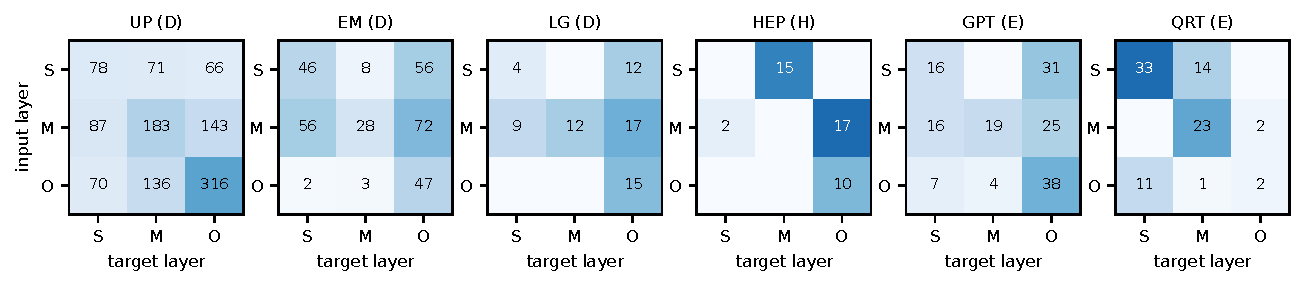
\includegraphics[width=\textwidth]{fig_signatures.pdf}
\caption{Layer-pair signatures of the six branches (rows: input layer; columns: target layer; shading normalised per branch). For HEP the record-level matrix of the final step is shown (a generic layer edge counted once, an AND route once, plus the ten observable-family edges), so that the expansion of generic edges does not inflate the S$\to$M entry.}\label{fig:signatures}
\end{figure}
\begin{table}[htbp]\centering\small
\caption{Layer-pair signatures $\Sigma(G)$ (leg--route incidences). The last row gives the record-level signature of the HEP final step.}\label{tab:signatures}
\begin{tabular}{@{}lrrrrrrrrr@{}}\toprule
 & \multicolumn{3}{c}{S $\to$} & \multicolumn{3}{c}{M $\to$} & \multicolumn{3}{c}{O $\to$} \\
 & S & M & O & S & M & O & S & M & O \\\midrule
UP & 78 & 71 & 66 & 87 & 183 & 143 & 70 & 136 & 316 \\
EM & 46 & 8 & 56 & 56 & 28 & 72 & 2 & 3 & 47 \\
LG & 4 & 0 & 12 & 9 & 12 & 17 & 0 & 0 & 15 \\
HEP & 0 & 68 & 0 & 20 & 14 & 17 & 0 & 0 & 10 \\
GPT & 16 & 0 & 31 & 16 & 19 & 25 & 7 & 4 & 38 \\
QRT & 33 & 14 & 0 & 0 & 23 & 2 & 11 & 1 & 2 \\
HEP (records) & 0 & 15 & 0 & 2 & 0 & 17 & 0 & 0 & 10 \\
\bottomrule\end{tabular}

\end{table}
\Cref{fig:signatures} and \cref{tab:signatures} give the signatures. Three patterns are visible and they define the branch types.

\begin{definition}[Branch types]\label{def:types}
\begin{itemize}[nosep]
\item \textbf{Type D (dynamic / pedagogical).} Routes have AND logic and combine model and state nodes (and observables) into states and observables; the support of $\Sigma$ contains $(\lay M,\lay S)$, $(\lay M,\lay O)$, $(\lay S,\lay O)$ and usually $(\lay O,\lay O)$. Observables may be primitive (no route into them). The time axis is a reading order and the graph is a filtration.
\item \textbf{Type H (historical theory-building).} The support of $\Sigma$ is contained in the set $\{(\lay S,\lay M),\allowbreak(\lay M,\lay O),\allowbreak(\lay M,\lay S),\allowbreak(\lay M,\lay M),\allowbreak(\lay O,\lay O)\}$: state sectors enter model nodes by AND routes whose legs are (sector, occupation number) pairs, model nodes reach observables, model nodes act back on the state layer, model nodes have lineage, and observables refine one another. The model layer is the moving part; nodes are removed and merged.
\item \textbf{Type E (effect / resource).} All routes are single edges; the observable layer is split into witnesses, effects and tasks with a witness--effect pairing; the state layer is refined into clusters or free/resource sets; the model layer is fixed (quantum theory and its neighbours) or a lattice of theories; the support contains $(\lay S,\lay O)$ directly.
\end{itemize}
\end{definition}

\section{The layer discipline of the historical graph}
\begin{proposition}[Layer discipline, verified on the data]\label{prop:discipline}
In every one of the \NhepStepsGraph{} step graphs of the Standard Model branch (\NhepRoutesChecked{} expanded routes in all): (i) no route has a state target and a state input; (ii) no route has an observable input; (iii) every route of kind \id{predicts}, \id{calibrates}, \id{frames} or \id{candidate} with a single input leaves a model node; (iv) every AND route has only state legs and a model target. Consequently every directed path from a state node to an observable node passes through a model node.
\end{proposition}
\begin{proof}
(i)--(iv) are checked exhaustively by the engine (\texttt{replay\_hep.py}, field \texttt{invariants}): the violation counts are \NhepInvStoSroutes{}, \NhepInvOasinput{}, \NhepInvmTwoofromnonM{} and \NhepInvandrouteswithnonSleg{}+\NhepInvandroutesintononM{}. For the consequence: a path from $s\in\VS$ to $o\in\VO$ consists of routes; the route that enters $o$ has, by (ii) and (iii) and because AND routes have model targets by (iv), a model-node input; hence the path contains a model node.
\end{proof}
The proposition is the formal content of the convention stated when the branch was built (``edges to observables only from model-layer nodes; edges into model nodes only from state sectors''). It is also the structural difference between type H and type E: in the nonclassicality network \NGPTPairStoO{} leg--route incidences go from the state layer straight into the observable layer, in the resource-theory network \NQRTPairOtoS{} go from witnesses into states.

\section{Effect networks as fibres: the contraction lemma}\label{sec:contraction}
\begin{proposition}[Contraction and lift]\label{prop:contraction}
Let $G$ be a concept graph and $m_0\in\VM$ a model node. Define the \emph{contraction} $G/m_0$ by deleting $m_0$ and its routes and adding, for every pair of single routes $(s\to m_0,\ m_0\to o)$ with $s\in\VS$ and $o\in\VO$, the route $s\to o$ with the kind and status of $m_0\to o$ and the label $m_0$. Then
\begin{enumerate}[nosep]
\item $\Sigma(G/m_0)_{\lay S\lay O}=\Sigma(G)_{\lay S\lay O}+\indeg_{\lay S}(m_0)\cdot\outdeg_{\lay O}(m_0)$, where the degrees count single routes into $m_0$ from state nodes and out of $m_0$ into observables;
\item the \emph{lift} $(G/m_0)\!\uparrow\! m_0$, which re-inserts $m_0$ and replaces every route labelled $m_0$ by the two routes through $m_0$, recovers $G$ whenever $m_0$'s other routes (back-edges, lineage) are stored with the label;
\item if every state node of $G$ has a route into $m_0$ (a fixed model), then $G/m_0$ has no model node adjacent to those states, i.e.\ it is of type E with respect to $m_0$.
\end{enumerate}
\end{proposition}
\begin{proof}
(1) Each deleted pair contributes one new $\lay S\to\lay O$ incidence and the pairs are in bijection with $I\times O$ for $I$ the set of state in-neighbours and $O$ the set of observable out-neighbours of $m_0$. (2) The label identifies the pairs; re-inserting $m_0$ and splitting each labelled route into $s\to m_0$ and $m_0\to o$ restores the deleted routes, and the stored remaining routes restore the rest. (3) After contraction no route between a state node and $m_0$ exists, and the state--observable routes carry $m_0$ only as a label.
\end{proof}
\begin{corollary}
The direct state--effect edges of the quantum networks (\NGPTPairStoO{} in GPT, 21 of which have an effect node as target) are the contracted form of two-step paths through the hosting model. In the lifted graph every such edge becomes $s\to m\to e$ with $m$ the model node that hosts $s$ (quantum theory for the quantum state clusters; the network records the hosting relation explicitly by its \id{hosts} edges for entangled states in four models).
\end{corollary}
The corollary answers the question why the quantum networks can draw states into observables directly: they are drawn \emph{inside one model}. When the model layer varies, as in the readers and in the history, the model must be written on the path. This is not a difference of philosophy between the instances but a difference of what is held fixed, and \cref{prop:contraction} is the dictionary between the two drawings.

\section{Effects as clusters of observables}\label{sec:families}
In the quantum networks an \emph{effect} is a phenomenon (Bell violation, steering, contextuality) and a \emph{witness} is the operator-valued test that detects it; the network pairs them one-to-one (\id{pairs} edges) with the recorded exception of a stratified functional. An effect is therefore the class of all direct observables whose outcome statistics the witness evaluates: a Bell functional is one number computed from many correlators. In the normalised schema an effect is an observable node of sub-layer \emph{effect} together with its witness, and the direct observables behind it are not drawn because the branch treats them as the witness's input data. The same coarse-graining is present in the historical graph, where it is drawn: the Standard Model data types its observables as $\sigma$-type (cross sections: Compton, pair production, neutral-current events, triple-gauge couplings, Higgs rates), $\Gamma$-type (widths and lifetimes: $\beta$ decay, neutron and muon lifetimes) and parameters, with the generic nodes $\sigma$, $\Gamma$ and ``particle production and decay'' as family heads; the step that introduces the field node rewrites the generic observable into the two families, and the specific processes refine them. The engine records these as ten \id{subset} routes among observables (\cref{fig:signatures}, HEP entry $\lay O\to\lay O$), and uses them in \cref{ch:hep}: a family head counts as explained when one member is.

Thus the three types use three resolutions of the observable layer: primitive measurements (D), families of measurements with a head (H), and effects with a witness (E). The grand network keeps all three as sub-layers; the family and the witness--effect pair are both instances of one operation, \op{cluster} applied to the observable layer.

\section{Roles are branch-relative: the gluing and the role flips}\label{sec:flips}
The branches share concepts. The engine glues them through a curated table of \NnConcepts{} concepts (\cref{app:concepts}), each listing its member nodes per branch with a one-line justification taken from the node labels and descriptions; a node belongs to at most one concept and \NnGlued{} nodes are glued. \NnCross{} looser relations (part-of, refinement, model-of) are kept separately as cross-edges and are not identifications. Of the \NnConcepts{} concepts, \NnConceptsReaders{} join only the three readers, \NnConceptsQuantumInfo{} join only the two quantum networks, and \NnConceptsBridge{} bridge the groups; \NnConceptsThreePlus{} concepts are shared by three or more branches (position; Faraday's law; the electromagnetic field state; Planck's constant; the photon; the Schr\"odinger equation, in four branches; the Hilbert-space state; the Gibbs state; the second law).

\begin{table}[htbp]\centering\small
\caption{The \NnFlips{} role flips: concepts whose layer differs between branches.}\label{tab:flips}
\begin{longtable}{@{}p{3.2cm}p{3.0cm}p{8.4cm}@{}}\toprule
Concept & Role per branch & Why the role differs \\\midrule\endhead
Planck's constant & EM: O, UP: O, GPT: M & a measured constant (observable) in both readers; an axiom (deformation scale) in the nonclassicality network. \\
Blackbody radiation / spectrum & EM: O, UP: S & EM records the measured spectrum (observable); UP records the equilibrium radiation I(lambda, T) as a state. \\
Photon & EM: O, UP: S, HEP: S & EM detects the photon one at a time (observable); UP treats the photon (E = hf, p = hbar k) as a state; HEP has the photon Fock sector (state). \\
Bohr model / orbits & EM: S, UP: M & EM records Bohr orbits as a hybrid state; UP records Bohr's postulates as a model. \\
Hydrogen energy levels & UP: S, HEP: O & UP lists the allowed levels as states; HEP records the spectrum of H as an observable (E\_n = -m e\^{}4 / 2 hbar\^{}2 n\^{}2). \\
Particle production and decay & UP: S, HEP: O & UP lists the nuclear decay channels as a state (what a nucleus becomes); HEP records production/decay as the observable that forces the Fock extension. \\
Second law(s) of thermodynamics & UP: M, GPT: O, QRT: O & a model-layer law in the textbook; in the quantum branches the second laws are observable-layer tests (a task in GPT; the F\_alpha monotone family in QRT) on state conversion. \\
Two-path (second-order) interference & UP: S, GPT: O & UP records the double-slit pattern as a wave state; GPT records second-order interference as an effect detected by fringe visibility. \\
Bell nonlocality & GPT: O, QRT: S & an effect (violation) in GPT; the resource (nonlocal boxes) in QRT. \\
EPR steering & GPT: O, QRT: S & an effect in GPT; the resource (steerable assemblages) in QRT. \\
Kochen-Specker contextuality & GPT: O, QRT: S & effects (state-independent and state-dependent KS) in GPT; the resource (contextual behaviors) in QRT. \\
Measurement incompatibility & GPT: O, QRT: S & an effect in GPT; a device resource (incompatible POVM sets) in the state layer of QRT. \\
Device-independent tasks & GPT: O, QRT: M & a task (observable layer) in GPT; the resource-utilizing operation class (model layer) in QRT. \\
One-sided device-independent tasks & GPT: O, QRT: M & ROLE FLIP as for di\_tasks. \\
State injection / universal computation & GPT: O, QRT: M & ROLE FLIP as for di\_tasks. \\
Parity-oblivious multiplexing / RAC advantage & GPT: O, QRT: M & ROLE FLIP as for di\_tasks. \\
Metrology / clocks & GPT: O, QRT: M & postselected metrology as a task in GPT; metrology and clocks as asymmetry-utilizing operations in QRT. \\
\bottomrule\end{longtable}

\end{table}
\Cref{tab:flips} lists the \NnFlips{} concepts whose layer differs between branches. They are not errors of one branch or the other. The photon is \emph{detected} in the history of electromagnetism (an observable: one photon at a time in a photomultiplier), \emph{posited} in the textbook (a state with $E=hf$) and \emph{a sector} in the Standard Model graph (the Fock sector that the field creates). Planck's constant is a measured number in the readers and the deformation scale of the Moyal lift in the nonclassicality network, where it is an axiom. The second law is a model-layer law in the textbook and, in the quantum networks, a family of observable-layer tests on state conversion. Bell nonlocality, steering, Kochen--Specker contextuality and incompatibility are effects in the nonclassicality network and resource states in the resource-theory network; the device-independent and metrological tasks are observable-layer tasks in one and resource-utilising operation classes (model layer) in the other. The conclusion is that \emph{role is a function of the branch's epistemic process}, not of the concept: the layer of a concept records what the branch does with it (measure it, posit it as what exists, hypothesise it as a law or an operation). The grand network therefore stores the triple (concept, branch, role), and the flips are the places where two branches use one concept for two purposes. Several cross-edges carry further flips of the same kind: the S-matrix is a state-layer node in the electromagnetism reader and the rewritten observable postulate (model layer) in the history; the radioactive decay law, a model-layer law in the textbook, refines the decay width, an observable in the history; the positron, an observable in the electromagnetism reader, lives in the electron sector of the history.

\section{The atlas}\label{ch:atlas}
\begin{figure}[htbp]\centering
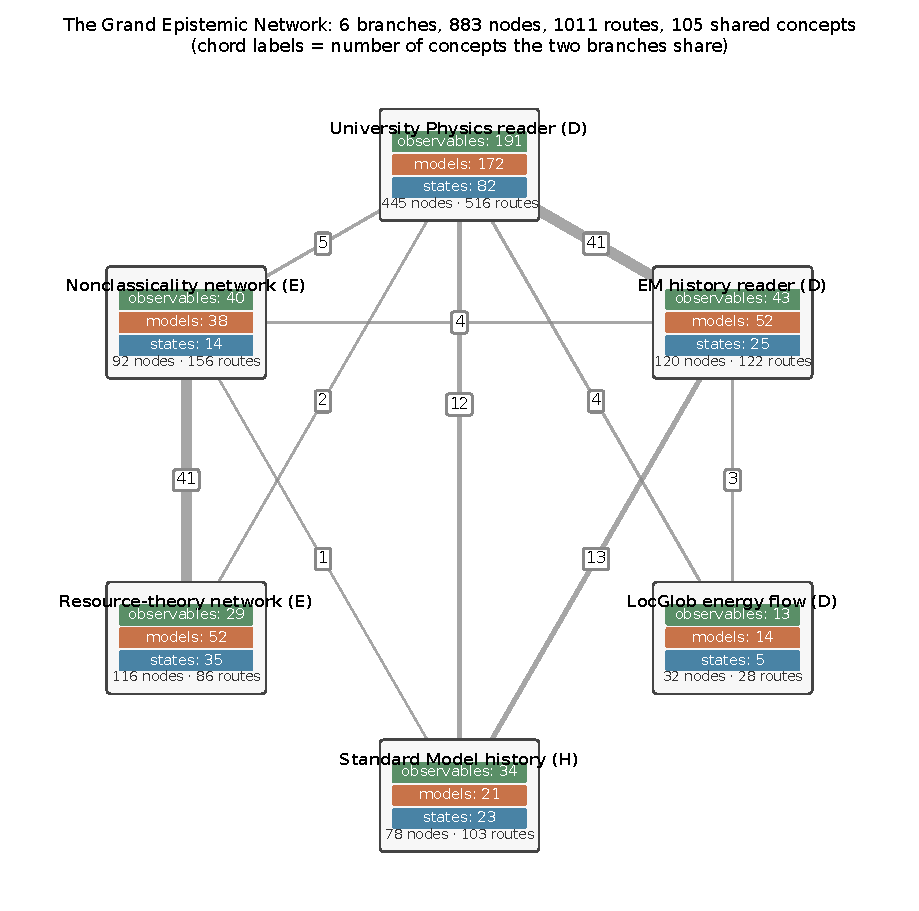
\includegraphics[width=0.9\textwidth]{fig_atlas.pdf}
\caption{The grand network as an atlas: six branch graphs with their layer sizes, joined by chords whose labels count the concepts the two branches share.}\label{fig:atlas}
\end{figure}
\Cref{fig:atlas} draws the merged network as an atlas. \NnConceptsReaders{} concepts involve only the three readers (the electromagnetism history and the textbook share 41 concepts in all, a few of them also present in another branch); \NnConceptsQuantumInfo{} involve only the two quantum networks; the \NnConceptsBridge{} bridges are the classical-to-quantum concepts of the electromagnetism reader (Poisson bracket and canonical commutator, glued to the genesis axioms of the nonclassicality network; Planck's constant; the Schr\"odinger equation, glued to unitary evolution in the history and to the unitary process cluster of the nonclassicality network; the Hilbert-space state, which the quantum state clusters refine), the quantum-electrodynamics concepts shared by the electromagnetism reader and the history (the QED vertex, the Lamb shift, the anomalous moment, the fine-structure constant, cross sections, creation and annihilation operators, the electron field), the textbook--history concepts (Compton effect, spin, angular momentum, hydrogen levels, decays, the Standard Model), and the thermodynamic concepts (Gibbs state, second law) shared by the textbook and the quantum networks. The data file \texttt{gen\_grand\_network.json} (\cref{app:data}) holds all nodes and routes with their universal and native fields, the concepts with roles, the cross-edges and the cluster records of the Standard Model.

%=====================================================================
\chapter{Operations and rules}\label{ch:rules}

\section{Primitive operations}
Every change of a concept graph in the six instances decomposes into the operations of \cref{tab:ops}. The table states the layer on which each operation acts, its effect on the node count of that layer and on the route count in the elementary case, and the rule that fires it. The operations of the Standard Model page's operation log (\op{add}, \op{rewrite}, \op{partition}, \op{extend}, \op{split}, \op{replace}, \op{merge}, \op{absorb}, \op{cluster}, \op{lineage}, \op{route}, \op{predict}, \op{calibrate}, \op{flag}, \op{signal}, \op{back}) are taken as they are; the readers add \op{derive} and \op{fail}; the inference engine of the project adds \op{compose} and \op{reduce}; \cref{sec:contraction} adds \op{contract} and \op{lift}; the quantum networks add \op{census} and \op{close}.
\begin{table}[htbp]\centering\scriptsize
\caption{Primitive operations with their count deltas.}\label{tab:ops}
\begin{longtable}{@{}p{1.7cm}p{2.2cm}p{2.3cm}p{3.0cm}p{5.4cm}@{}}\toprule
Operation & layer & $\Delta$ nodes & $\Delta$ routes & meaning \\\midrule\endhead
\texttt{ADD} & S|M|O & +1 & +k (k = routes attached on arrival) & a new node appears \\
\texttt{REWRITE} & S|M|O & 0 & 0 or re-attached & a node keeps its identity and changes its content \\
\texttt{PARTITION} & S & +(k-1) & +k back-edges & a state node is replaced by the k irreducible components of a symmetry representation (R1) \\
\texttt{EXTEND} & S & 0 (ladders are internal) & +1 back-edge per sector & each irreducible block becomes a Fock ladder (R3) \\
\texttt{SPLIT} & S & +1 & routes re-attached & a sector splits in two after an observable distinguishes them (R8) \\
\texttt{REPLACE} & S & 0 & routes re-attached & k sectors are replaced by k others after an observable shows compositeness (R8) \\
\texttt{MERGE} & M & -(k-1) & routes = union & k model nodes that share a calibration become one (R6) \\
\texttt{ABSORB} & M & -1 eff, +1 fund, +sectors & +1 leg per route; +lineage & an effective node becomes the low-energy limit of a fundamental one (R7) \\
\texttt{CLUSTER} & M & +1 cluster per term & routes re-attached to clusters; +member/lineage edges & fundamental nodes grouped by Lagrangian term (R10) \\
\texttt{LINEAGE} & M->M & 0 & +1 & an absorption trace recorded inside a cluster \\
\texttt{ROUTE} & S->M & 0 & +1 AND route & legs = (sector, n) pairs of the fields of a term (R4) \\
\texttt{PREDICT} & M->O & 0 & +1 & a model node reaches an observable (status pred) \\
\texttt{CALIBRATE} & M->O & 0 & +1 (status fit) & an observable fixes a parameter (R9) \\
\texttt{FLAG} & O & 0 & 0 & an observable has in-degree 0 from the model layer (R2 precondition) \\
\texttt{SIGNAL} & M & 0 & 0 & two model nodes share a calibration edge (R6 precondition) \\
\texttt{BACK} & M->S & 0 & +1 & a model node acts on the state layer \\
\texttt{DERIVE} & M∧S->S|O (type D) & 0 or +1 & +1 AND route & a reading-indexed route combines model and state nodes (readers) \\
\texttt{FAIL} & route & 0 & 0 (route marked failed) & a prediction route fails; a later route to the same target resolves it \\
\texttt{COMPOSE} & S & +1 (tensor sector) & +routes & a new independent sector is adjoined by tensor product (Rule II of the inference engine) \\
\texttt{REDUCE} & M|S & -(k-1) & 0 & parameters tied by symmetry, representation reduced by the commutant (Rule III of the inference engine) \\
\texttt{CONTRACT} & M & -1 & S->O direct edges replace 2-paths & a fixed model node is suppressed: an H-graph becomes an E-graph (Prop. contraction) \\
\texttt{LIFT} & M & +1 & 2-paths replace S->O edges & inverse of CONTRACT \\
\texttt{CENSUS} & layer pair & 0 & 0 & enumerate the cells (pairs) of a layer pair with no recorded edge \\
\texttt{CLOSE} & edge & 0 & +1 & settle a cell by composition, elementary proof, counterexample or literature fill \\
\bottomrule\end{longtable}

\end{table}

\begin{proposition}[Count deltas, verified on the history]\label{prop:deltas}
On the Standard Model data the deltas of \cref{tab:ops} are realised as follows: \op{partition} at Step 2 takes the state count from 1 to 9 ($+8$ for $k=9$ classes); \op{extend} at Step 4 takes it from 9 to 5 with no new irreducible block (the classes without a realised particle and the vacuum are not separate sectors, and three species share the $m>0$, $s=\tfrac12$ class); \op{split} at Step 7 adds one state node net of the split ($\nu\to\nu_e,\nu_\mu$) and \op{add} one more ($\mu$); \op{merge} at Step 8 takes the model count from 6 to 5; \op{absorb} at Step 9 removes one effective node, adds three fundamental nodes and two mediator sectors; \op{cluster} at Step 12 replaces eight model nodes by six clusters. The trajectories are $S$: \NhepTrajS; $M$: \NhepTrajM; effective: \NhepTrajEff; fundamental: \NhepTrajFund; AND routes: \NhepTrajAND.
\end{proposition}
\begin{proof}
Read off \cref{tab:steps}, which is computed from the data by the replay of \cref{ch:hep}.
\end{proof}

\section{Rules as guarded operations}
A \emph{rule} is a pair (predicate on $G_t$, operation schema): when the predicate holds, the operation is enabled. The ten rules of the Standard Model paper are restated here in that form, with the predicate written so that the engine can evaluate it. Notation: $N^-_{\lay M}(o)$ is the set of model nodes with a single route of kind \id{predicts}, \id{calibrates} or \id{frames} into $o$ (framework assignments flagged weak and candidate edges excluded); $\dim[g]$ is the mass dimension of the coupling of an interaction node, recorded in the data as the node kind \emph{eff} ($\dim[g]<0$) or \emph{fund} ($\dim[g]=0$); a route $(L,m)$ has legs $L\subseteq\VS\times\mathbb N$ and head $m\in\VM$.

\begin{rule_}[R1, symmetry partition]
Predicate: a framework node $m$ represents a symmetry group on a state node $s$ (in the data: a back-edge $m\to s$ from a rewritten framework node; Wigner's classification of the Poincar\'e group \citep{wigner1939} is the instance). Operation: \op{partition} $s$ into the irreducible components $\{s_i\}$, each receiving the back-edge; the labels of the components (Casimir invariants) become observables with routes $m\to o$ of status \emph{pred} (badge P).
\end{rule_}
\begin{rule_}[R2, in-degree-zero drive]
Predicate: $\exists o\in\VO$ with $N^-_{\lay M}(o)=\emptyset$ (an \emph{unexplained} observable), or the model layer is inconsistent on theory-internal grounds (recorded in the data by the step driver). Operation: \op{add} a model node $m$ with a route $m\to o$; in the theory-internal case $m$ must reproduce every route of the node it replaces. No model node is added otherwise. A candidate node (kind \emph{cand}) announces the rule without executing it.
\end{rule_}
\begin{rule_}[R3, Fock extension]
Predicate: the repairing node of R2 connects states of different particle number. Operation: \op{extend} \citep{fock1932,weinberg1995}: every irreducible block $\mathcal H_s$ becomes the ladder $\bigoplus_N \mathrm{Sym}^N\mathcal H_s$ or $\bigoplus_N\Lambda^N\mathcal H_s$ by the back-edge of the new node; no new irreducible block is introduced.
\end{rule_}
\begin{rule_}[R4, route composition]
Predicate: an interaction node $m$ with a Lagrangian term. Operation: \op{route}: one AND route into $m$ per sector combination the term couples, with legs the (sector, minimal occupation change) pairs of the fields in the term.
\end{rule_}
\begin{rule_}[R5, effective status]
Predicate: a model node with $\dim[g]<0$. Operation: mark it effective (dashed): its observable routes are valid for $q^2\ll\Lambda^2$ and it cannot be final.
\end{rule_}
\begin{rule_}[R6, universality merge]
Predicate: two coexisting model nodes share a calibration edge into the same observable (in the data this appears either as two \id{calibrates} routes into one observable or as the transfer of the calibration edge from one node to a second while the first persists). Operation: \op{merge} them into one node whose routes are the union of theirs (the universal V$-$A interaction \citep{feynman_gellmann1958,sudarshan_marshak1958} merging Fermi's term \citep{fermi1934} with the muon-decay term).
\end{rule_}
\begin{rule_}[R7, absorption]
Predicate: an effective node $m_{\rm eff}$ and a fundamental node $m_{\rm fund}$ with a new mediator sector $s$ such that every route of $m_{\rm eff}$ is covered by routes of $m_{\rm fund}$ once the leg $s(1)$ is removed. Operation: \op{absorb}: remove $m_{\rm eff}$, record the lineage $m_{\rm eff}\to m_{\rm fund}$, and add the further fundamental nodes that the symmetry forces, with their predicted observables (badge P); the electroweak gauge theory \citep{glashow1961,weinberg1967} absorbing V$-$A is the instance.
\end{rule_}
\begin{rule_}[R8, sector refinement]
Predicate: a state node changes. Operation: only \op{partition} (R1), \op{extend} (R3), \op{split} (an observable distinguishes two instances of the same irreducible block, as the two-neutrino experiment did \citep{danby1962}) or \op{replace} (an observable shows compositeness; $k$ sectors replaced by $k$ with the same blocks). The state layer never changes from a state node.
\end{rule_}
\begin{rule_}[R9, calibration]
Predicate: a model node with $p$ free parameters. Operation: \op{calibrate}: $p$ routes of status \emph{fit} (badge F); the predictive content of the node is its number of observable routes minus $p$.
\end{rule_}
\begin{rule_}[R10, clustering]
Predicate: no effective node outside a fundamental one. Operation: \op{cluster} the fundamental nodes by Lagrangian term; absorbed nodes sit inside the cluster whose member reproduces them; routes and observable edges are re-attached to the clusters.
\end{rule_}
The readers add two rules.
\begin{rule_}[R11, reading-order growth]
Predicate: the next paragraph of the text. Operation: \op{add} the node at the paragraph that introduces it and \op{derive} the route at the paragraph that explains it; no route precedes its inputs or its target.
\end{rule_}
\begin{rule_}[R12, failed-route resolution]
Predicate: a route marked \emph{failed} into $o$. Operation: a later non-failed route into $o$ (of another kind family) resolves it; the distance in paragraphs is recorded.
\end{rule_}
The quantum networks add two rules, which are the operational form of the project's aim to generate research ideas automatically. Their edges are theorems of the generalised-probabilistic-theory and resource-theory literature \citep{spekkens2005,plavala2016,barnum2007,schmid2021,aubrun2022,howard2014,marvian2016,chitambar2019,takagi2019,lostaglio2018}; the rules say how the edge set grows.
\begin{rule_}[R13, census]
Predicate: a designated layer pair $(a,b)$ (witness $\times$ state $\times$ process; theory $\times$ theory; node pairs). Operation: \op{census}: enumerate the pairs with no recorded edge; each is a candidate theorem.
\end{rule_}
\begin{rule_}[R14, closure]
Predicate: an uncharted cell. Operation: \op{close} it by one of four routes: composition of existing edges, elementary proof, counterexample, or literature fill; the new edge carries the route as its status (derived, counterexample, theorem) and no edge means \emph{unsettled}, never false.
\end{rule_}
The inference engine of the project (\cref{sec:solvers}) adds the two rules that act on a model's \emph{sectors}: \op{compose} (adjoin an independent sector by tensor product when the refit of the old structure cannot explain new data) and \op{reduce} (tie parameters when the evidence favours the symmetry and decompose the representation by the commutant of the model's own operator algebra). They are listed as R15 and R16 and are not exercised on the six graphs, which record their outputs (sectors, merged nodes) rather than their runs.

\section{The agenda theorem}
\begin{definition}[Agenda]
For a concept graph $G$ with designated census pairs $\mathcal C$, the \emph{agenda} is
\[A(G)=U(G)\ \cup\ C(G)\ \cup\ Q(G)\ \cup\ E(G)\ \cup\ F(G)\ \cup\ P(G),\]
where $U(G)=\{o\in\VO: N^-_{\lay M}(o)=\emptyset\}$ (unexplained observables), $C(G)$ is the set of uncharted cells of $\mathcal C$, $Q(G)$ the set of pairs of model nodes sharing a calibration edge, $E(G)$ the set of effective nodes, $F(G)$ the set of failed routes without a forward resolver, and $P(G)$ the set of untested predictions (observable nodes flagged untested or candidate edges).
\end{definition}
\begin{theorem}[Agenda]\label{thm:agenda}
$A(G)$ is computable in time $O\big(|V|+\sum_{r\in R}|I_r|+|\mathcal C|\big)$.
\end{theorem}
\begin{proof}
$U(G)$: one pass over the routes marks every observable with an incoming single route from a model node of the three explanatory kinds; the unmarked observables are $U(G)$. $Q(G)$: one pass over the calibration routes groups model nodes by target; pairs within a group are $Q(G)$ (their number is bounded by the number of calibration routes squared, which in the data never exceeds two per observable). $E(G)$ and $P(G)$: one pass over the nodes. $F(G)$: for each failed route, the forward resolver is the minimum-time non-failed route into the same target, found in one pass per target after sorting the routes once by time, $O(|R|\log|R|)$ in the worst case and linear when the routes are stored in time order as the readers store them. $C(G)$: one pass over the designated cells with a lookup of recorded verdicts.
\end{proof}
The theorem is modest, and that is its point: the \emph{location} of the next question is computed, not judged. For the six graphs the agenda is listed in \cref{ch:explore}; the quantum networks and the Standard Model page already compute parts of it (the red ring of an unexplained observable, the grey cells of the witness matrix), and the engine computes all parts for all branches with one code path.

\begin{proposition}[Monotone closure]\label{prop:closure}
Under \op{close} alone the number of uncharted cells $|C(G)|$ strictly decreases and the process terminates after at most $|\mathcal C|$ steps. Under \op{add} of a node of layer $a$ the number of cells increases by $\sum_{b}|V_b|$ over the partner layers $b$ of $a$ in $\mathcal C$, so the census of a growing graph is bounded by the product of the layer sizes.
\end{proposition}
\begin{proof}
Immediate from the definitions; a closed cell is never reopened (its edge keeps its status), and the cells of a new node are its pairs with the existing partner layer.
\end{proof}

\section{The loop}
\begin{figure}[htbp]\centering
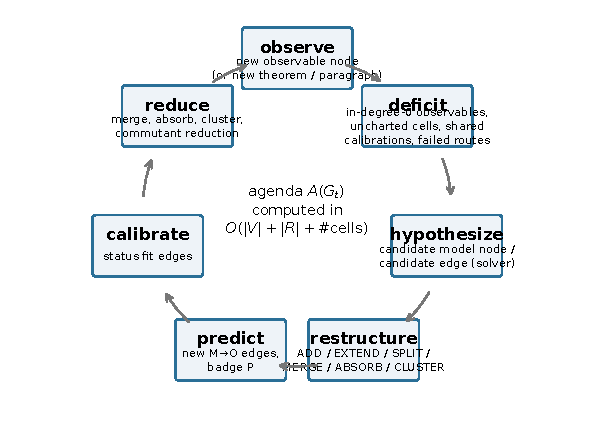
\includegraphics[width=0.7\textwidth]{fig_cycle.pdf}
\caption{The loop the instances run. Every box except \emph{hypothesize} is executed by the engine on the graph; \emph{hypothesize} calls a solver. The agenda at the centre is recomputed after each step (\cref{thm:agenda}).}\label{fig:cycle}
\end{figure}
Rules R2--R7 compose into a loop (\cref{fig:cycle}): an unexplained observable appears (R2), a model node repairs it and, if needed, extends the state layer (R3), its routes are read off its term (R4), a dimensionful coupling marks it temporary (R5), nodes sharing a coupling merge (R6), the merged node is absorbed by a fundamental one with a new sector and the symmetry predicts further observables (R7), the fundamental nodes cluster (R10). The quantum networks run the same loop with \op{census} in the place of the red ring and \op{close} in the place of the model node. The readers run it in replay: every failed route is the \emph{deficit} phase, every resolving route the \emph{restructure} phase of a loop that the text narrates.

%=====================================================================
\chapter{Regenerating the historical graph: the Standard Model replay}\label{ch:hep}

\section{The data and the two views}
The released file of the Standard Model branch records twelve graph steps (a thirteenth, the synthesis, has no graph of its own). For each step it lists the state, model and observable nodes drawn and the edges and AND routes among them, together with the method phases active at the step and a hand-written operation log. The page draws a \emph{selection} of observables at every step for readability: the spectra of one-particle quantum mechanics (position, momentum, angular momentum, spin, the energy levels) are dropped between Steps 2 and 4, the generic width and cross section after Step 4, and so on; \NhepOCumFinal{} distinct observables exist over the sequence while the final step draws \NhepOShownFinal{}. The engine therefore keeps two views: the \emph{page view}, the graph exactly as drawn at each step, on which the rule predicates are evaluated and which is the object the hand-made tables describe; and the \emph{cumulative view}, in which an observable, once measured, stays in the graph, and a model$\to$observable route persists through the successors of its source node (the successor of a removed model node is derived from the data: the single node added when it is removed, for Steps 4 and 8; the lineage edges of the final clusters, for Step 9; cluster membership, for Step 12). The cumulative view is the state of knowledge; the page view is its drawing.

\begin{table}[htbp]\centering\scriptsize
\caption{Per-step counts of the Standard Model graph, page view and cumulative view. ``edge records'' counts the edge records of the data file (a generic layer edge once); ``F edges'' are calibration edges; ``deficit'' is the number of unexplained observables.}\label{tab:steps}
{\setlength{\tabcolsep}{3.5pt}\begin{tabular}{@{}rlrrrrrrrrrrrr@{}}\toprule
Step & id & S & M & O$_{\rm shown}$ & O$_{\rm cum}$ & records & AND & eff & fund & cl. & F & def.$_{\rm shown}$ & def.$_{\rm cum}$ \\\midrule
1 & qm & 1 & 3 & 5 & 5 & 9 & 0 & 0 & 0 & 0 & 0 & 0 & 0 \\
2 & wigner & 9 & 3 & 6 & 7 & 10 & 0 & 0 & 0 & 0 & 0 & 0 & 0 \\
3 & anomaly & 9 & 3 & 6 & 8 & 9 & 0 & 0 & 0 & 0 & 0 & 1 & 1 \\
4 & fock & 5 & 3 & 4 & 10 & 9 & 0 & 0 & 0 & 0 & 0 & 2 & 3 \\
5 & qed & 5 & 4 & 6 & 16 & 10 & 1 & 0 & 1 & 0 & 1 & 1 & 2 \\
6 & fermi & 5 & 5 & 6 & 18 & 11 & 2 & 1 & 1 & 0 & 2 & 0 & 0 \\
7 & muon & 7 & 6 & 9 & 21 & 14 & 3 & 2 & 1 & 0 & 2 & 0 & 0 \\
8 & va & 7 & 5 & 11 & 23 & 16 & 4 & 1 & 1 & 0 & 2 & 0 & 0 \\
9 & ew & 9 & 7 & 12 & 29 & 17 & 7 & 0 & 4 & 0 & 3 & 0 & 0 \\
10 & higgs & 10 & 10 & 13 & 33 & 19 & 8 & 0 & 7 & 0 & 4 & 0 & 0 \\
11 & frontier & 10 & 11 & 12 & 34 & 18 & 9 & 0 & 7 & 0 & 3 & 1 & 1 \\
12 & sm & 10 & 9 & 16 & 34 & 22 & 12 & 0 & 0 & 6 & 4 & 1 & 1 \\
\bottomrule\end{tabular}}

\end{table}

\begin{figure}[htbp]\centering
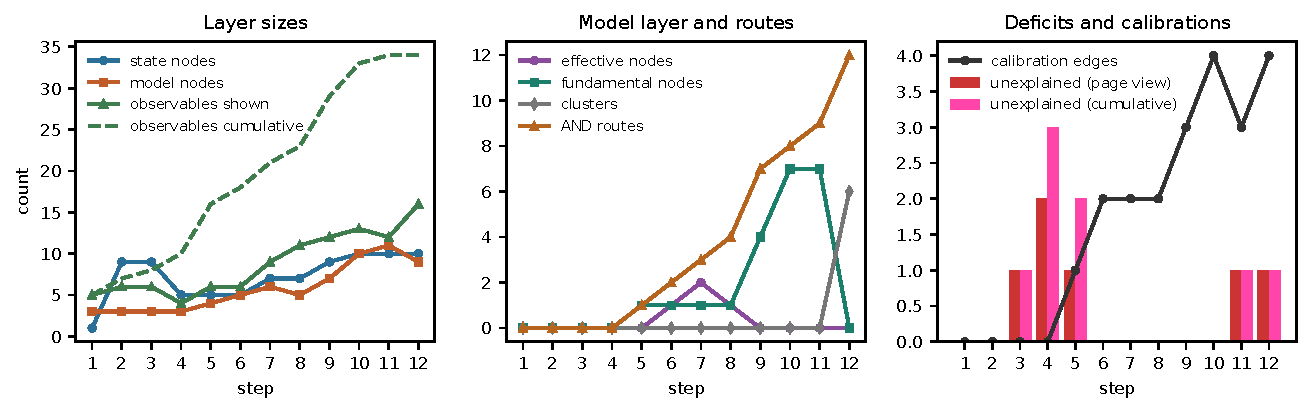
\includegraphics[width=\textwidth]{fig_hep_trajectories.pdf}
\caption{Trajectories across the twelve steps: layer sizes (left; dashed: cumulative observables), model-layer composition and AND routes (middle), deficits and calibration edges (right).}\label{fig:hep}
\end{figure}

\section{Decomposition into operations}
For each pair of consecutive steps the engine computes the set differences of nodes and routes and decomposes them into the operations of \cref{tab:ops} by structural tests only (layers, node kinds, the irreducible-representation label of a sector, the A/P/F badge of an observable, route kinds and AND-route leg sets; no step text is read). \Cref{tab:oplog} is the resulting log. It should be read against the hand-written operation log on the page; the two agree in content, and the engine's version is reproducible.
\begin{table}[htbp]\centering\scriptsize
\caption{Decomposition of every step transition into primitive operations, computed from the data.}\label{tab:oplog}
\begin{longtable}{@{}p{0.6cm}p{1.9cm}p{1.3cm}p{10.5cm}@{}}\toprule
Step & Operation & Layer & Decomposition read off the data \\\midrule\endhead
2 & \texttt{PARTITION} & S & H1 -> 9 irreducible classes (back-edge of a rewritten model node) \\
\addlinespace[2pt]
3 & \texttt{FLAG} & O & new unexplained observable o\_prod: precondition of R2 \\
\addlinespace[2pt]
4 & \texttt{EXTEND} & S & 9 classes -> 5 sectors with ladders, by the back-edge of m\_field \\
 & \texttt{ADD} & M & m\_field; deficit o\_prod rewritten into finer observables \\
\addlinespace[2pt]
5 & \texttt{ADD} & M & m\_qed; deficit o\_sig, o\_G rewritten into finer observables; explains the observed-before-explained o\_compton, o\_ae, o\_lamb \\
 & \texttt{ROUTE} & S->M & 1 new AND route(s): m\_qed <- 2 leg(s) \\
 & \texttt{CALIBRATE} & O->M & calibration edge(s) added for o\_alpha; new parameter(s): o\_alpha \\
\addlinespace[2pt]
6 & \texttt{ADD} & M & m\_fermi; reaches the open deficit o\_beta \\
 & \texttt{ADD} & M(eff) & effective node(s) m\_fermi: dimensionful coupling, temporary by construction \\
 & \texttt{ROUTE} & S->M & 1 new AND route(s): m\_fermi <- 4 leg(s) \\
 & \texttt{CALIBRATE} & O->M & calibration edge(s) added for o\_GF; new parameter(s): o\_GF \\
\addlinespace[2pt]
7 & \texttt{SPLIT} & S & s\_nu -> s\_nue, s\_num (same irreducible block, distinguished by an observable) \\
 & \texttt{ADD} & S & new sector(s) s\_mu \\
 & \texttt{ADD} & M & m\_mu; explains the observed-before-explained o\_mutau \\
 & \texttt{ADD} & M(eff) & effective node(s) m\_mu: dimensionful coupling, temporary by construction \\
 & \texttt{SIGNAL} & M & calibration edge transferred between coexisting nodes (o\_GF: m\_fermi -> m\_mu): a merge is due \\
 & \texttt{ROUTE} & S->M & 1 new AND route(s): m\_mu <- 4 leg(s) \\
 & \texttt{CALIBRATE} & O->M & calibration edge(s) added for o\_GF; re-attached only \\
\addlinespace[2pt]
8 & \texttt{ADD} & M & m\_va with no unexplained observable before the step: theory-internal form; new P-badged observables o\_wu, o\_hel \\
 & \texttt{ADD} & M(eff) & effective node(s) m\_va: dimensionful coupling, temporary by construction \\
 & \texttt{MERGE} & M & m\_fermi, m\_mu -> m\_va: 2 routes (union) contained in the 3 routes of the merged node \\
 & \texttt{ROUTE} & S->M & 3 new AND route(s): m\_va <- 4 leg(s); m\_va <- 4 leg(s); m\_va <- 4 leg(s) \\
 & \texttt{CALIBRATE} & O->M & calibration edge(s) added for o\_GF; re-attached only \\
\addlinespace[2pt]
9 & \texttt{REPLACE} & S & s\_n, s\_p -> s\_d, s\_u (same irreducible blocks: compositeness) \\
 & \texttt{ADD} & S & new sector(s) s\_W, s\_Z \\
 & \texttt{ADD} & M & m\_cc, m\_gs, m\_nc with no unexplained observable before the step: theory-internal form; new P-badged observables o\_nc, o\_mw, o\_mz, o\_nnu, o\_tgc \\
 & \texttt{ABSORB} & M & m\_va absorbed into m\_cc, m\_gs, m\_nc: each of the 3 old routes is covered by new routes once the mediator leg(s) s\_W, s\_Z are removed \\
 & \texttt{ROUTE} & S->M & 7 new AND route(s): m\_cc <- 3 leg(s); m\_cc <- 3 leg(s); m\_cc <- 3 leg(s); m\_gs <- 2 leg(s); m\_gs <- 2 leg(s); m\_nc <- 7 leg(s); m\_qed <- 5 leg(s) \\
 & \texttt{CALIBRATE} & O->M & calibration edge(s) added for o\_GF, o\_sw; new parameter(s): o\_sw \\
\addlinespace[2pt]
10 & \texttt{ADD} & S & new sector(s) s\_H \\
 & \texttt{ADD} & M & m\_hg, m\_pot, m\_yuk with no unexplained observable before the step: theory-internal form; new P-badged observables o\_mh, o\_hbr, o\_lam \\
 & \texttt{ROUTE} & S->M & 3 new AND route(s): m\_hg <- 2 leg(s); m\_pot <- 1 leg(s); m\_yuk <- 5 leg(s) \\
 & \texttt{CALIBRATE} & O->M & calibration edge(s) added for o\_mf, o\_mh; new parameter(s): o\_mf, o\_mh \\
\addlinespace[2pt]
11 & \texttt{ADD} & M(cand) & candidate node m\_numass: hypothesis announced, not established \\
 & \texttt{ROUTE} & S->M & 1 new AND route(s): m\_numass <- 3 leg(s) \\
\addlinespace[2pt]
12 & \texttt{ROUTE} & S->M & 3 new AND route(s): c\_gf <- 3 leg(s); c\_gg <- 2 leg(s); c\_hg <- 2 leg(s) \\
 & \texttt{ROUTE} & S->M & 9 route(s) re-attached to clusters \\
 & \texttt{CALIBRATE} & O->M & calibration edge(s) added for o\_GF, o\_alpha, o\_mf, o\_mh; new parameter(s): o\_alpha \\
 & \texttt{CLUSTER} & M & 6 clusters: c\_bsm, c\_gf, c\_gg, c\_hg, c\_pot, c\_yuk; absorbed members: m\_fermi, m\_mu, m\_va, m\_qed, m\_cc, m\_nc, m\_gs, m\_hg, m\_yuk, m\_pot, m\_numass \\
\addlinespace[2pt]
\bottomrule\end{longtable}

\end{table}

\section{Automatic rule detection}\label{sec:detection}
The predicates used for the ten rules are:
\begin{itemize}[nosep]
\item[P1] one state node removed, at least two state nodes of kind \emph{uir} added, all receiving a back-edge;
\item[P2] a model node of kind other than candidate or cluster added, and either an unexplained observable before the step, or an observable with badge A added in the same step and reached by the new node (anomaly form), or neither (theory-internal form); a candidate node or a newly unexplained observable gives the prepared mark;
\item[P3] state nodes of kind \emph{uir} replaced by nodes of kind \emph{sector} that receive the back-edge of a model node added in the same step;
\item[P4] a new AND route (leg set modulo the sector map of P8), re-attachments to clusters listed separately;
\item[P5] a model node of kind \emph{eff} added;
\item[P6] at least two model nodes removed and one added whose routes contain the union of theirs; prepared when a calibration edge is shared, or transferred between coexisting nodes;
\item[P7] an effective node removed and fundamental nodes added together with new sectors such that every old route is covered by new routes with the new-sector legs removed;
\item[P8] a removed sector whose irreducible-representation label equals that of two or more added sectors (split) or of as many added sectors (replace); R1 counts as a cause of R8;
\item[P9] a new calibration route;
\item[P10] cluster nodes added.
\end{itemize}
\begin{table}[htbp]\centering\small
\caption{Rule matrix detected from the data ($\bullet$ fires, $\circ$ prepared). Bold entries differ from the hand-assigned matrix of the repository; the superscript is the hand value.}\label{tab:rulematrix}
\begin{tabular}{@{}lcccccccccc@{}}\toprule
Step & R1 & R2 & R3 & R4 & R5 & R6 & R7 & R8 & R9 & R10 \\\midrule
1 One-particle QM &  &  &  &  &  &  &  &  &  &  \\
2 Wigner's classification & $\bullet$ &  &  &  &  &  &  & $\bullet$ &  &  \\
3 Production anomaly &  & $\circ$ &  &  &  &  &  &  &  &  \\
4 Fields on Fock space &  & $\bullet$ & $\bullet$ &  &  &  &  &  &  &  \\
5 QED vertex &  & $\bullet$ &  & $\bullet$ &  &  &  &  & $\bullet$ &  \\
6 Fermi's contact term &  & $\bullet$ &  & $\bullet$ & $\bullet$ &  &  &  & $\bullet$ &  \\
7 Muon and universality &  & \textbf{$\bullet$}$^{-}$ &  & $\bullet$ & $\bullet$ & $\circ$ &  & $\bullet$ & $\bullet$ &  \\
8 Parity violation, V$-$A &  & $\bullet$ &  & $\bullet$ & \textbf{$\bullet$}$^{-}$ & $\bullet$ &  &  & $\bullet$ &  \\
9 W, Z and gauge theory &  & $\bullet$ &  & $\bullet$ &  &  & $\bullet$ & $\bullet$ & $\bullet$ &  \\
10 Higgs sector &  & $\bullet$ &  & $\bullet$ &  &  &  &  & $\bullet$ &  \\
11 Neutrino-mass frontier &  & $\circ$ &  & $\bullet$ &  &  &  & \textbf{--}$^{\circ}$ &  &  \\
12 SM as clusters &  &  &  & $\bullet$ &  &  &  &  & $\bullet$ & $\bullet$ \\
\bottomrule\end{tabular}

\end{table}
\begin{figure}[htbp]\centering
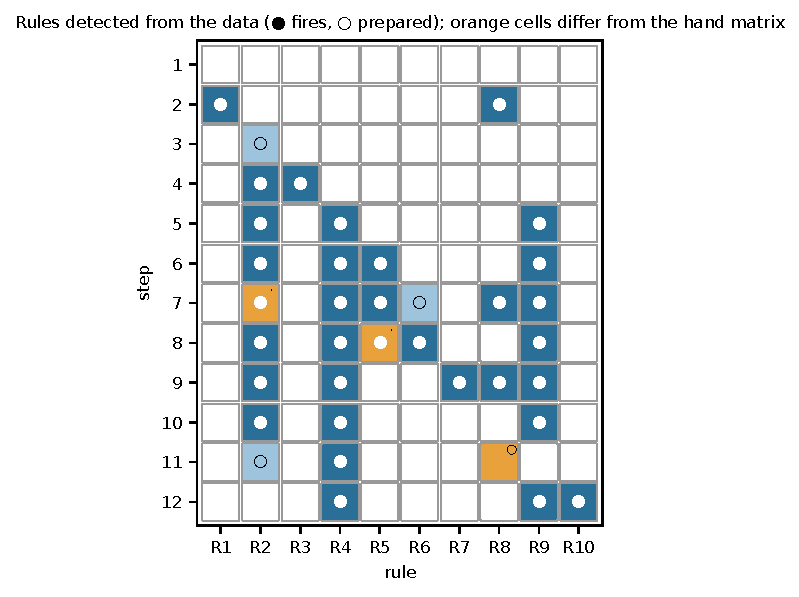
\includegraphics[width=0.62\textwidth]{fig_rule_matrix.pdf}
\caption{The detected rule matrix (orange: cells that differ from the hand matrix; the small symbol is the hand value).}\label{fig:rulematrix}
\end{figure}

\begin{proposition}[Rule detection]\label{prop:detection}
The predicates P1--P10 evaluated on the page view reproduce the hand-assigned rule matrix of the repository in \NhepAgree{} of its 120 cells and the ``where each rule fires'' table of the branch's paper in \NhepPaperAgree{} of 120 cells. The \NhepDisagree{} disagreements with the hand matrix are: (Step 7, R2) the engine fires R2 because the new contact node reaches the muon lifetime, an observable with badge A added in the same step, whereas the hand matrix leaves the cell empty although the paper's table lists Step 7 under R2; (Step 8, R5) the engine marks the merged V$-$A node effective because its coupling is dimensionful (kind \emph{eff}), whereas the hand matrix leaves the cell empty although the paper's table lists Step 8 under R5; (Step 11, R8) the hand matrix marks R8 as prepared because a massless neutrino representation cannot carry a mass difference, a statement about the content of the representation that no structural predicate sees.
\end{proposition}
\begin{proof}
By computation (\texttt{replay\_hep.py}, fields \texttt{comparison}); the three cells are listed in the output with the engine's and the hand value.
\end{proof}
Two of the three disagreements are thus inconsistencies between the two hand-made tables of the repository, which the automatic detection exposes. Read with a prepared mark counted as not firing, the page matrix and the paper's table disagree in eight cells: (2,R8), (8,R9) and (12,R9), where the matrix marks a firing the table omits (the partition as a change of the state layer; re-attached calibration edges), and (7,R2), (7,R6), (8,R5), (11,R2) and (11,R8), where the table lists a firing the matrix records as prepared or omits. The engine sides with the matrix in six of the eight (its predicates distinguish a firing from a preparation and count a re-attached calibration edge as a calibration), with the table in (7,R2) and (8,R5), and with neither in (11,R8). The third disagreement with the matrix is the one place in twelve steps where a rule's precondition is a fact about the physics of a node (a massless representation) rather than about the graph. This is a measurement of how mechanical the history is: \NhepAgree{} of 120 cells are decided by structure, and the one content-based cell is identified as such.

\section{Generation from the observables}
\begin{table}[htbp]\centering\footnotesize
\caption{The recorded driver of each step against the engine's reading of the observable layer: whether an unexplained observable exists before the step, and the form of R2 detected (anomaly: a deficit or a same-step observed-before-explained observable is reached by the new model node; theory-internal: no such observable; announced: a candidate node; flagged: a new deficit and no model node).}\label{tab:drivers}
\begin{tabular}{@{}rlllp{4cm}@{}}\toprule
Step & id & recorded driver & deficit before the step & R2 form detected \\\midrule
2 & wigner & symmetry (theory-internal) & no & -- \\
3 & anomaly & anomaly: observed, unexplained & no & flagged \\
4 & fock & model response to the anomaly & yes & anomaly \\
5 & qed & anomaly: observed, unexplained & yes & anomaly \\
6 & fermi & anomaly: observed, unexplained & yes & anomaly \\
7 & muon & anomaly: observed, unexplained & no & anomaly \\
8 & va & anomaly: observed, unexplained & no & theory-internal \\
9 & ew & prediction (theory-internal) & no & theory-internal \\
10 & higgs & prediction (theory-internal) & no & theory-internal \\
11 & frontier & anomaly: observed, unexplained & no & announced \\
12 & sm & synthesis & yes & -- \\
\bottomrule\end{tabular}

\end{table}
The history is driven by its observables, and \cref{tab:drivers} measures that statement. Each step of the data carries a hand-written \emph{driver} (foundation, symmetry, anomaly, response, prediction, synthesis); the engine reads the observable layer and classifies the model-layer change by R2 alone. The two agree step by step: the steps whose driver is \emph{anomaly} or \emph{response} are exactly the steps at which a deficit exists before the step or an observed-before-explained observable arrives with the node that explains it (Steps 4--7), the steps whose driver is \emph{prediction} are exactly the theory-internal firings (Steps 9, 10), the symmetry step (2) and the synthesis (12) add no interaction node, and the two steps with driver \emph{anomaly} that the engine classifies otherwise are the announcements (Step 3, a flag without a node; Step 11, a candidate node) and the V$-$A merge of Step 8, where the engine reads the parity observables as predictions of the merged node (badge P) rather than as a deficit. In this sense the historical graph is generated from clusters of observables: every interaction node is placed by an observable family (the $\sigma$- and $\Gamma$-type members of \cref{sec:families}) or by a symmetry requirement, and the engine locates which.

\section{Families and the cumulative deficit}
With the observable families of \cref{sec:families}, the cumulative deficit runs \NhepTrajUnexpCum{} over the twelve steps, against \NhepTrajUnexp{} in the page view (\cref{tab:steps}, \cref{fig:hep}). The two views agree on when a deficit opens (Steps 3, 11) and closes (Step 6, after the Fermi node reaches $\beta$ decay, the only $\Gamma$-type member then present), and the cumulative view adds the information that the $\sigma$-type family is closed at Step 5 by the first explicit cross sections while the $\Gamma$-type family stays open until Step 6. In the final cumulative graph \NhepUnexplainedFinal{} observable is unexplained (\NhepUnexplainedFinalList{}, neutrino flavour oscillation), the badges count \NhepBadgeA{} observed-before-explained, \NhepBadgeP{} predicted-before-observed and \NhepBadgeF{} calibrations, and \NhepMTwoOCumFinal{} model$\to$observable routes persist through the successor map. Without the family closure four observables would remain unexplained (the three generic heads and oscillation): the families are what the page means when it rewrites ``particle production'' into widths and cross sections, and the engine has to know it.

\section{Predictive content (Rule 9 on the final graph)}
\begin{table}[htbp]\centering\scriptsize
\caption{Rule 9 evaluated on the final cumulative graph: per surviving model node, the observables it predicts (an observable that calibrates the node is counted as a calibration, not a prediction), its calibrations and its framework assignments.}\label{tab:predictive}
\begin{tabular}{@{}lrrrp{6.2cm}p{2.6cm}@{}}\toprule
Node & predictions & calibrations & framework & predicted observables & calibrating observables \\\midrule
m\_field & 1 & 0 & 0 & o\_E &  \\
m\_A & 0 & 0 & 4 &  &  \\
m\_U & 2 & 0 & 0 & o\_m, o\_s &  \\
c\_gf & 15 & 3 & 0 & o\_ae, o\_beta, o\_compton, o\_hel, o\_lamb, o\_michel, o\_mutau, o\_mw, o\_mz, o\_nc, o\_nnu, o\_ntau, o\_pair, o\_twonu, o\_wu & o\_GF, o\_alpha, o\_sw \\
c\_gg & 1 & 0 & 0 & o\_tgc &  \\
c\_hg & 3 & 0 & 0 & o\_hbr, o\_mw, o\_mz &  \\
c\_yuk & 1 & 1 & 0 & o\_hbr & o\_mf \\
c\_pot & 1 & 1 & 0 & o\_lam & o\_mh \\
\bottomrule\end{tabular}

\end{table}
\Cref{tab:predictive} gives, for each surviving model node, its predicted and calibrating observables after the successor map has re-attached the routes of absorbed nodes. The gauge--fermion cluster predicts \NhepPCcgfpred{} observables with \NhepPCcgffit{} calibrations ($\alpha$, $G_F$, $\sin^2\theta_W$); the Yukawa cluster predicts the Higgs rates with the fermion masses as calibration; the potential predicts the self-coupling, untested, with $m_H$ as calibration; in all \NhepPCtotalPred{} predictions against \NhepPCtotalFit{} calibrations. This is the graph's statement of the predictive power of the electroweak theory: the excess of solid over dashed edges, computed rather than asserted.

\section{The sector--term census and the agenda of the history}
\begin{table}[htbp]\centering\small
\caption{Sector $\times$ term census of the final Standard Model graph: a filled cell means the sector is a leg of a route into the term.}\label{tab:sectorterm}
\begin{tabular}{@{}lcccccc@{}}\toprule
sector & c\_gf & c\_gg & c\_hg & c\_yuk & c\_pot & c\_bsm \\\midrule
s\_nue & $\blacksquare$ &  &  &  &  & $\blacksquare$ \\
s\_e & $\blacksquare$ &  &  & $\blacksquare$ &  &  \\
s\_num & $\blacksquare$ &  &  &  &  & $\blacksquare$ \\
s\_mu & $\blacksquare$ &  &  & $\blacksquare$ &  &  \\
s\_u & $\blacksquare$ &  &  & $\blacksquare$ &  &  \\
s\_d & $\blacksquare$ &  &  & $\blacksquare$ &  &  \\
s\_g & $\blacksquare$ & $\blacksquare$ &  &  &  &  \\
s\_W & $\blacksquare$ & $\blacksquare$ & $\blacksquare$ &  &  &  \\
s\_Z & $\blacksquare$ & $\blacksquare$ & $\blacksquare$ &  &  &  \\
s\_H &  &  & $\blacksquare$ & $\blacksquare$ & $\blacksquare$ & $\blacksquare$ \\
\bottomrule\end{tabular}

\end{table}
Rule R13 applied to the history takes the pair (sector, Lagrangian term) as its cell. \Cref{tab:sectorterm} shows \NhepSectorTermEntered{} of \NhepSectorTermCells{} cells filled. The empty cells are of two kinds: cells that the theory forbids (the photon and the gauge bosons do not enter the Yukawa term; the neutrinos, massless as drawn, do not enter it either) and cells that the drawing omits (the neutral-current route is drawn with one group leg over all fermions and the gauge self-interactions with the massive bosons only). The census does not know which is which; that is the content a solver adds. The agenda of the history is therefore: $U=\{$neutrino oscillation$\}$; $P=\{\lambda_{HHH}$, untested$\}$ together with the candidate neutrino-mass node and its candidate route; $Q=E=\emptyset$ (no shared calibration, no effective node survives); and \NhepSectorTermEmpty{} empty sector--term cells to be labelled forbidden or omitted. The first two items are exactly the frontier that the page marks; the third is what the uniform census adds.

%=====================================================================
\chapter{Regenerating the reading-indexed graphs}\label{ch:readers}

\section{Filtration}
\begin{proposition}[Filtration]\label{prop:filtration}
The electromagnetism reader (\NEMroutes{} routes over \NEMTimePoints{} paragraph indices up to \NEMTmax), the textbook reader (\NUProutes{} routes over \NUPTimePoints{} indices up to \NUPTmax) and the energy-flow network have no forward links: the numbers of routes that appear before one of their inputs or before their target are \NEMForwardLinks{}, \NUPForwardLinks{} and \NLGForwardLinks{}.
\end{proposition}
\begin{proof}
Exhaustive check of every route against the first-appearance index of its inputs and target (\texttt{filtration.py}).
\end{proof}
Rule R11 is thus satisfied by both texts. It is a non-trivial property of the writing: a textbook routinely uses a concept before it defines it, and the readers were written so that this never happens at the level of the graph.

\section{Failed routes and their resolution}
\begin{table}[htbp]\centering\scriptsize
\caption{Failed routes (Rule R12): the forward resolver is the first non-failed route into the same target at or after the failed route; the last column is the nearest non-failed route before it, usually the measurement the failed prediction is compared with.}\label{tab:failed}
\resizebox{\textwidth}{!}{\begin{tabular}{@{}lllllllll@{}}\toprule
Branch & failed route & target & $t$ & forward resolver & $t'$ & $t'-t$ & resolver kind & preceding route ($t$) \\\midrule
EM & g\_RJ & bbspec & 50 & g\_planckbb & 51 & 1 & quantization & -- (--) \\
EM & g\_photowave & photoel & 52 & g\_photoel & 52 & 0 & quantization & -- (--) \\
EM & g\_collapse & spectra & 53 & g\_bohrlines & 53 & 0 & quantum & -- (--) \\
EM & g\_diverge & lamb & 70 & g\_lamb & 73 & 3 & quantum & -- (--) \\
EM & g\_lambdirac & lamb & 70 & g\_lamb & 73 & 3 & quantum & -- (--) \\
EM & g\_ammdirac & amm & 70 & g\_amm & 73 & 3 & quantum & -- (--) \\
UP & r237 & CV & 270 & r484 & 575 & 305 & to\_classical & r236 (268) \\
UP & r412 & mmnull & 505 & -- & -- & -- & -- & r411 (504) \\
UP & r432 & bbrad & 521 & r434 & 523 & 2 & to\_classical & r430 (520) \\
UP & r438 & Kmax & 525 & r442 & 527 & 2 & to\_classical & r436 (524) \\
UP & r447 & Hspec & 531 & r450 & 534 & 3 & to\_classical & r445 (529) \\
UP & r470 & Ttun & 555 & -- & -- & -- & -- & r469 (554) \\
\bottomrule\end{tabular}
}
\end{table}
\Cref{tab:failed} lists the \NEMFailed{} failed routes of the history reader and the \NUPFailed{} of the textbook. In the history every failed classical prediction (Rayleigh--Jeans, the wave picture of the photoelectric effect, the collapsing atom, the divergent self-energy, the Dirac values of the Lamb shift and of the magnetic moment) is resolved by a quantisation or quantum route into the same target within \NEMFailedMaxDist{} paragraphs. In the textbook four of six failed routes are resolved forward, three of them within three paragraphs; the equipartition prediction of the heat capacity of hydrogen fails at paragraph 270 (volume 2, chapter 2) and is resolved only at paragraph 575, by the quantum freezing of degrees of freedom in the condensed-matter chapter of volume 3. The two unresolved cases are instructive: the ether prediction fails against the Michelson--Morley null result (the measurement route precedes it by one paragraph) and the resolution, special relativity, is added as a model node without a route back into the null-result node; the classical barrier is stated as failed one paragraph \emph{after} the quantum tunnelling route that resolves it. Both are properties of how the text was written, and the engine lists them because R12 asks for a forward route.

\section{Cycles and chains}
The 2-section of a reader (the digraph with an edge from every leg to its route's target) has \NEMEdgesTwosection{} edges for the history and \NUPEdgesTwosection{} for the textbook. It is not acyclic: the history has one strongly connected component of \NEMLargestSCC{} nodes, the textbook two components with \NUPNodesInCycles{} nodes in all (the larger of \NUPLargestSCC{}), the energy-flow network none. A representative cycle is force $\to$ state of motion $\to$ velocity $\to$ (with the magnetic field) force: observables and states determine each other in a loop, which is exactly the \emph{local cycle} the energy-flow branch studies in time. The filtration is nevertheless consistent, because the cycle closes across paragraphs (Newton's law at paragraph 2, the magnetic force at paragraph 18), and the longest chain of the condensed graph is \NEMLongestChain{} (history), \NUPLongestChain{} (textbook) and \NLGLongestChain{} (energy flow, acyclic). The hubs are states and models in the history (the gauge class of potentials, the state of motion, the Hilbert-space state) and laws and base quantities in the textbook (Newton's second law, mass, the time derivative and integral, current, temperature, Coulomb's law); the most frequent target in both is the force.

\begin{figure}[htbp]\centering
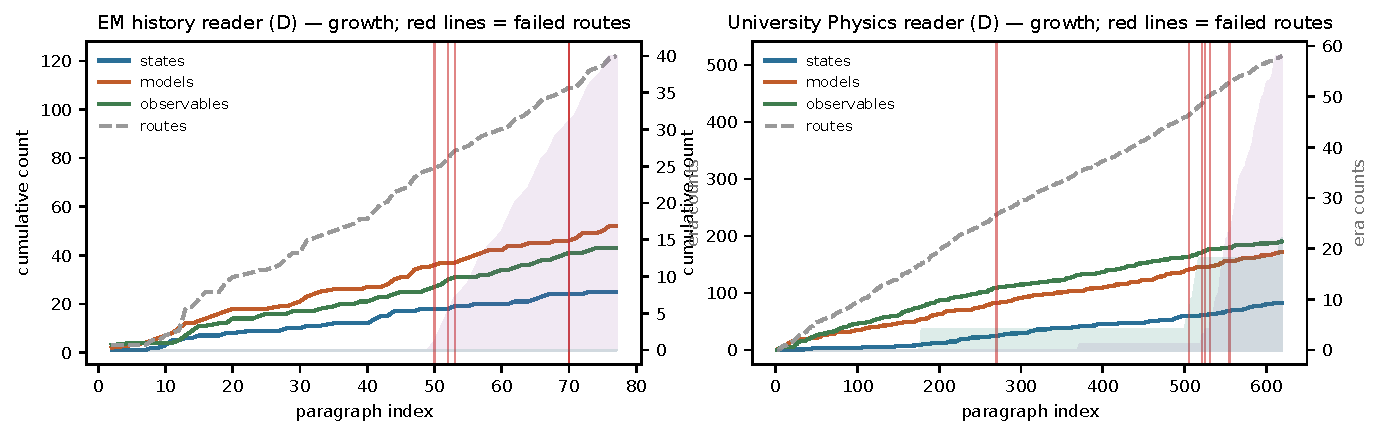
\includegraphics[width=\textwidth]{fig_growth.pdf}
\caption{Growth of the two readers with the paragraph index: cumulative states, models, observables and routes (left axis), quantum and relativistic nodes (right axis), failed routes (red lines).}\label{fig:growth}
\end{figure}
\Cref{fig:growth} shows the growth curves. Both readers grow almost linearly in the paragraph index with the observable layer ahead of the model layer and the state layer behind; the quantum nodes of the history enter at paragraph 50 and those of the textbook at paragraph 522 (one earlier quantum-era node, the superconducting state, is introduced in the chapter on current at paragraph 372), in both cases marked by a cluster of failed routes; the relativistic nodes of the textbook appear twice, with general relativity in the gravitation chapter (paragraph 177) and with special relativity in volume 3.

\section{The energy-flow branch}
The energy-flow network is the smallest branch (\NLGnodes{} nodes, \NLGroutes{} routes) and the one with the highest density of model nodes: nine of its model nodes are primitive (the field laws, the two parts of the lattice curl, the force coupling, the skew pairing, the energy form, the restriction to a region, the resistance), and every observable and state is derived from them by AND routes. Its four flow rules (conversion inside a region, conversion of field energy into matter energy, transport across the two boundaries) are glued in the grand network to Poynting's theorem of the history reader, and its four results (local observables cycle; the global observable is conserved; the local state wanders; the global state rotates) are the effect-type observables of a type D branch: claims about the behaviour of observables that the simulation establishes. The branch is acyclic as a graph; the cycles it studies are in the time evolution of its observables.

%=====================================================================
\chapter{Automatic exploration: census and closure}\label{ch:explore}

\section{The witness matrix of the nonclassicality network}
The nonclassicality network records, for each of its \NgptWitnesses{} witnesses, which state clusters and process clusters it requires and which it is blind to, and \NgptCombos{} combination records that give a verdict (fires, hidden, blind) for a (state, process) pair under several witnesses. The page computes from these a verdict for every cell of the witness $\times$ state $\times$ process matrix: the combination record if one exists, else blind if the state or the process is in the witness's blind list, else \emph{uncharted}. The engine implements the same rule and obtains \NgptSettled{} of \NgptCells{} cells settled (\NgptVerdictfires{} fires, \NgptVerdicthidden{} hidden, \NgptVerdictblind{} blind) and \NgptUncharted{} uncharted, the numbers the repository publishes for its version 2.6.
\begin{table}[htbp]\centering\small
\caption{Witness-matrix census per witness (182 cells each).}\label{tab:witness}
\begin{tabular}{@{}lrrrrr@{}}\toprule
Witness & settled & fires & hidden & blind & uncharted \\\midrule
w-bell & 31 & 3 & 0 & 28 & 151 \\
w-steer & 27 & 1 & 0 & 26 & 155 \\
w-incomp & 0 & 0 & 0 & 0 & 182 \\
w-entw & 29 & 2 & 1 & 26 & 153 \\
w-ncineq & 33 & 3 & 1 & 29 & 149 \\
w-sic & 30 & 2 & 0 & 28 & 152 \\
w-kcbs & 41 & 1 & 0 & 40 & 141 \\
w-wig & 39 & 0 & 0 & 39 & 143 \\
w-kd & 40 & 1 & 1 & 38 & 142 \\
w-weakval & 16 & 1 & 1 & 14 & 166 \\
w-workq & 40 & 1 & 1 & 38 & 142 \\
w-magicw & 51 & 2 & 0 & 49 & 131 \\
w-cohw & 52 & 0 & 2 & 50 & 130 \\
w-discw & 27 & 1 & 0 & 26 & 155 \\
w-clone & 13 & 0 & 0 & 13 & 169 \\
w-vis & 0 & 0 & 0 & 0 & 182 \\
w-sorkin & 0 & 0 & 0 & 0 & 182 \\
\bottomrule\end{tabular}

\end{table}
\begin{figure}[htbp]\centering
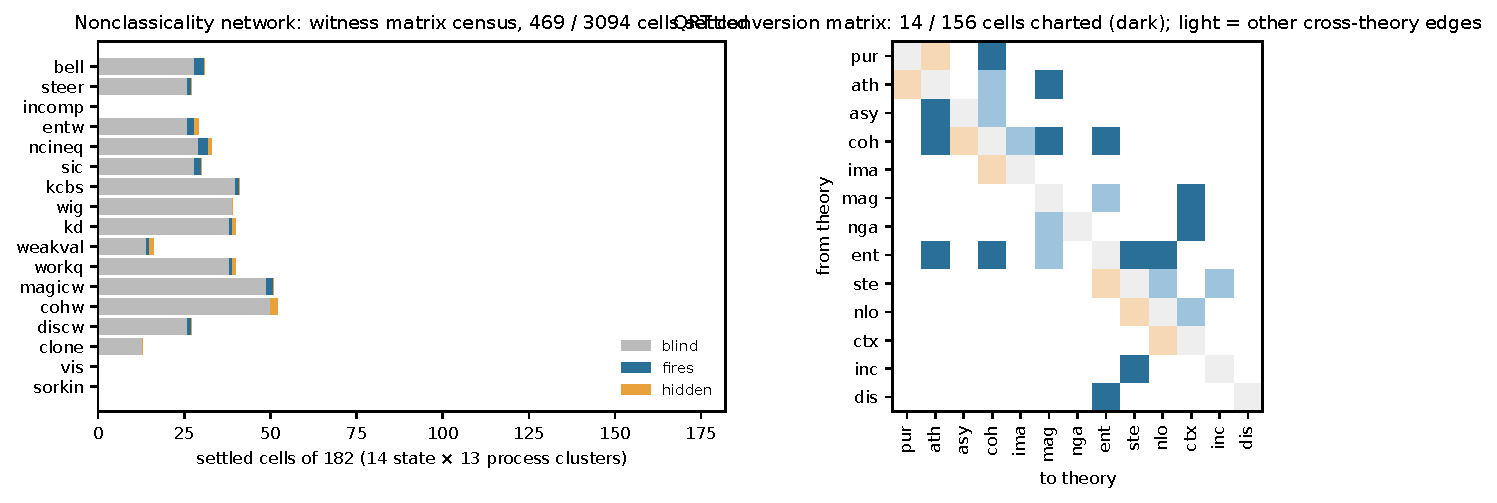
\includegraphics[width=\textwidth]{fig_census.pdf}
\caption{Left: settled cells per witness of the nonclassicality network. Right: the conversion matrix of the resource-theory network (dark: charted conversion cells; light: other cross-theory edges).}\label{fig:census}
\end{figure}
\Cref{tab:witness} and \cref{fig:census} show the census per witness. Three witnesses (joint-measurability SDP, fringe visibility, Sorkin $I_3$) have no settled cell at all; the magic and coherence witnesses have the most, because the round-4 results of the project recorded their blindness on covariant probes and on energy-diagonal states.

\section{The pair census}
The repository also counts node pairs: of \NgptPairs{} unordered pairs of the \NgptNodes{} nodes, \NgptConnectedPairs{} carry at least one edge and \NgptUnconnectedPairs{} do not; the \NGPTroutes{} edges are \NgptNoGo{} no-go, \NgptPossibility{} possibility or structure and \NgptOpen{} open. The engine reproduces these numbers. By native layer pair (\cref{app:pairs}) the census is far from uniform: nine layer pairs have no edge at all (axiom--process, axiom--witness, model--process, model--task, model--witness, process--witness, task--task, task--witness, witness--witness), while effect--effect, state--state and effect--state pairs are the densest (12/78, 13/91 and 15/182 pairs connected). The structural zeros are not gaps; they are the layer pairs the branch does not designate, and the designated pairs are the ones R13 enumerates. The uniform census over all pairs is therefore an overestimate of the research agenda by the undesignated pairs, and the engine reports the census per layer pair so that the designation can be read off.

\section{The conversion matrix of the resource-theory network}
\begin{table}[htbp]\centering\small
\caption{Conversion matrix of the thirteen resource theories ($\blacksquare$ charted by the repository's conversion group; $\square$ other state-to-state cross-theory edge; $\cdot$ other cross-theory edge).}\label{tab:qrt}
\resizebox{0.9\textwidth}{!}{\begin{tabular}{@{}lccccccccccccc@{}}\toprule
from $\backslash$ to & pur & ath & asy & coh & ima & mag & nga & ent & ste & nlo & ctx & inc & dis \\\midrule
pur & -- & $\cdot$ &  & $\blacksquare$ &  &  &  &  &  &  &  &  &  \\
ath & $\cdot$ & -- &  & $\square$ &  & $\blacksquare$ &  &  &  &  &  &  &  \\
asy &  & $\blacksquare$ & -- & $\square$ &  &  &  &  &  &  &  &  &  \\
coh &  & $\blacksquare$ & $\cdot$ & -- & $\square$ & $\blacksquare$ &  & $\blacksquare$ &  &  &  &  &  \\
ima &  &  &  & $\cdot$ & -- &  &  &  &  &  &  &  &  \\
mag &  &  &  &  &  & -- &  & $\square$ &  &  & $\blacksquare$ &  &  \\
nga &  &  &  &  &  & $\square$ & -- &  &  &  & $\blacksquare$ &  &  \\
ent &  & $\blacksquare$ &  & $\blacksquare$ &  & $\square$ &  & -- & $\blacksquare$ & $\blacksquare$ &  &  &  \\
ste &  &  &  &  &  &  &  & $\cdot$ & -- & $\square$ &  & $\square$ &  \\
nlo &  &  &  &  &  &  &  &  & $\cdot$ & -- & $\square$ &  &  \\
ctx &  &  &  &  &  &  &  &  &  & $\cdot$ & -- &  &  \\
inc &  &  &  &  &  &  &  &  & $\blacksquare$ &  &  & -- &  \\
dis &  &  &  &  &  &  &  & $\blacksquare$ &  &  &  &  & -- \\
\bottomrule\end{tabular}
}
\end{table}
The resource-theory network treats its $13\times 13$ matrix of ordered theory pairs (\NqrtCells{} off-diagonal cells) as its automation hook: a cell is charted when a conversion of one theory's resource into another's is recorded with the operation class under which it holds. The engine finds \NqrtCharted{} charted cells in the repository's conversion group (\cref{tab:qrt}), the number the repository publishes after its version 1.2 (the thermal-magic cell), and in addition \NqrtChartedStateState{} cells with some state-to-state cross-theory edge (set inclusions and memberships count here) and \NqrtCrossAny{} with any cross-theory edge. The \NqrtUncharted{} uncharted conversion cells are the branch's agenda; the \NqrtPartialEdges{} edges of status partial and the \NqrtGaps{} recorded gaps complete it.

\section{The record of closures}
The data contain the evidence that the loop of \cref{fig:cycle} has run. In the nonclassicality network the edge statuses are theorem (91), definition (22), derived (13), partial (11), open (10) and counterexample (9); the thirteen derived and nine counterexample edges are closures by elementary proof and by counterexample, and the edges whose statements begin with ``literature fill'' are closures by the fourth route. The eight edges of version 2.6 (U1--U7 and U5b) close two recorded gaps (SG1 at the level of models, SG5) and were generated from uncharted cells with the literature searched first; the seven edges of version 2.4 (R1--R6) were generated the same way one release earlier. In the resource-theory network the single edge of version 1.2 (C20) is a literature fill of a formerly uncharted conversion cell \citep{deoliveira2025}, and \NqrtGaps{} gaps are recorded. These are not claims of this thesis; they are the recorded history of two branches, read off their data, and they show the census and closure rules in operation.

\section{The same census on the other branches}
Applying R13 uniformly: for the history the cell is (sector, term), \cref{tab:sectorterm}; for the readers the natural cells are the primitive nodes (nodes with no route into them) and the OR targets (nodes with alternative derivations). The history reader has \NEMPrimitiveO{} primitive observable (\NEMPrimitiveOList), as its paper states, \NEMPrimitiveS{} primitive states and \NEMPrimitiveM{} primitive models; the textbook reader has \NUPPrimitiveO{} primitive observables (the base quantities and constants: \NUPPrimitiveOList), no primitive state and \NUPPrimitiveM{} primitive models. A primitive observable is a measurement with no derivation in the branch; the agenda of a reader is the list of these together with its failed routes without forward resolution (\cref{tab:failed}). The energy-flow branch has nine primitive models and nothing else primitive, as a simulation should.

%=====================================================================
\chapter{Pedagogical development}\label{ch:pedagogy}

\section{The textbook as a growing graph}
The textbook reader \citep{gen_learning}, written for the OpenStax text \citep{openstax_up}, grows by Rule R11 through \NUPChapters{} chapters. \Cref{fig:carryin} and \cref{app:chapters} give, per chapter, the new nodes, the routes and the \emph{carried-in} nodes: the nodes of earlier chapters that the chapter's routes connect to. The engine recomputes the carried-in counts from the routes and reproduces the per-chapter lists stored in the released file; across the book \NUPCarriedTotal{} carry-ins occur (a node is counted once per chapter it is carried into), with a maximum of \NUPCarriedMax{} in one chapter. The carry-in is what the page shows when the reader moves to a new chapter: only the earlier nodes that the chapter uses. It is a projection of the filtration, computable from the routes alone, and it is the pedagogical analogue of the cumulative view of the history: what the student must have in hand to read the chapter.
\begin{figure}[htbp]\centering
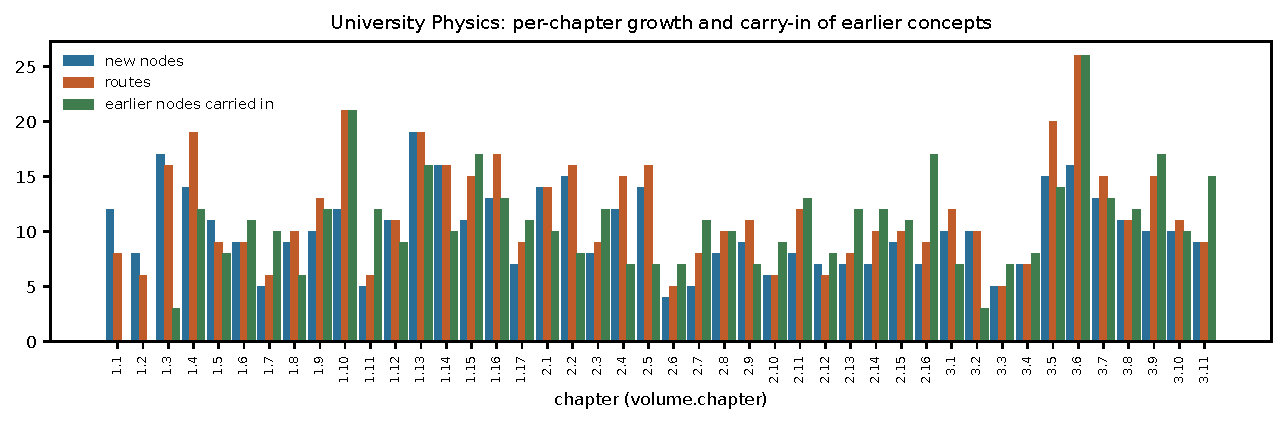
\includegraphics[width=\textwidth]{fig_carry_in.pdf}
\caption{Per-chapter growth of the textbook reader: new nodes, routes, and earlier nodes carried into the chapter by its routes.}\label{fig:carryin}
\end{figure}

\section{Historical versus pedagogical order}
\begin{figure}[htbp]\centering
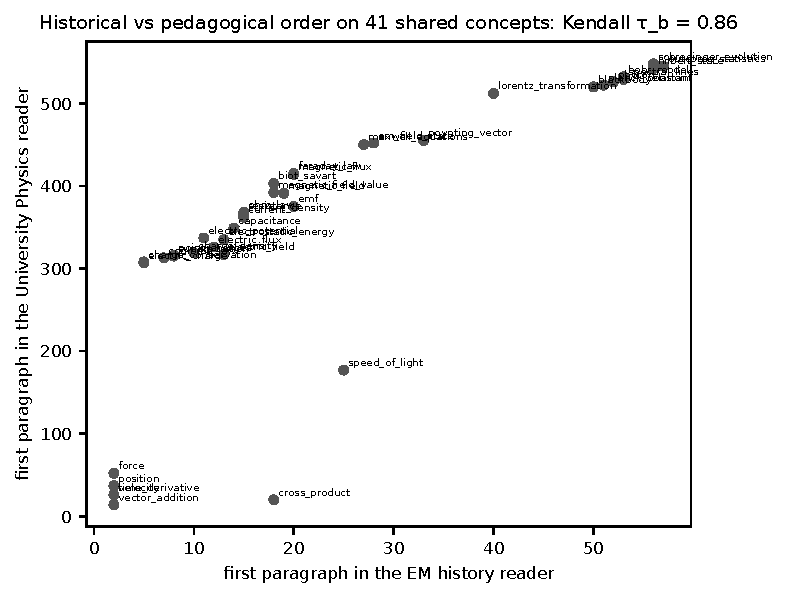
\includegraphics[width=0.62\textwidth]{fig_order.pdf}
\caption{First-appearance paragraph of the \NorderN{} concepts shared by the electromagnetism history reader and the textbook reader.}\label{fig:order}
\end{figure}
Two of the readers cover the same physics in two orders: the history reader in the order of discovery and the textbook in the order of teaching. On the \NorderN{} concepts they share (\cref{app:order}), the rank correlation of first appearance is Kendall $\tau_b=\NorderTau$ (Spearman $\rho=\NorderRho$), with \NorderConc{} concordant and \NorderDisc{} discordant pairs. The orders agree on the large scale (electrostatics, currents, magnetism, induction, Maxwell, relativity, quanta) and disagree in a few identifiable places: the cross product is a chapter-2 tool in the textbook and arrives with Ørsted and Ampère in the history; the speed of light is introduced with gravitation in the textbook (volume 1, chapter 13) and with the units of electromagnetism in the history; the electromotive force precedes the magnetic field in the textbook (circuits before magnetism) and follows it in the history (Faraday after Ørsted). The inversions are the places where teaching order departs from discovery order, listed mechanically.

\section{Role flips as a pedagogical signal}
Four of the \NnFlips{} role flips are between the two readers (blackbody radiation, a measured spectrum in the history and a state in the textbook; the photon; the Bohr model, orbits in one and postulates in the other; and, through the history of the Standard Model, hydrogen levels and decays). They mark the points where a textbook posits what history measured. A reader built from the grand network can show both: the measured spectrum that classical physics could not reproduce and the state that the textbook asks the student to accept, with the failed route between them.

%=====================================================================
\chapter{The methodology as an algorithm}\label{ch:algorithm}

\section{One step}
\begin{algorithm}[htbp]
\caption{\textsc{GenStep}: one step of the epistemic loop on a concept graph}\label{alg:step}
\KwIn{graph $G_t$ of a branch with conventions (type D/H/E, designated census pairs $\mathcal C$); an event $e$: a new observable node, a theorem, or the next paragraph of a text; a solver $\mathcal S$}
\KwOut{graph $G_{t+1}$, operation log $L$, agenda $A(G_{t+1})$}
place $e$ in its layer and sub-layer by the branch conventions; $G\gets G_t\cup\{e\}$\;
\If{$e$ is an observable with $N^-_{\lay M}(e)=\emptyset$}{\op{flag} $e$ (R2 precondition)\;}
\If{$e$ is a paragraph}{\op{add} its new nodes, \op{derive} its routes; check no forward links (R11); \op{fail} marked routes and record resolvers (R12)\;}
compute $U(G),Q(G),E(G),F(G),P(G)$ and the census $C(G)$ over $\mathcal C$ (\cref{thm:agenda})\;
\ForEach{enabled rule in R1--R10, R13}{
  \uIf{the rule needs content (R2 model node, R14 closure)}{ask $\mathcal S$ for a candidate; if none, record the cell as open\;}
  \Else{apply the operation; append to $L$ with the count deltas of \cref{tab:ops}\;}
}
check the invariants of the branch type (\cref{prop:discipline} for H; filtration for D; witness--effect pairing for E)\;
\Return $G_{t+1}=G$, $L$, $A(G_{t+1})$\;
\end{algorithm}
\Cref{alg:step} is the loop of \cref{fig:cycle} written as code. Lines 1--8 and 10--13 are executed by the engine; line 9 calls the solver. Everything in the instances that is logged (the operation logs of the Standard Model page, the version changelogs of the quantum networks, the paragraph markers of the readers) is the output $L$ of this step.

\section{What the solver must supply}\label{sec:solvers}
The solver is asked two kinds of question. For R2 it is asked for a model node that sends a route to the flagged observable and reproduces the routes of the node it replaces; R4 then reads the node's routes off its term, R5 marks its status from the dimension of its coupling, and R9 counts its calibrations. For R14 it is asked for the verdict of a cell: a composition of existing edges, an elementary proof, a counterexample, or a reference. The project has three solvers in use. The \emph{literature} is the solver of the quantum networks: every edge carries references, and a closure by literature fill is a search. A \emph{derivation} is the solver of the derived edges and of the propositions of the combined paper. An \emph{inference engine} is the solver of the project's two inverse-direction results, in the tradition of model learning from data \citep{brunton2016,wu2019,gentile2021}: the compose--modify--reduce engine, which on a simulated three-spin world with an impurity composed three spin-$\tfrac12$ sectors, tied the couplings by symmetry, reduced the representation by the commutant and predicted a neutron-scattering line before it was measured in the simulation; and TFO-Net, a factor-graph network that infers the operator content of a polynomial Lagrangian from response observables. Both engines answer R2 in the dynamic setting (which sector or term the data require), and both are instances of R15 and R16. The engine of this thesis does not run them; it locates where they are needed.

\section{Verification obligations}
A step is accepted when the new graph satisfies the invariants of its branch type: for type H, \cref{prop:discipline} and the rule that the state layer changes only from outside itself; for type D, the filtration property and the resolution of failed routes; for type E, the witness--effect pairing and the polarity convention. The engine checks them after every build; the counts in this thesis are the outcome of those checks on the released data.

%=====================================================================
\part{The evolution of the network}\label{part:evolution}
%=====================================================================
\chapter{Evolution of the effect and resource networks}\label{ch:evoE}

Part I treated the two quantum networks (GPT, QRT) as finished objects with a version axis, and the readers and the Standard Model history as graphs with a native time index (paragraph, step). This part puts all four on one calendar axis and derives how each grew, node by node and edge by edge. The quantum networks have no time axis of their own; what they have is a reference list on every edge, and on every node of the resource-theory network. The chronology below is computed from those references by rules stated once, and every number in this part is the output of \texttt{build\_evolution.py} on the same released data as Part I.

\section{A calendar axis from the references}\label{sec:dating}
\begin{definition}[year index of a type-E graph]\label{def:dating}
Let $G=(V,R)$ be an effect or resource network whose routes $r$ carry reference strings $\mathrm{refs}(r)$ and whose nodes may carry $\mathrm{refs}(v)$. For a reference string, its \emph{year} is the publication year in parentheses, or the year encoded in an arXiv identifier; a bare four-digit number placed like a page number is not a year. Then
\begin{itemize}[nosep]
\item $t(r)=\min\{\text{year of } s : s\in\mathrm{refs}(r)\}$: the earliest cited source (provenance \emph{cited});
\item $t(v)=\min\bigl(\{\text{year of } s: s\in\mathrm{refs}(v)\}\cup\{t(r): v\in r,\ t(r)\text{ defined}\}\bigr)$ (provenance \emph{node-ref} or \emph{edge});
\item $t(r)=\max\{t(u): u\in r\}$ if $r$ cites nothing dated (provenance \emph{propagated});
\item $t(v)=2026$ if no incident route and no node reference is dated (provenance \emph{project}).
\end{itemize}
A route whose references include a textbook or review phrase (``standard'', ``see'', ``review'') is flagged \emph{review-dated}. For the readers, $t$ of a paragraph is the first year mentioned in its text, carried forward within a section (fallback: the section's first year); a node is dated by its first paragraph and a route by $\max$ of its paragraph's year and its endpoints' years. For the Standard Model history, a node is dated by the first year of its \texttt{years} field (fallback: the start year of the first step that draws it) and a route by $\max$ of its step's start year and its endpoints' years.
\end{definition}

\begin{lemma}[the year index is a filtration]\label{lem:filtration}
Under \cref{def:dating}, $t(u)\le t(r)$ for every route $r$ and every endpoint $u\in r$ in all four branches.
\end{lemma}
\begin{proof}
For a type-E graph: a node dated by an incident route takes the minimum over its incident dated routes, hence $t(v)\le t(r)$ for every dated $r\ni v$; a node dated by its own reference is only earlier; a propagated route takes the maximum of its endpoints; a project-dated node has no dated incident route, so every route through it is propagated and dated $2026=t(v)$. For the readers and the history the route year is defined as a maximum that includes its endpoints. The engine asserts the inequality after dating; the count of violations is \EGPTForward{} (GPT) and \EQRTForward{} (QRT); for EM, \EemAdjusted{} of \EEMEfin{} routes and for HEP \EhepAdjusted{} of \EhepUnionRoutes{} routes had to be moved later than their paragraph or step year to satisfy it, which is the \emph{adjusted} provenance.
\end{proof}

\begin{table}[htbp]\centering\small
\caption{Provenance of the year index. Node years: \emph{edge} = earliest incident dated route; \emph{node-ref} = the node's own references (QRT); \emph{project} = no dated source, set to 2026; \emph{paragraph}/\emph{carried}/\emph{section} = the reader's text; \emph{node-years}/\emph{step} = the history's fields. Route years: \emph{cited}/\emph{review-dated}/\emph{propagated}; \emph{step+endpoints}, \emph{endpoints} = $\max$ rule.}\label{tab:evo_prov}
\begin{tabular}{@{}lp{5.6cm}p{6.2cm}@{}}\toprule
Branch & Node years (provenance: count) & Route years (provenance: count) \\\midrule
EM & carried 17, paragraph 102, section 1 & carried 13, paragraph 88, propagated 20, section 1 \\
HEP & node-years 76, step 2 & endpoints 24, step+endpoints 190 \\
GPT & edge 89, project 3 & cited 148, propagated 4, review-dated 4 \\
QRT & edge 19, node-ref 92, project 5 & cited 77, propagated 9 \\
\bottomrule\end{tabular}

\end{table}

\Cref{tab:evo_prov} gives the provenance counts. In the nonclassicality network \EGPTProvroutecited{} of \EGPTEfin{} routes are dated by a cited source and \EGPTProvnodeedge{} of \EGPTVfin{} nodes by an incident route; \EgptProjectNodes{} nodes carry no dated source (the unitary-dynamics, sharp-measurement and incompatible-set process nodes) and are placed at 2026. In the resource-theory network \EqrtNodeRef{} of \EQRTVfin{} nodes are dated by their own references and \EqrtProjectNodes{} are project-dated.

\section{What the years mean}\label{sec:dating-caveat}
The year index is an \emph{ingredient chronology}: a route is placed at the year of the oldest work it cites, which is the year from which its ingredients were available in print, not the year the route was established. The data cite sources selectively, so the ingredient year can precede the historical origin of a concept or follow it:
\begin{itemize}[nosep]
\item Bell nonlocality (\id{e-bell}) and its witness are dated 1969 because the route cites Clauser--Horne--Shimony--Holt \citep{chsh1969} and not Bell's 1964 paper \citep{bell1964}; Kochen--Specker contextuality (\id{e-ks}) is dated 1990 by Mermin \citep{mermin1990} rather than 1967 \citep{kochen1967}; entangled states (\id{s-ent}) are dated 1989 by Werner \citep{werner1989} rather than 1935 \citep{epr1935,schrodinger1935}; Wigner negativity (\id{s-wneg}) is dated 1946 by Groenewold \citep{groenewold1946} rather than 1932 \citep{wigner1932}, with Hudson's theorem \citep{hudson1974} among the later citations.
\item Conversely a route proved recently can be dated early by a background citation: the composed corollary \id{R3} (entangled states $\to$ generalised contextuality) cites Plávala--Gühne 2024 together with Werner 1989 and is dated 1989.
\end{itemize}
The ordering is therefore the ordering of the sources the networks' authors chose, and the thesis makes no historical claim beyond that. Two checks bound the effect of the convention. First, project-dated members are excluded from every lag statistic below and marked in the tables. Second, the whole analysis is recomputed with the \emph{latest} cited source as the route year (an upper bound on the establishment year) in \cref{tab:evo_robust}: node years move by \EGPTMaxShiftMean{} years on average in GPT (\EGPTMaxShiftZero{} of \EGPTVfin{} nodes unchanged) and by \EQRTMaxShiftMean{} years in QRT (\EQRTMaxShiftZero{} of \EQRTVfin{} unchanged); the closure fraction, the densification exponent and the preferential-closure ratio of \cref{ch:growth} change little (GPT: \EGPTClosureFrac\% $\to$ \EGPTMaxClosureFrac\%, $\alpha$ \EGPTAlpha{} $\to$ \EGPTMaxAlpha{}, ratio \EGPTPAratio{} $\to$ \EGPTMaxPAratio{}; QRT: \EQRTClosureFrac\% $\to$ \EQRTMaxClosureFrac\%, $\alpha$ \EQRTAlpha{} $\to$ \EQRTMaxAlpha{}, ratio \EQRTPAratio{} $\to$ \EQRTMaxPAratio{}), while the latencies shrink (GPT median \EGPTLatMedian{} $\to$ \EGPTMaxLatMedian{} years). The conclusions drawn below are the ones that survive this change.

\begin{table}[htbp]\centering\small
\caption{Robustness of the growth quantities of the effect networks to the dating convention: earliest cited source (the convention of this thesis) against latest cited source. Latency: median years between the later endpoint and the closure route. $\alpha$: densification exponent (\cref{sec:densification}). PA: preferential-closure ratio (\cref{sec:pa}).}\label{tab:evo_robust}
\begin{tabular}{@{}llrrrrrr@{}}\toprule
Branch & convention & first year & closure frac. & latency median & $\bar d_{\mathrm{arr}}$ & $\alpha$ & PA \\\midrule
GPT & earliest & \EGPTYZero{} & \EGPTClosureFrac\% & \EGPTLatMedian{} & \EGPTMeanArrDeg{} & \EGPTAlpha{} & \EGPTPAratio{} \\
GPT & latest & \EGPTMaxYZero{} & \EGPTMaxClosureFrac\% & \EGPTMaxLatMedian{} & \EGPTMaxMeanArrDeg{} & \EGPTMaxAlpha{} & \EGPTMaxPAratio{} \\
QRT & earliest & \EQRTYZero{} & \EQRTClosureFrac\% & \EQRTLatMedian{} & \EQRTMeanArrDeg{} & \EQRTAlpha{} & \EQRTPAratio{} \\
QRT & latest & \EQRTMaxYZero{} & \EQRTMaxClosureFrac\% & \EQRTMaxLatMedian{} & \EQRTMaxMeanArrDeg{} & \EQRTMaxAlpha{} & \EQRTMaxPAratio{} \\
\bottomrule\end{tabular}
\end{table}

\section{Arrivals and closures}\label{sec:arrivals}
\begin{definition}[arrival and closure]\label{def:arrival}
In a dated graph, a route $r$ is an \emph{arrival route} if at least one endpoint has $t(u)=t(r)$ (it is dated the year one of its nodes appears) and a \emph{closure route} if every endpoint satisfies $t(u)<t(r)$. The \emph{degree at arrival} of a node $v$ is $d_{\mathrm{arr}}(v)=|\{r\ni v: t(r)=t(v)\}|$. The \emph{latency} of a closure route is $t(r)-\max_{u\in r}t(u)$.
\end{definition}
The decomposition of a year's events into arrivals (nodes with the routes they bring) and closures (routes between nodes that were already present) is the temporal form of the distinction of Part I between the operations that add a node (\op{add}, \op{derive} with a new target, R2's new model node) and the operations that add a route only (R14 closure, R4 route, R9 calibration). \Cref{fig:evo_branches} shows the cumulative node counts by layer and the route counts of the four branches on the calendar axis; \cref{fig:evo_events} shows the yearly events of the two effect networks.

\begin{figure}[htbp]\centering
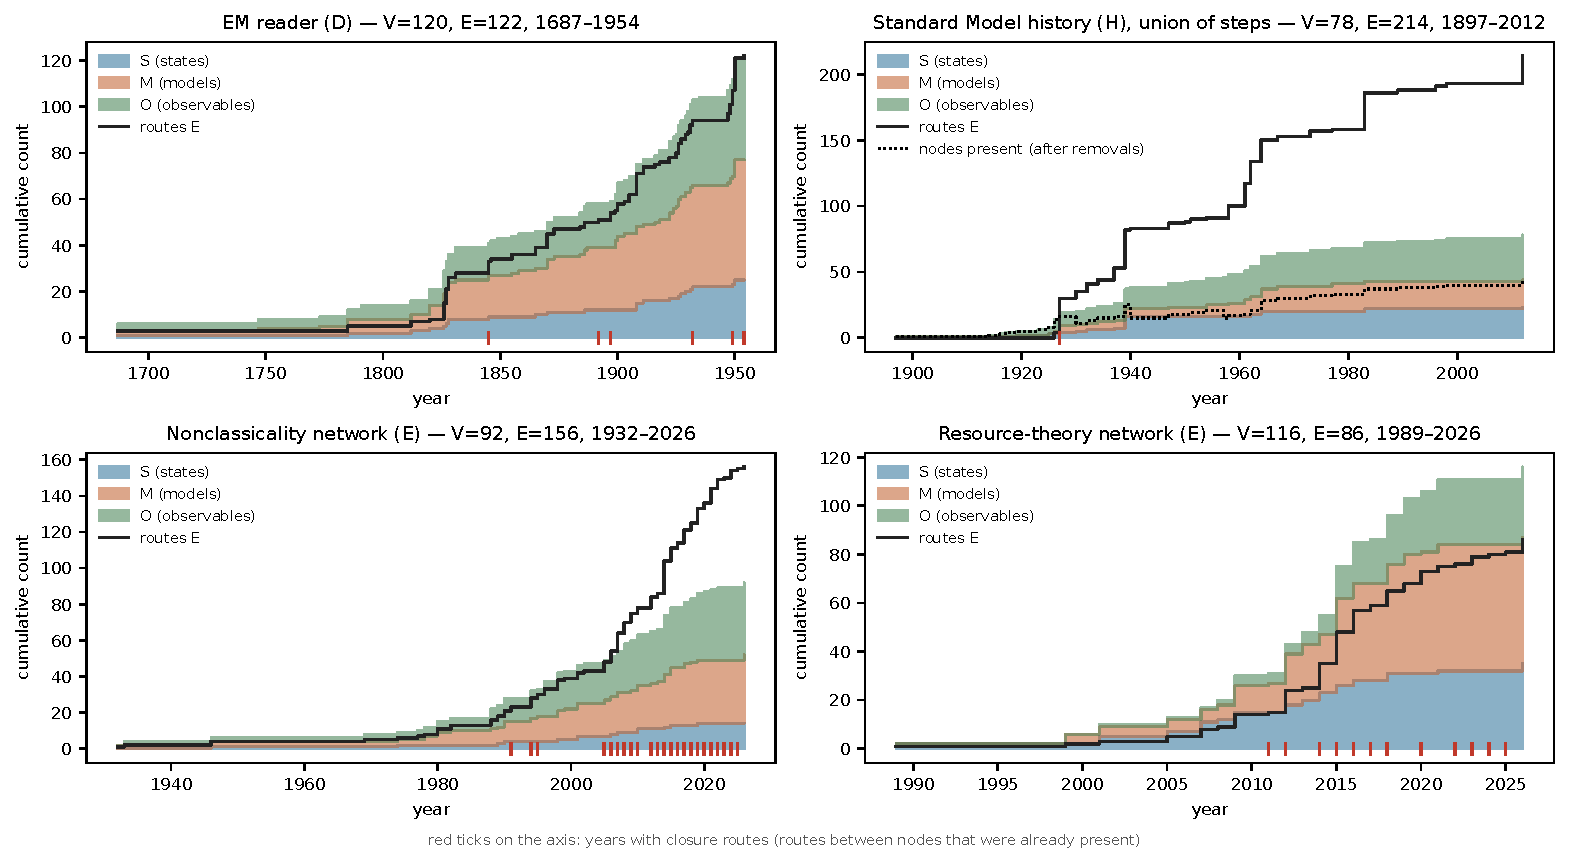
\includegraphics[width=\textwidth]{fig_evo_branches.pdf}
\caption{Cumulative node counts by layer (stacked) and route counts of the four branches on the calendar axis of \cref{def:dating}. Red ticks: years with closure routes. For the history the dotted line is the number of nodes present after removals (\cref{sec:removals}).}\label{fig:evo_branches}
\end{figure}

\begin{figure}[htbp]\centering
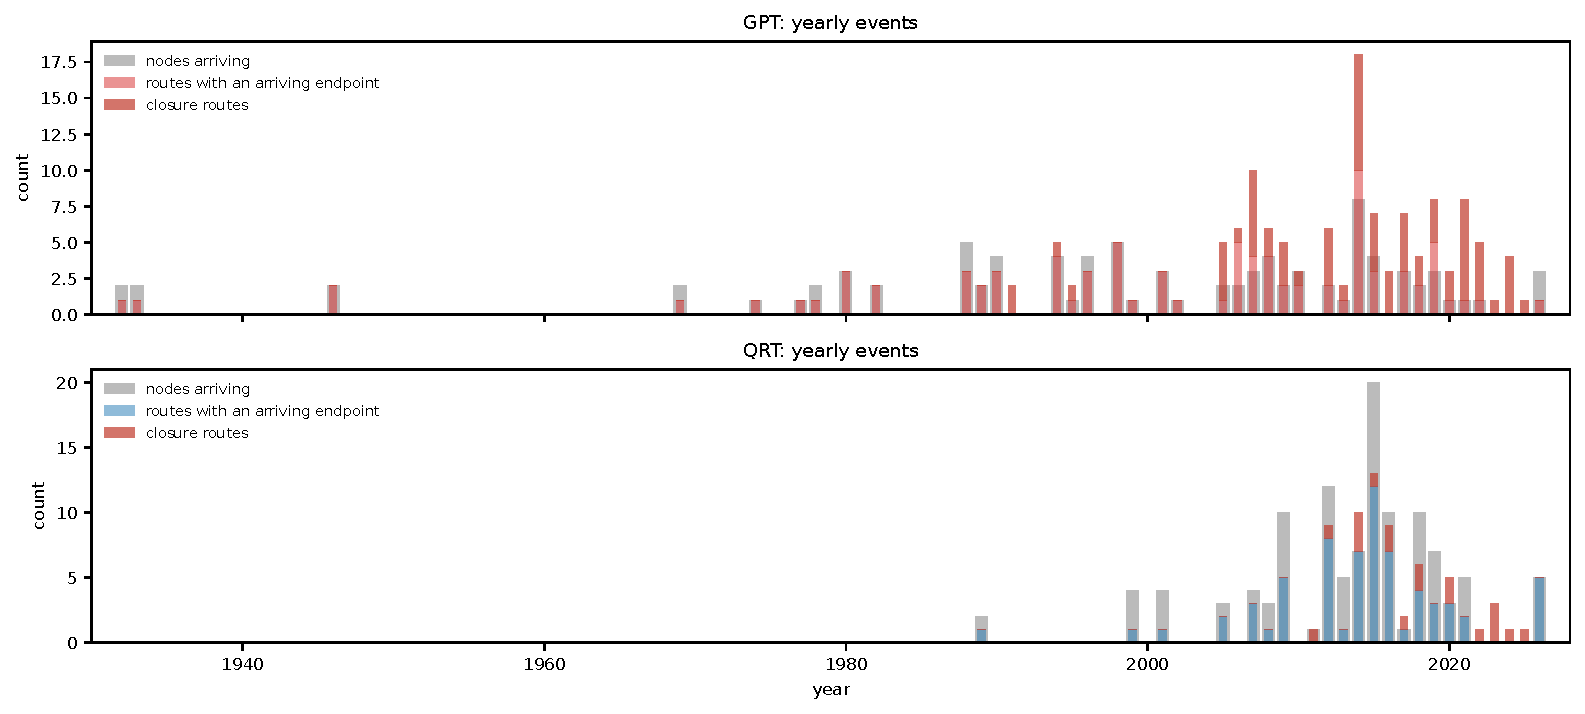
\includegraphics[width=\textwidth]{fig_evo_events.pdf}
\caption{Yearly events of the nonclassicality (GPT) and resource-theory (QRT) networks: nodes arriving, routes with an arriving endpoint, and closure routes.}\label{fig:evo_events}
\end{figure}

\subsection{The nonclassicality network}
The dated network starts with two nodes in \EGPTYZero{}: the complex-structure axiom and the quantum model (Stone's theorem, cited by \id{GN7}), then the Kirkwood--Dirac witness and effect (1933), the Moyal axiom and the Wigner-negative cluster (1946), the Bell witness and effect (1969), Gaussian states (1974) and the Wigner witness (1977). By 1950 the graph has \EGPTVAtOneNineFiveZero{} nodes and \EGPTEAtOneNineFiveZero{} routes, by 1980 \EGPTVAtOneNineEightZero{}/\EGPTEAtOneNineEightZero{}, by 1990 \EGPTVAtOneNineNineZero{}/\EGPTEAtOneNineNineZero{}, by 2000 \EGPTVAtTwoZeroZeroZero{}/\EGPTEAtTwoZeroZeroZero{}, by 2010 \EGPTVAtTwoZeroOneZero{}/\EGPTEAtTwoZeroOneZero{}, by 2020 \EGPTVAtTwoZeroTwoZero{}/\EGPTEAtTwoZeroTwoZero{}, and \EGPTVfin{}/\EGPTEfin{} at 2026. The route count overtakes the node count in \EGPTEoverV{} (\cref{fig:evo_branches}): \EGPTClosures{} of the \EGPTEfin{} routes (\EGPTClosureFrac\%) are closures, with mean latency \EGPTLatMean{} years, median \EGPTLatMedian{}, maximum \EGPTLatMax{}. This is the census-and-closure loop of \cref{ch:explore} seen in historical time: the cells of the witness matrix are opened by the arrival of witnesses and effects and are settled, on the median, fourteen years later. The per-year log of nodes and routes is \cref{app:events} (\cref{tab:evo_events_gpt}).

\paragraph{Witness before effect?} The \EgptPairs{} witness--effect pairs of the network (\cref{tab:evo_witness}) are dated the same year in \EgptPairsSame{} cases, the effect first in \EgptPairsEfirst{}, the witness first in \EgptPairsWfirst{}. Under the latest-source convention the counts are \EgptMaxPairsSame{}/\EgptMaxPairsEfirst{}/\EgptMaxPairsWfirst{}. In the data, therefore, a witness is never recorded before its effect except once, and most often the two appear in the same source: the effect is defined by the functional that detects it.

\paragraph{Explanation lag.} For each effect node, the years from its appearance to its first route from the model layer (\cref{tab:evo_explanation}): \EgptEffectsWithM{} of \EgptEffects{} effects have such a route, with mean lag \EgptLagMean{} years; \EgptLagZero{} are explained in their first year, Bell nonlocality waits \EgptLagBell{} years (\EgptBellYear{} to the first model route dated \EgptBellFirstM{}) and the Kirkwood--Dirac family \EgptLagKD{} years (\EgptKDYear{} to \EgptKDFirstM{}). The other \EgptEffectsNoM{} effects reach the model layer only through states or witnesses, which is the direct state--effect structure of type E (\cref{sec:contraction}).

\begin{table}[htbp]\centering\small
\caption{Witness--effect pairs of the nonclassicality network with the year of each member and of the pairing route.}\label{tab:evo_witness}
\begin{tabular}{@{}llrrrl@{}}\toprule
Witness & Effect & $t$(witness) & $t$(effect) & $t$(pair edge) & order \\\midrule
\texttt{w-bell} & \texttt{e-bell} & 1969 & 1969 & 1969 & same \\
\texttt{w-bell} & \texttt{e-pr} & 1969 & 1980 & 1994 & witness first \\
\texttt{w-steer} & \texttt{e-steer} & 2017 & 1998 & 2017 & effect first \\
\texttt{w-incomp} & \texttt{e-incomp} & 2019 & 1982 & 2019 & effect first \\
\texttt{w-entw} & \texttt{s-ent} & 1996 & 1989 & 1996 & effect first \\
\texttt{w-ncineq} & \texttt{e-ctx} & 2021 & 1989 & 2021 & effect first \\
\texttt{w-sic} & \texttt{e-ks} & 2008 & 1990 & 2008 & effect first \\
\texttt{w-kcbs} & \texttt{e-ksdep} & 2008 & 2008 & 2008 & same \\
\texttt{w-wig} & \texttt{s-wneg} & 1977 & 1946 & 1977 & effect first \\
\texttt{w-kd} & \texttt{e-kd} & 1933 & 1933 & 1933 & same \\
\texttt{w-weakval} & \texttt{e-weak} & 1988 & 1988 & 1988 & same \\
\texttt{w-workq} & \texttt{e-heat} & 2014 & 2014 & 2014 & same \\
\texttt{w-magicw} & \texttt{s-magic} & 2014 & 2001 & 2014 & effect first \\
\texttt{w-cohw} & \texttt{s-coh} & 2014 & 2007 & 2014 & effect first \\
\texttt{w-discw} & \texttt{s-discord} & 2008 & 2001 & 2008 & effect first \\
\texttt{w-clone} & \texttt{e-nobc} & 1996 & 1996 & 1996 & same \\
\texttt{w-vis} & \texttt{e-interf2} & 1988 & 1988 & 1988 & same \\
\texttt{w-sorkin} & \texttt{e-interf3} & 1994 & 1994 & 1994 & same \\
\bottomrule\end{tabular}

\end{table}

\begin{table}[htbp]\centering\small
\caption{Explanation lag of the effect nodes of the nonclassicality network: year of the effect, year of its first route from a model node and from a state node, and the lags.}\label{tab:evo_explanation}
\begin{tabular}{@{}lrrrrr@{}}\toprule
Effect & $t$(effect) & first M$\to$effect & lag (y) & first S$\to$effect & lag (y) \\\midrule
\texttt{e-kd} & 1933 & 1988 & 55 & 2021 & 88 \\
\texttt{e-bell} & 1969 & 1995 & 26 & 1989 & 20 \\
\texttt{e-pr} & 1980 & 1980 & 0 & -- & -- \\
\texttt{e-incomp} & 1982 & 1982 & 0 & -- & -- \\
\texttt{e-interf2} & 1988 & -- & -- & -- & -- \\
\texttt{e-weak} & 1988 & -- & -- & -- & -- \\
\texttt{e-ctx} & 1989 & 1990 & 1 & 1989 & 0 \\
\texttt{e-ks} & 1990 & -- & -- & 1990 & 0 \\
\texttt{e-interf3} & 1994 & 1994 & 0 & -- & -- \\
\texttt{e-nobc} & 1996 & -- & -- & 2008 & 12 \\
\texttt{e-steer} & 1998 & 1998 & 0 & -- & -- \\
\texttt{e-ksdep} & 2008 & -- & -- & 2014 & 6 \\
\texttt{e-heat} & 2014 & -- & -- & 2019 & 5 \\
\bottomrule\end{tabular}

\end{table}

\subsection{The resource-theory network}
The resource-theory network starts in \EQRTYZero{} with Werner's state and the nonlocality-free set, adds the convexity framework, discord (2001), magic (2005), entanglement and steering (2007) and the operation classes of 2009; the framework nodes (\id{F-QRT}, \id{F-TENSOR}) and five theories arrive in 2012, and the bulk of the network in 2014--2016 (by 2010 \EQRTVAtTwoZeroOneZero{} nodes, by 2015 \EQRTVAtTwoZeroOneFive{}, by 2020 \EQRTVAtTwoZeroTwoZero{}, \EQRTVfin{} at 2026). Here \EQRTClosures{} of \EQRTEfin{} routes (\EQRTClosureFrac\%) are closures with median latency \EQRTLatMedian{} years: the resource theories were connected to each other within a few years of being defined. The degree at arrival is low (\EQRTMeanArrDeg{} on average; \EQRTArrDegZero{} of \EQRTVfin{} nodes arrive with no route dated their own year), because a resource theory enters as a set of nodes (free set, resource set, operations, witness) whose routes are mostly the definitional ones that the data do not date and that the propagation rule places at the year of the latest endpoint.

\paragraph{The census in time.} \Cref{tab:evo_census} applies the pair census of \cref{ch:explore} to each year: the cells are the node pairs among the designated native-layer pairs (those that carry at least one edge in the final graph: \EgptDesignated{} pairs in GPT, \EqrtDesignated{} in QRT) restricted to the nodes present. The filled fraction of the nonclassicality network moves from \EGPTFilledRef\% in \EGPTFilledRefYear{} (\EGPTCellsRef{} cells) to \EGPTFilledLast\% in 2026 (\EgptCensusCellsFinal{} cells, a \EGPTCellsGrowth-fold growth); in the resource-theory network it falls from \EQRTFilledRef\% in \EQRTFilledRefYear{} to \EQRTFilledLast\% in 2026 (\EqrtCensusCellsFinal{} cells). The research front, measured as open cells, widens faster than it is filled, which is \cref{thm:agenda} read as a rate: the agenda grows quadratically in the node count while closures grow as $V^{\alpha}$ with $\alpha<2$ (\cref{sec:densification}).

\begin{table}[htbp]\centering\small
\caption{Pair census on the year axis: cells among present nodes in the designated layer pairs, connected cells, open cells and the filled fraction, at milestone years.}\label{tab:evo_census}
\begin{tabular}{@{}lrrrrr@{}}\toprule
Branch & Year & cells & connected & open & filled \\\midrule
GPT & 1990 & 295 & 21 & 274 & 7.1\% \\
GPT & 2005 & 868 & 45 & 823 & 5.2\% \\
GPT & 2010 & 1421 & 75 & 1346 & 5.3\% \\
GPT & 2015 & 2107 & 106 & 2001 & 5.0\% \\
GPT & 2020 & 2532 & 126 & 2406 & 5.0\% \\
GPT & 2026 & 2754 & 137 & 2617 & 5.0\% \\
QRT & 2005 & 78 & 5 & 73 & 6.4\% \\
QRT & 2015 & 2775 & 47 & 2728 & 1.7\% \\
QRT & 2020 & 5565 & 70 & 5495 & 1.3\% \\
QRT & 2026 & 6670 & 83 & 6587 & 1.2\% \\
\bottomrule\end{tabular}

\end{table}

\subsection{Polarity in time}
\Cref{fig:evo_polarity} separates the routes by polarity. The no-go routes of the nonclassicality network appear from \EGPTFirstNoGo{} and grow in step with the structural and possibility routes; in the resource-theory network the possibility routes (conversions, activations) dominate. \Cref{tab:evo_first_polarity} records, for each node, the polarity of its first incident route: \EgptMnoGoFirst{} of the \EgptMtotal{} model nodes of GPT enter through a pure no-go route and \EgptMnoGoAny{} through a first route that includes a no-go: a model (subtheory) is typically introduced by what it cannot do.

\begin{figure}[htbp]\centering
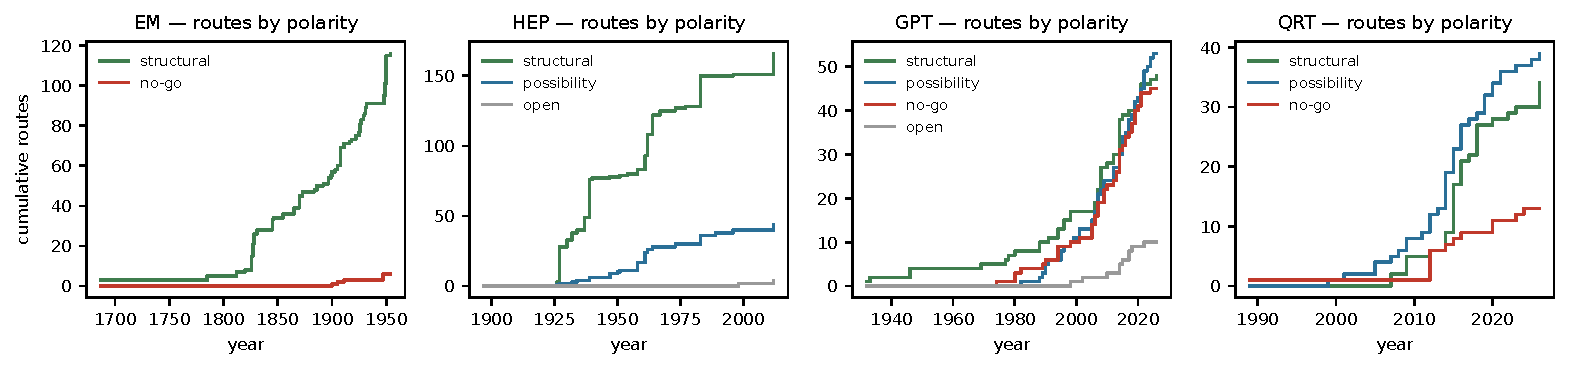
\includegraphics[width=\textwidth]{fig_evo_polarity.pdf}
\caption{Cumulative route counts by polarity. The reader's no-go routes are its failed derivations (R12); the history's possibility routes are its predictions and candidate routes; the effect networks separate structural, possibility and no-go closures.}\label{fig:evo_polarity}
\end{figure}

\begin{table}[htbp]\centering\small
\caption{Polarity of the first incident route of each node, by layer and branch (a node whose first routes have several polarities is counted under their combination; \emph{isolated} = no route).}\label{tab:evo_first_polarity}
\begin{tabular}{@{}l>{\raggedright\arraybackslash}p{3.6cm}>{\raggedright\arraybackslash}p{4.6cm}>{\raggedright\arraybackslash}p{4.2cm}@{}}\toprule
Branch & S nodes & M nodes & O nodes \\\midrule
EM & structural 24, no-go 1 (25) & structural 50, no-go 2 (52) & structural 38, no-go+\allowbreak{}structural 3, no-go 2 (43) \\
HEP & structural 22, open+\allowbreak{}structural 1 (23) & structural 12, possibility+\allowbreak{}structural 9 (21) & possibility 15, structural 14, possibility+\allowbreak{}structural 4, open 1 (34) \\
GPT & no-go 4, structural 3, no-go+\allowbreak{}possibility 2, no-go+\allowbreak{}structural 2, possibility 2, open+\allowbreak{}structural 1 (14) & no-go 17, structural 8, possibility 5, no-go+\allowbreak{}structural 2, no-go+\allowbreak{}possibility 2, isolated 2, no-go+\allowbreak{}possibility+\allowbreak{}structural 1, possibility+\allowbreak{}structural 1 (38) & structural 23, possibility 11, no-go 2, no-go+\allowbreak{}possibility 1, possibility+\allowbreak{}structural 1, no-go+\allowbreak{}structural 1, open 1 (40) \\
QRT & possibility 13, structural 12, isolated 3, no-go 3, possibility+\allowbreak{}structural 2, no-go+\allowbreak{}possibility+\allowbreak{}structural 1, no-go+\allowbreak{}structural 1 (35) & structural 20, possibility 11, isolated 9, no-go 8, no-go+\allowbreak{}structural 2, no-go+\allowbreak{}possibility 1, possibility+\allowbreak{}structural 1 (52) & possibility 14, isolated 13, structural 1, no-go 1 (29) \\
\bottomrule\end{tabular}

\end{table}

%=====================================================================
\chapter{The four-branch evolutionary network}\label{ch:merged}

\section{Construction}
\begin{definition}[evolutionary network]\label{def:merged}
Let $G_b$, $b\in\{\mathrm{EM},\mathrm{HEP},\mathrm{GPT},\mathrm{QRT}\}$, be the four dated graphs, where $G_{\mathrm{HEP}}$ is the \emph{union} of the twelve step graphs (every node and route that is drawn in any step, keyed by kind, inputs and target, dated at its first step and carrying the step at which it is last drawn), together with the observable-family, cluster-lineage and cluster-membership routes of the final view, dated at the year of their later endpoint. The evolutionary network at year $T$ is
\[ \mathcal G_T=\Bigl(\bigsqcup_b G_b\big|_{\le T}\Bigr)\cup\mathrm{Glue}_T, \]
where $G_b|_{\le T}$ keeps the nodes and routes with $t\le T$ (and, in HEP, drops an item once $T$ exceeds its removal year), and $\mathrm{Glue}_T$ contains, for each shared concept $c$ of the gluing catalogue (\cref{app:concepts}) with $k_c(T)\ge2$ members present, $k_c(T)-1$ identification edges joining its members in order of year. The \emph{collapsed} node count is $V^{\mathrm{col}}(T)=V(T)-\sum_c (k_c(T)-1)^+$, the number of nodes of the quotient of $\mathcal G_T$ by the identifications.
\end{definition}
\begin{lemma}\label{lem:collapse}
$V^{\mathrm{col}}(T)$ is the number of nodes of $\mathcal G_T/\!\sim$, where $u\sim v$ iff $u,v$ are members of the same concept, and $V^{\mathrm{col}}$ is non-decreasing in $T$ outside the HEP removal years.
\end{lemma}
\begin{proof}
The identification edges of a concept form a path on its $k_c$ present members, so the quotient merges them into one node and removes $k_c-1$ nodes; concepts are disjoint sets of members, so the removals add. Between removal years every term of $V(T)$ and every $k_c(T)$ is non-decreasing, and $V-\sum_c(k_c-1)^+=\sum_c 1+|\{v:\ v\text{ in no concept}\}|$ over present items is a count of present equivalence classes.
\end{proof}
The HEP union is the only non-monotone part of $\mathcal G_T$: \EhepRemovedNodes{} of its \EHEPVfin{} nodes and \EhepRemovedRoutes{} of its \EhepUnionRoutes{} routes are removed at some step (\cref{sec:removals}). A removal is placed at the start year of the removing step, never before the item's own year, and the final view (step 12, ``1927--2012'') places its removals at 2012. The merged curves of this chapter count ever-added items; the removal toggle of the explorer page and the dotted line of \cref{fig:evo_branches} apply the removals.

\section{Growth of the merged network}
\begin{figure}[htbp]\centering
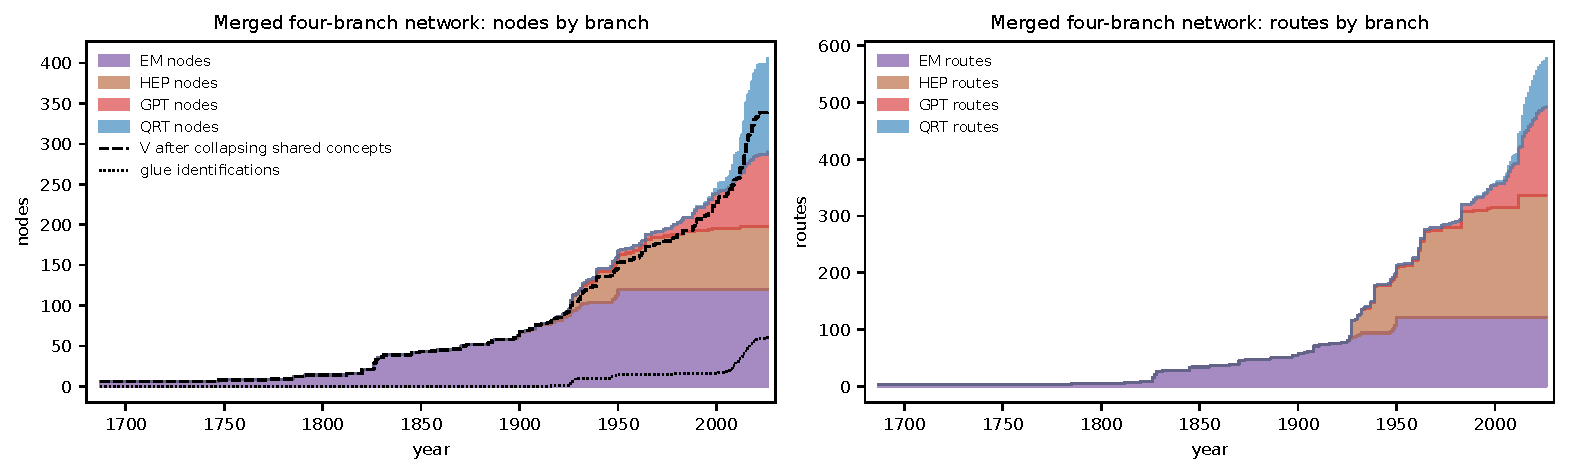
\includegraphics[width=\textwidth]{fig_evo_merged.pdf}\\[4pt]
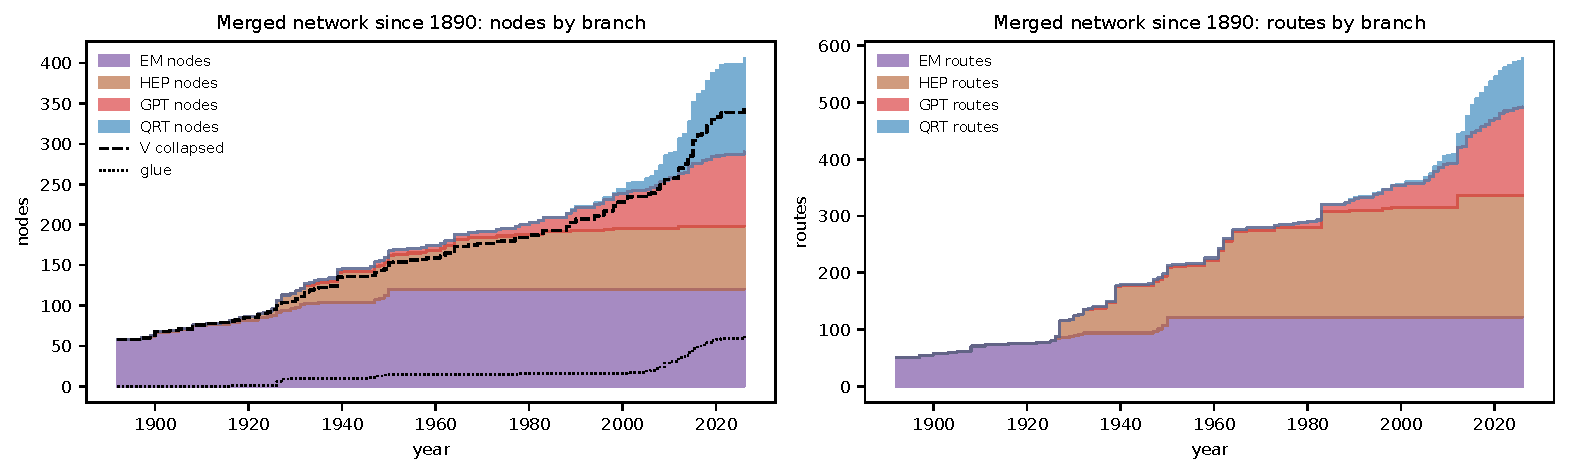
\includegraphics[width=\textwidth]{fig_evo_merged_zoom.pdf}
\caption{The evolutionary network: nodes (left) and routes (right) by branch, stacked, with the collapsed node count and the number of glue identifications; full axis above, from 1890 below.}\label{fig:evo_merged}
\end{figure}
At 1900 the evolutionary network has \EmergedVAtOneNineZeroZero{} nodes and \EmergedEAtOneNineZeroZero{} routes, all from the electromagnetism reader, and no glue; at 1950, \EmergedVAtOneNineFiveZero{} nodes, \EmergedEAtOneNineFiveZero{} routes and \EmergedGlueAtOneNineFiveZero{} identifications (the EM--HEP overlap of the 1920s--1940s: Lagrangian, photon, fine-structure constant, Lamb shift, anomalous moment); at 2000, \EmergedVAtTwoZeroZeroZero{}/\EmergedEAtTwoZeroZeroZero{}/\EmergedGlueAtTwoZeroZeroZero{}; at 2026, \EmergedV{} nodes (S \EmergedS{}, M \EmergedM{}, O \EmergedO{}), \EmergedE{} routes, \EmergedGlue{} identifications over \EnSharedFour{} shared concepts and \EmergedVcollapsed{} collapsed nodes. Half of the final node count is reached in \EmergedHalfYear{} and half of the final route count in \EmergedHalfYearE{}: the network of these four branches is, by count, a late-twentieth-century object, because the two effect networks are. \Cref{fig:evo_lanes} draws every node at its year in four lanes.

\begin{figure}[htbp]\centering
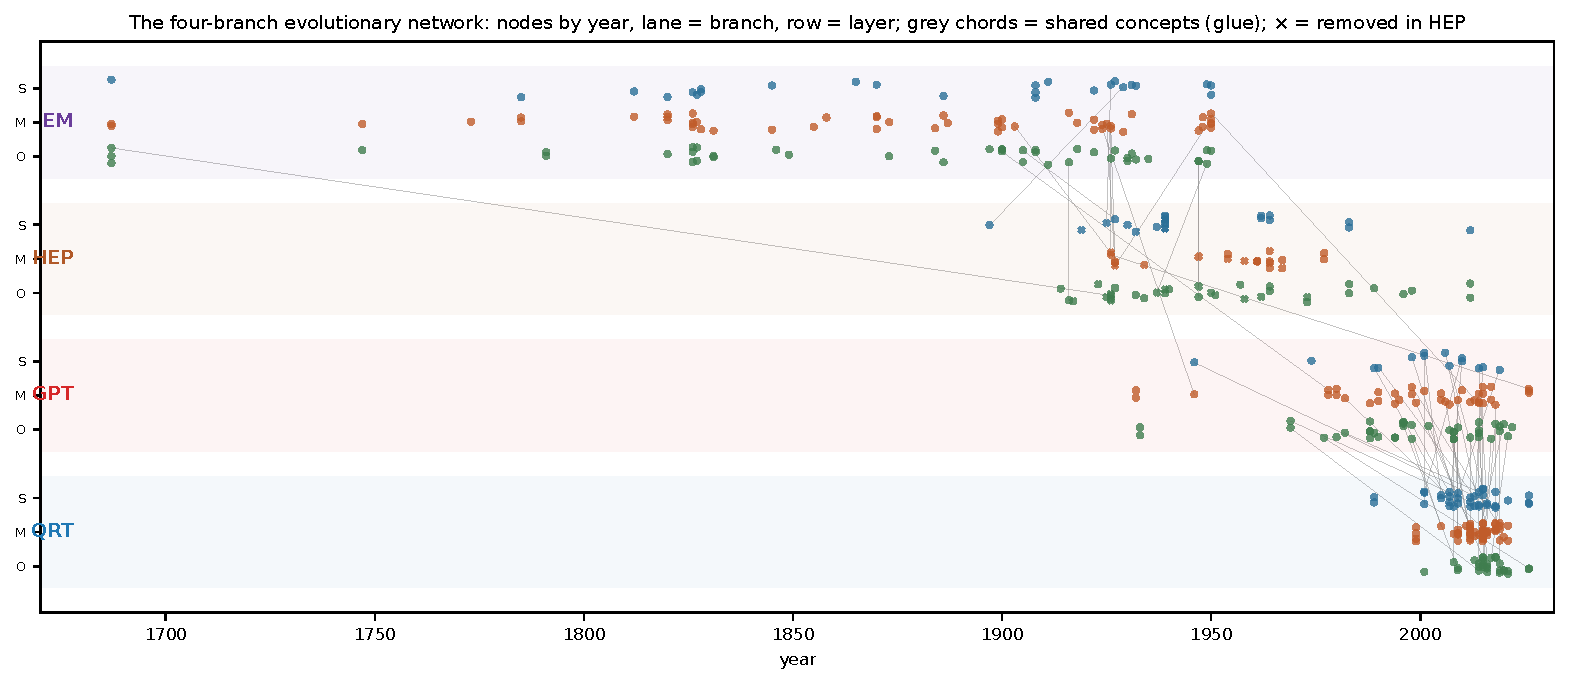
\includegraphics[width=\textwidth]{fig_evo_lanes.pdf}
\caption{Every node of the evolutionary network at its year (lane = branch, row = layer, colour = layer); grey chords join the members of shared concepts across branches; $\times$ marks nodes removed in the history.}\label{fig:evo_lanes}
\end{figure}

\section{Transfer between branches}\label{sec:transfer}
A shared concept has a year in each branch, and the \emph{lag} is the difference between the latest and earliest of them over its dated members (\cref{tab:evo_concepts_lag}, \cref{fig:evo_concepts}). Over the \EnSharedDated{} dated shared concepts the mean lag is \ElagMean{} years, the median \ElagMedian{}, \ElagZero{} are simultaneous and the maximum is \ElagMax{} (\ElagMaxLabel{}: \ElagMaxYears{}; in the history it is the position operator of one-particle quantum mechanics). The direction of transfer:
\begin{itemize}[nosep]
\item Between the two effect networks (\EnSharedGPTQRT{} shared concepts): GPT precedes QRT in \EfirstGPTamongGQ{} (mean lag \ElagGPTfirstMean{} years), QRT precedes in \EfirstQRTamongGQ{} (mean lag \ElagQRTfirstMean{} years), \EtieGQ{} are simultaneous. The dominant direction agrees with the contraction lemma of \cref{sec:contraction} read in time: an effect is named, witnessed and connected to subtheories before its state cluster is made the resource set of a resource theory.
\item Between the reader and the history (\EnSharedEMHEP{} shared concepts): EM first in \EfirstEMamongEH{}, HEP first in \EfirstHEPamongEH{}, \EtieEH{} simultaneous. The reader reaches the QED-era concepts (the electron field, the QED interaction, the cross section) later than the history dates them, because the reader's year is that of its paragraph while the history's is the node's own year field.
\end{itemize}
One shared concept (\EnSharedUndated{}) has a project-dated member in one branch and no dated lag. The lags inherit the ingredient-chronology caveat of \cref{sec:dating-caveat}; what the caveat cannot change is the simultaneous cases and the direction of a lag of a decade or more.

\begin{figure}[htbp]\centering
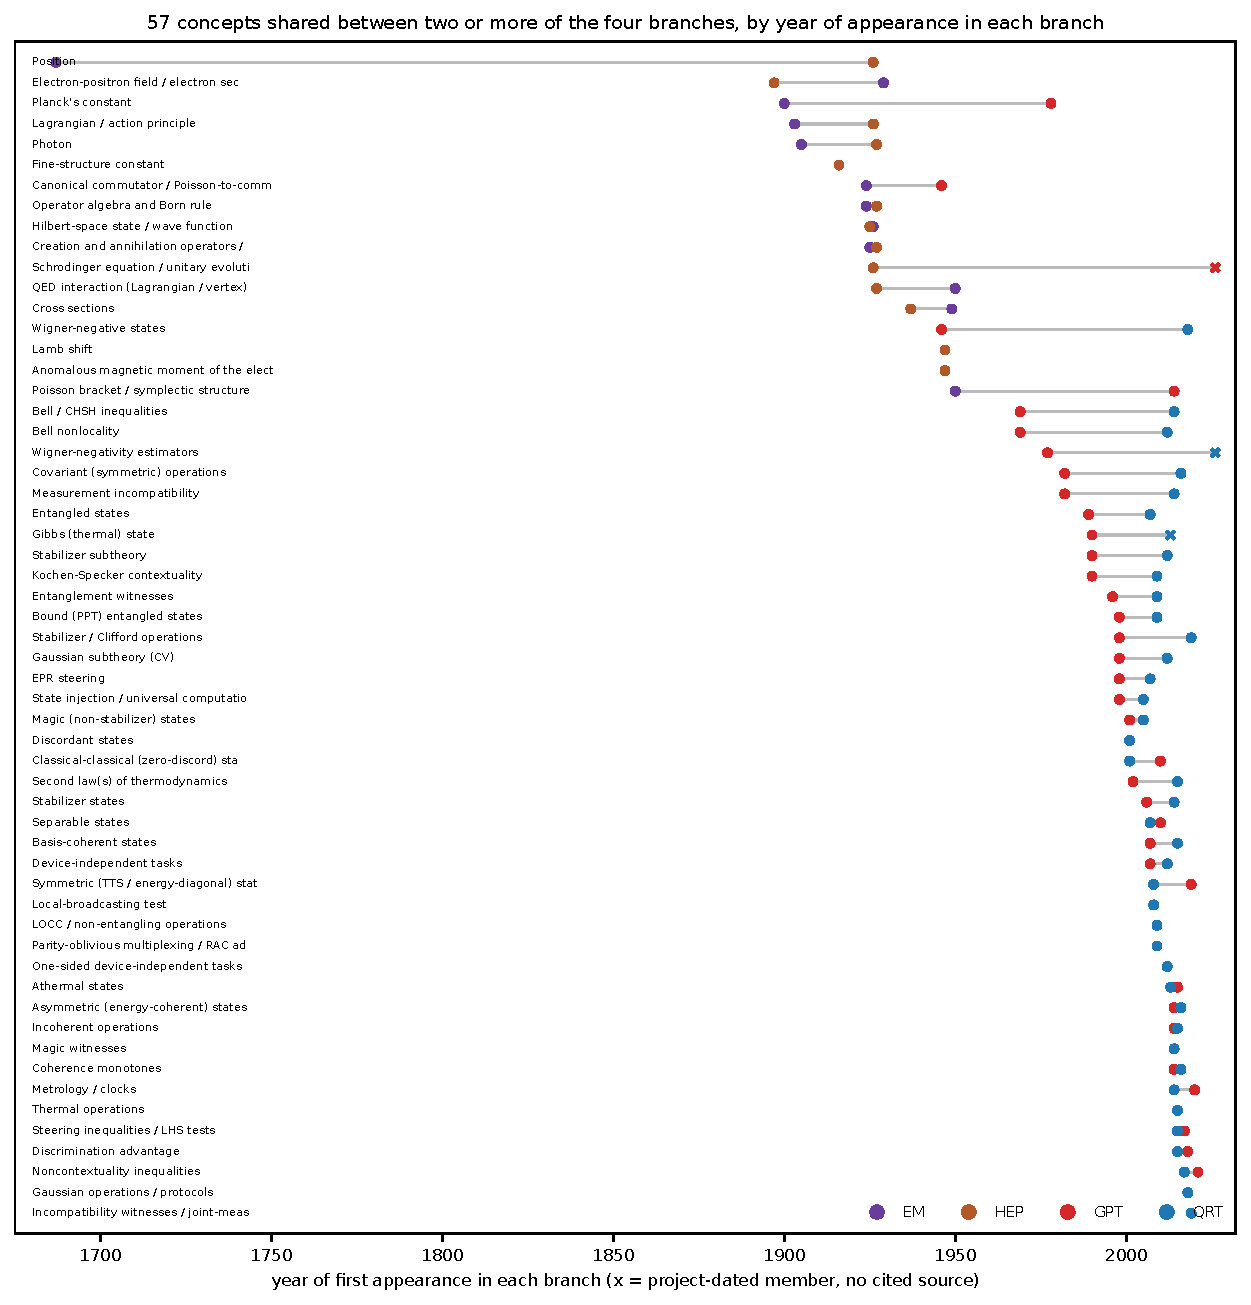
\includegraphics[width=\textwidth]{fig_evo_concepts.pdf}
\caption{The \EnSharedFour{} shared concepts of the four branches by year of first appearance in each branch (colour = branch; $\times$ = project-dated member).}\label{fig:evo_concepts}
\end{figure}

%=====================================================================
\chapter{Growth rules and counting identities}\label{ch:growth}

\section{The counting identity}
\begin{theorem}[arrival--closure identity]\label{thm:identity}
In a dated graph with $E$ routes, let $a(r)$ be the number of endpoints of $r$ with $t(u)=t(r)$, and let $C$ be the number of closure routes ($a(r)=0$). Then
\[ E=\sum_{v}d_{\mathrm{arr}}(v)-\sum_{r}\bigl(a(r)-1\bigr)^{+}+C . \]
\end{theorem}
\begin{proof}
$\sum_v d_{\mathrm{arr}}(v)=\sum_r a(r)$ by double counting the pairs $(v,r)$ with $v\in r$ and $t(v)=t(r)$. A route with $a(r)\ge1$ contributes $a(r)=1+(a(r)-1)^+$ to this sum and a route with $a(r)=0$ contributes $0$; so $\sum_r a(r)-\sum_r(a(r)-1)^+=|\{r:a(r)\ge1\}|=E-C$.
\end{proof}
The correction term is non-zero exactly for routes whose endpoints arrive together, which in a graph of directed hyperedges is common: a derivation of the reader that introduces its target together with one of its inputs, an \id{enters} route of the history dated with the sector it enters. \Cref{tab:evo_identity} verifies the identity on the four branches; it is the temporal counterpart of the count deltas of \cref{tab:ops}: every operation of Part I either adds a node with $d_{\mathrm{arr}}$ routes, adds a closure route, or removes.
\begin{table}[htbp]\centering\small
\caption{The arrival--closure identity of \cref{thm:identity} on the four dated branches.}\label{tab:evo_identity}
\begin{tabular}{@{}lrrrrrl@{}}\toprule
Branch & $\sum_v d_{\mathrm{arr}}(v)$ & $\sum_r (a(r)-1)^+$ & closures & $\sum_v d_{\mathrm{arr}} - \sum_r (a(r)-1)^+ + \text{closures}$ & $E$ & holds \\\midrule
EM & 174 & 60 & 8 & 122 & 122 & yes \\
HEP & 234 & 24 & 4 & 214 & 214 & yes \\
GPT & 110 & 23 & 69 & 156 & 156 & yes \\
QRT & 87 & 20 & 19 & 86 & 86 & yes \\
\bottomrule\end{tabular}

\end{table}

\begin{table}[htbp]\centering\small
\caption{Growth summary of the four dated branches. Frac.: closure fraction $C/E$. $\bar d_{\mathrm{arr}}$: mean degree at arrival. $\alpha$ ($R^2$): densification fit $\log E=\alpha\log V+c$ over the filtration years with $V\ge10$. PA ratio: mean degree of the endpoints of closure routes over the mean degree of all nodes present, evaluated before each closure ($n$ = number of closures).}\label{tab:evo_summary}
\resizebox{\textwidth}{!}{\begin{tabular}{@{}llrrrrrlrll@{}}\toprule
Branch & Years & $V$ & S/M/O & $E$ & Closures & Frac. & Latency mean/med/max (y) & $\bar d_{\mathrm{arr}}$ & $\alpha$ ($R^2$) & PA ratio ($n$) \\\midrule
EM & 1687--1954 & 120 & 25/52/43 & 122 & 8 & 7\% & 23.8 / 17 / 77 & 1.45 & 1.40 (0.98) & 1.16 (8) \\
HEP & 1897--2012 & 78 & 23/21/34 & 214 & 4 & 2\% & 1.0 / 1 / 1 & 3.00 & 1.62 (0.87) & 3.56 (4) \\
GPT & 1932--2026 & 92 & 14/38/40 & 156 & 69 & 44\% & 15.7 / 14 / 41 & 1.20 & 1.47 (0.99) & 2.86 (69) \\
QRT & 1989--2026 & 116 & 35/52/29 & 86 & 19 & 22\% & 4.1 / 4 / 12 & 0.75 & 1.30 (1.00) & 1.71 (19) \\
\bottomrule\end{tabular}
}
\end{table}

\section{Arrival degree and closure latency}
\Cref{tab:evo_summary} collects the quantities per branch. The mean degree at arrival separates the branch types: the history's nodes arrive with \EHEPMeanArrDeg{} routes each (a new sector enters its model and its observables in the same step), the reader's with \EEMMeanArrDeg{}, the effect networks' with \EGPTMeanArrDeg{} and \EQRTMeanArrDeg{}. The closure fraction is the complementary quantity: \EEMClosureFrac\% in the reader, \EHEPClosureFrac\% in the history, \EGPTClosureFrac\% and \EQRTClosureFrac\% in the effect networks. The readers and the history are \emph{arrival-driven}: a route almost always enters with a node, because a paragraph derives a new result and a step draws a new sector. The effect networks are \emph{closure-driven} to a large degree: their routes are theorems between existing nodes. \Cref{fig:evo_latency} gives the latency distributions: the reader's \EEMClosures{} closures have mean latency \EEMLatMean{} years (the two longest, \EEMLatSecond{} and \EEMLatMax{} years, are the Lorentz-force derivations of the 1890s between charge, force and field nodes of the 1820s), the history's \EHEPClosures{} closures have latency \EHEPLatMean{}, the effect networks' \EGPTLatMean{} and \EQRTLatMean{}.
\begin{figure}[htbp]\centering
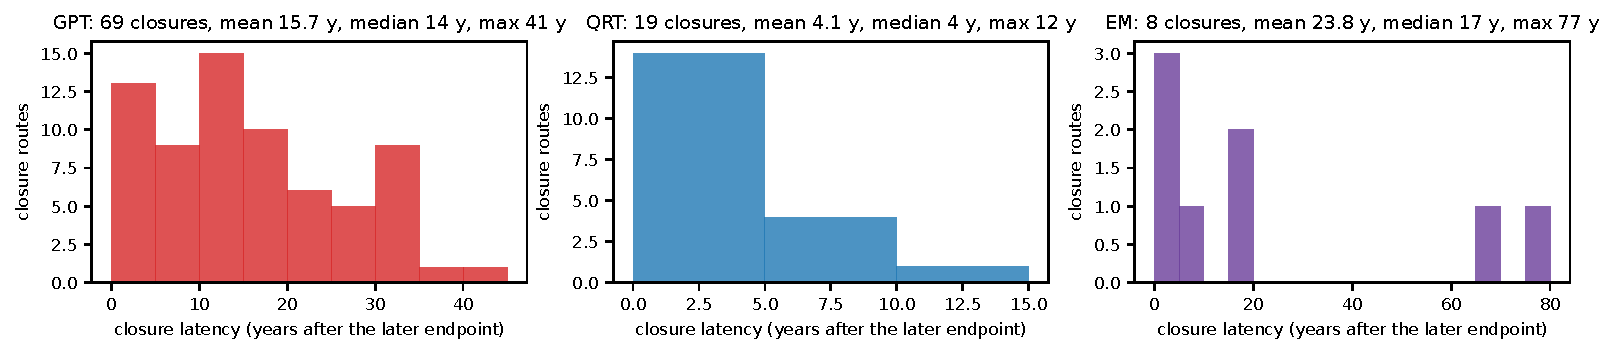
\includegraphics[width=\textwidth]{fig_evo_latency.pdf}
\caption{Closure latency (years from the later endpoint to the closure route) in the three branches with more than four closures.}\label{fig:evo_latency}
\end{figure}

\section{Preferential closure}\label{sec:pa}
For each closure route, the engine compares the mean degree of its endpoints at that time with the mean degree of all nodes then present; the ratio of the two sums over all closures is the \emph{preferential-closure ratio}, a discrete form of the attachment-kernel test of preferential-attachment models \citep{barabasi1999,newman2001}. It is \EGPTPAratio{} in GPT (\EGPTPAn{} closures), \EQRTPAratio{} in QRT (\EQRTPAn{}), \EEMPAratio{} in EM (\EEMPAn{}); the history has \EHEPPAn{} closures and the ratio is not meaningful. Closures attach to the best-connected nodes present: in the nonclassicality network the endpoints of a closing theorem have almost three times the mean degree. This is the behaviour of the census loop when the solver is the literature: the cells adjacent to well-studied nodes (Bell nonlocality, entanglement, Wigner negativity) are the ones for which a theorem is found.

\section{Densification}\label{sec:densification}
On the year filtration the route count grows faster than the node count. Fitting $\log E(T)=\alpha\log V(T)+c$ over the filtration years with $V(T)\ge10$ (\cref{fig:evo_densification}) gives $\alpha=\EEMAlpha{}$ ($R^2=\EEMAlphaR$) for the reader, \EHEPAlpha{} (\EHEPAlphaR) for the history, \EGPTAlpha{} (\EGPTAlphaR) for the nonclassicality network and \EQRTAlpha{} (\EQRTAlphaR) for the resource-theory network. Exponents between 1 and 2 are the densification power law observed in citation and collaboration graphs \citep{leskovec2007}; here they hold for concept graphs whose edges are mathematical relations, and they are stable under the dating convention (\cref{tab:evo_robust}). The right panel of \cref{fig:evo_densification} shows the degree-at-arrival distributions.
\begin{figure}[htbp]\centering
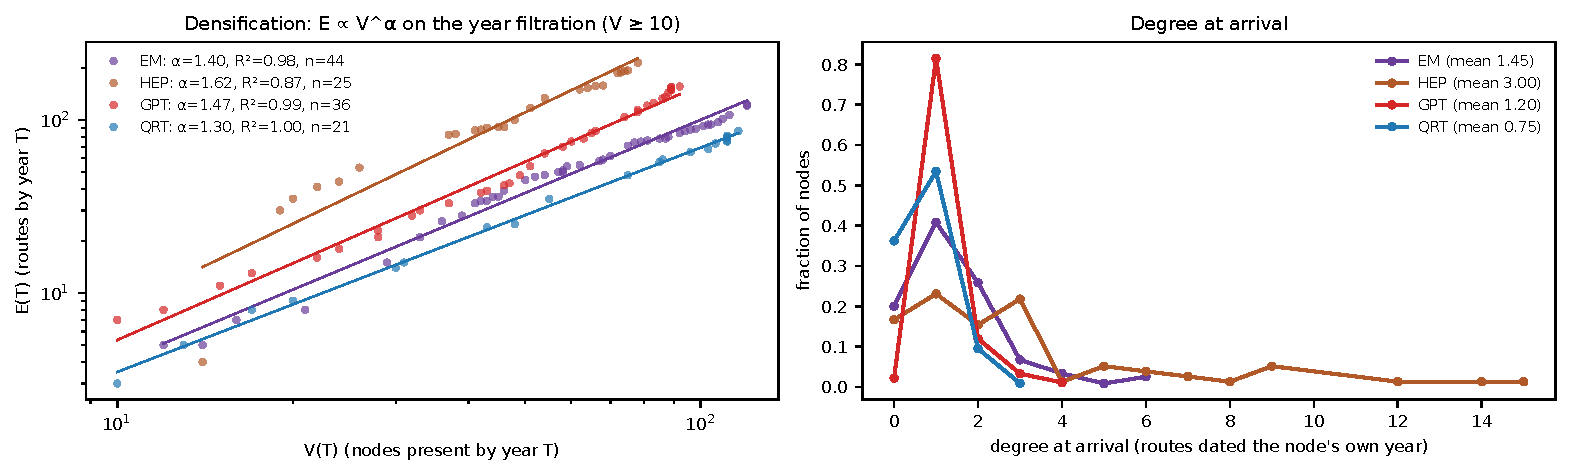
\includegraphics[width=\textwidth]{fig_evo_densification.pdf}
\caption{Left: $E(T)$ against $V(T)$ on the year filtration (log--log) with the fitted power laws. Right: distribution of the degree at arrival.}\label{fig:evo_densification}
\end{figure}

\section{Removals: the history as the only non-monotone branch}\label{sec:removals}
The reader and the two effect networks are filtrations: nothing is removed. The Standard Model history removes. \Cref{tab:evo_hep_removals} and \cref{fig:evo_hep_removals} count, per step, the nodes and routes added and removed in the union graph: \EhepRemovedNodes{} of \EHEPVfin{} nodes and \EhepRemovedRoutes{} of \EhepUnionRoutes{} routes. By sub-layer, the removed nodes are \EhepOdirectRemoved{} of \EhepOdirectAll{} direct observables (an observable is drawn in the step that explains it and dropped from the next drawing), \EhepSuirRemoved{} of \EhepSuirAll{} unitary-irreducible-representation state nodes (the Wigner classification of step 2, re-partitioned into Fock space and sectors at step 4), \EhepMfundRemoved{} of \EhepMfundAll{} fundamental model nodes (absorbed into the Lagrangian clusters of the final view), \EhepMeffRemoved{} of \EhepMeffAll{} effective models and \EhepMcandRemoved{} of \EhepMcandAll{} candidate (Fermi, muon and $V\!-\!A$ contact terms absorbed by their successors, R7/R10), \EhepSsectorRemoved{} of \EhepSsectorAll{} sectors and \EhepMframeRemoved{} of \EhepMframeAll{} frames; the \EhepMclusterAll{} cluster nodes are never removed. Removal in the history is of two kinds that the data distinguish: \emph{absorption}, where a lineage or back-edge names the successor, and \emph{de-selection}, where the page stops drawing an observable that is still explained. Only the first changes the state of knowledge; the cumulative view of \cref{ch:hep} keeps de-selected observables, and \cref{def:merged} keeps both with their removal step so that either reading can be reconstructed.
\begin{table}[htbp]\centering\small
\caption{Additions and removals per step of the Standard Model history (union graph).}\label{tab:evo_hep_removals}
\resizebox{\textwidth}{!}{\begin{tabular}{@{}lrrrrp{6.2cm}@{}}\toprule
Step & nodes added & routes added & nodes removed & routes removed & nodes removed (native ids) \\\midrule
1 & 9 & 9 & 0 & 0 &  \\
2 & 11 & 29 & 2 & 4 & H1, o\_x \\
3 & 1 & 0 & 1 & 1 & o\_L \\
4 & 8 & 37 & 14 & 31 & m\_L, o\_E, o\_p, o\_S, u\_vac, u\_m0, u\_mh, u\_m1, u\_0h, u\_01, u\_02, u\_cs, u\_tach, o\_prod \\
5 & 7 & 6 & 4 & 4 & o\_m, o\_s, o\_G, o\_sig \\
6 & 3 & 4 & 2 & 2 & o\_pair, o\_lamb \\
7 & 7 & 21 & 1 & 7 & s\_nu \\
8 & 3 & 11 & 2 & 8 & m\_fermi, m\_mu \\
9 & 13 & 37 & 8 & 23 & s\_p, s\_n, o\_compton, o\_ntau, o\_michel, o\_twonu, m\_va, o\_hel \\
10 & 8 & 15 & 1 & 7 & o\_sw \\
11 & 2 & 2 & 0 & 2 &  \\
12 & 6 & 43 & 8 & 22 & m\_qed, m\_cc, m\_nc, m\_gs, m\_hg, m\_yuk, m\_pot, m\_numass \\
\bottomrule\end{tabular}
}
\end{table}
\begin{figure}[htbp]\centering
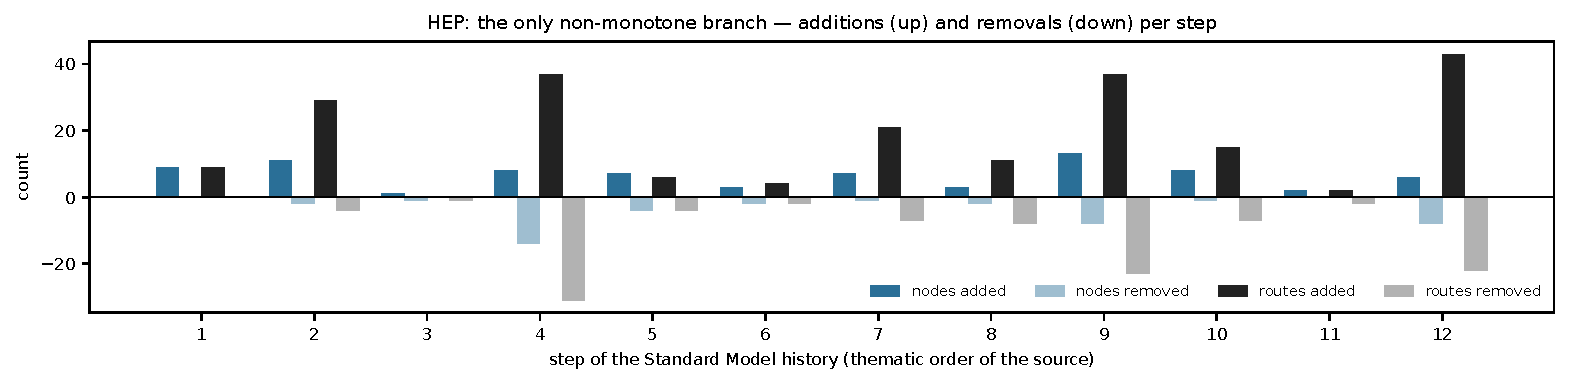
\includegraphics[width=\textwidth]{fig_evo_hep_removals.pdf}
\caption{Nodes and routes added (up) and removed (down) per step of the Standard Model history.}\label{fig:evo_hep_removals}
\end{figure}

\section{Rules on the year axis}\label{sec:rules-time}
Every route of the four branches is attributed to a rule of \cref{ch:rules}: in the reader, R11 (derive) or R12 (fail); in the history, by its kind (\id{enters} $\to$ R4, \id{predicts}/\id{frames}/\id{candidate} $\to$ R2, \id{calibrates} $\to$ R9, \id{backedge} $\to$ R1/R3, \id{lineage} $\to$ R7/R10, \id{subset} $\to$ the observable-family coarse-graining); in the effect networks, R14 (closure) split by the polarity of the closing route, and R13 (open cell) for routes of open status. \Cref{tab:evo_rules_decade} counts the firings per decade and \cref{fig:evo_hep_rules} places the automatically detected rule firings of the Standard Model replay (\cref{sec:detection}) on the year axis.

The connection between the rules and the node and edge numbers is the identity of \cref{thm:identity} read rule by rule. With $\Delta V(T)$ the arrivals of year $T$ and $\Delta E(T)=\Delta E_{\mathrm{arr}}(T)+\Delta E_{\mathrm{clo}}(T)$ the arrival and closure routes:
\begin{itemize}[nosep]
\item R11 (derive) adds one route and $0$ to $k$ nodes; in the reader it contributes \EEMSumArrDeg{} arrival incidences over \EEMVfin{} nodes and only \EEMClosures{} closures, so $\Delta E_{\mathrm{arr}}$ carries the reader. R12 (fail) adds one no-go route with the same counts.
\item R4 (route) and R1/R3 (partition--extend) in the history add routes with their nodes ($\Delta V>0$, $\Delta E_{\mathrm{arr}}>0$); R2 (a model node for a flagged observable) adds a node and its routes; R9 (calibrate) adds a route between a model and an observable, dated in the data with the observable it calibrates and therefore an arrival route; the history's \EHEPClosures{} closures are the entry and back-edge routes of the electron and proton sectors into unitary evolution at the Fock-space step, dated one year after their endpoints; R7/R10 (absorb, cluster) remove: they are the negative terms of the history's curve.
\item R13 (open cell) adds no route and no node: it is the term of the agenda, not of $E$; its firings are the open-status routes the data record (\EgptCensusOpenFinal{} open cells remain in GPT at 2026 under the designated pairs). R14 (close) adds one route and no node in \EGPTClosures{} of \EGPTEfin{} GPT routes and \EQRTClosures{} of \EQRTEfin{} QRT routes; it is the closure term.
\end{itemize}
Hence $\Delta V$ is driven by R2, R4, R1/R3 and the arrivals of R11; $\Delta E_{\mathrm{clo}}$ by R14 (and, rarely, by R4/R1 routes dated after their endpoints and by the reader's late derivations); and the only negative deltas are R7/R10. The densification exponent summarises the balance: $\alpha>1$ in every branch because closures and multi-route arrivals add routes without nodes.

\begin{figure}[htbp]\centering
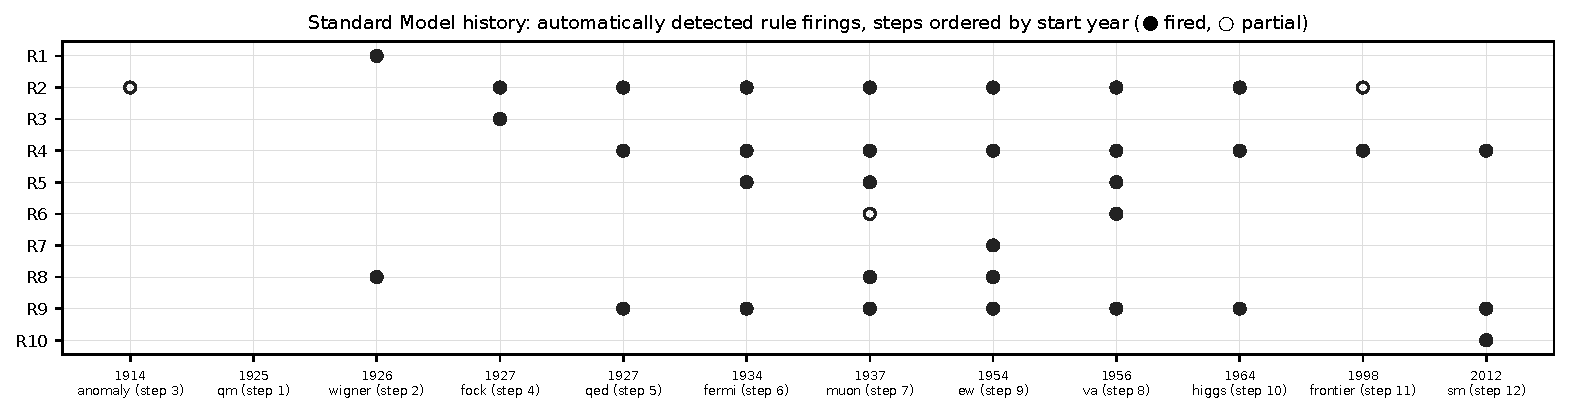
\includegraphics[width=\textwidth]{fig_evo_hep_rules.pdf}
\caption{Rule firings of the Standard Model history detected from structure (\cref{sec:detection}), with the steps ordered by their start year.}\label{fig:evo_hep_rules}
\end{figure}

\section{Temporal rules}\label{sec:te}
The following regularities are read off the dated data in the same spirit as R1--R10 were read off one history: they are stated so that a new branch can violate them.
\begin{description}[nosep]
\item[TE1 (arrival).] A node enters with its arrival routes, dated the same year; the mean degree at arrival is branch-specific (EM \EEMMeanArrDeg{}, HEP \EHEPMeanArrDeg{}, GPT \EGPTMeanArrDeg{}, QRT \EQRTMeanArrDeg{}) and is the dominant term of $E$ in the reader and the history.
\item[TE2 (closure).] In the effect networks a large share of routes are closures (GPT \EGPTClosureFrac\%, QRT \EQRTClosureFrac\%) with median latency \EGPTLatMedian{} and \EQRTLatMedian{} years: the census (R13) is worked off years after the nodes appear.
\item[TE3 (preferential closure).] Closures attach to nodes of above-average degree (ratios \EGPTPAratio{}, \EQRTPAratio{}, \EEMPAratio{}).
\item[TE4 (densification).] $E\propto V^{\alpha}$ with $1<\alpha<2$ in every branch (\EEMAlpha{}, \EHEPAlpha{}, \EGPTAlpha{}, \EQRTAlpha{}).
\item[TE5 (removal).] Only the history removes, by absorption into a successor or by the final clustering; the reader and the effect networks are monotone.
\item[TE6 (transfer).] A shared concept appears in a second branch with a lag (median \ElagMedian{} years); between the effect networks the dominant direction is effect network $\to$ resource network (\EfirstGPTamongGQ{} to \EfirstQRTamongGQ{}, \EtieGQ{} ties).
\end{description}

%=====================================================================
\chapter{The method in the evolution}\label{ch:method-time}

\section{Phases}
Part I named the loop observe $\to$ hypothesise $\to$ feed back $\to$ observe and wrote it as \cref{alg:step}. On the year axis each event of the four branches is assigned a \emph{phase} mechanically, by its layer (for a node) or its kind and status (for a route), as in \cref{tab:phase_map}. The assignment is the only hand-made element of this part, and it is a lookup table: no event is placed by reading its content.
\begin{table}[htbp]\centering\small
\caption{Phase assignment of events. A node arrival is assigned by its layer; a route by its universal kind, with open status overriding to \emph{deficit}.}\label{tab:phase_map}
\begin{tabular}{@{}lp{10.5cm}@{}}\toprule
Phase & Events \\\midrule
observe & O-node arrival; \id{witness}, \id{pairs} routes \\
deficit & routes of open status (R13 open cells) \\
hypothesize & M-node arrival; \id{frames}, \id{candidate}, \id{generates} \\
restructure & S-node arrival; \id{enters}, \id{backedge}, \id{member}, \id{satisfies} \\
predict & \id{derives}, \id{predicts}, \id{implies}, \id{necessary}, \id{enables}, \id{converts\_to}, \id{activates}, \id{reversible}, \id{hosts}, \id{bounds} \\
falsify & \id{failed}, \id{not\_implies}, \id{forbids}, \id{hides}, \id{excludes}, \id{distinct}, \id{violates}, \id{irreversible} \\
calibrate & \id{calibrates} \\
reduce & \id{lineage}, \id{subset}, \id{equiv}, \id{specializes}, \id{contains} \\
\bottomrule\end{tabular}
\end{table}

\Cref{tab:evo_merged_phases} and \cref{fig:evo_phases} count the \EphaseTotal{} events of the evolutionary network (\EmergedV{} arrivals and \EmergedE{} routes) by phase and decade: observe \Ephaseobserve{}, deficit \Ephasedeficit{}, hypothesize \Ephasehypothesize{}, restructure \Ephaserestructure{}, predict \Ephasepredict{}, falsify \Ephasefalsify{}, calibrate \Ephasecalibrate{}, reduce \Ephasereduce{}. Three readings of the table are supported by the counts.
\begin{enumerate}[nosep]
\item \emph{The phases run concurrently.} From the 1820s on, every decade with ten or more events (\EnBigDecades{} decades) contains at least \EminActivePhases{} phases, and the \EdecadesAllPhases{} contain all eight. The loop is not a sequence of eras; it is a cycle executed many times in parallel on different parts of the graph, which is what \cref{alg:step} does when it is run per event.
\item \emph{The branch types have phase profiles} (right panel of \cref{fig:evo_phases}). The reader is predict-heavy (derivations), the history restructure-heavy (sectors entering models, back-edges), the nonclassicality network falsify- and predict-heavy (theorems of both polarities), the resource-theory network observe- and hypothesize-heavy (witnesses and resource definitions). The profile is a consequence of the layer-pair signature of \cref{ch:types}: a type-D signature produces derivations, a type-H signature produces entries, a type-E signature produces closures.
\item \emph{Falsification is late and branch-specific.} The first falsify route of the reader is dated \EEMFirstFalsify{} (the classical derivations that fail at the quantum boundary), of the nonclassicality network \EGPTFirstFalsify{}, of the resource-theory network \EQRTFirstFalsify{} (its first no-go route, Werner's local model for entangled states, is a membership route dated 1989 and counts as restructure); the history has no falsify route, because in the data its refutations are recorded as removals and replacements (R7/R10, \cref{sec:removals}), not as routes. The decade with the most falsify events is the \EdecadeMaxfalsify{}s (\EdecadeMaxfalsifyN{}), the decade with the most restructure events the \EdecadeMaxrestructure{}s (\EdecadeMaxrestructureN{}, the building of the Fock-space and sector structure of the history).
\end{enumerate}
\begin{table}[htbp]\centering\small
\caption{Events of the evolutionary network by phase and decade.}\label{tab:evo_merged_phases}
\resizebox{0.95\textwidth}{!}{\begin{tabular}{@{}lrrrrrrrrr@{}}\toprule
Decade & observe & deficit & hypothesize & restructure & predict & falsify & calibrate & reduce & total \\\midrule
1680s & 3 & 0 & 2 & 1 & 3 & 0 & 0 & 0 & 9 \\
1740s & 1 & 0 & 1 & 0 & 0 & 0 & 0 & 0 & 2 \\
1770s & 0 & 0 & 1 & 0 & 0 & 0 & 0 & 0 & 1 \\
1780s & 0 & 0 & 2 & 1 & 2 & 0 & 0 & 0 & 5 \\
1790s & 2 & 0 & 0 & 0 & 0 & 0 & 0 & 0 & 2 \\
1810s & 0 & 0 & 1 & 1 & 2 & 0 & 0 & 0 & 4 \\
1820s & 6 & 0 & 9 & 5 & 19 & 0 & 0 & 0 & 39 \\
1830s & 2 & 0 & 1 & 0 & 2 & 0 & 0 & 0 & 5 \\
1840s & 2 & 0 & 1 & 1 & 6 & 0 & 0 & 0 & 10 \\
1850s & 0 & 0 & 2 & 0 & 2 & 0 & 0 & 0 & 4 \\
1860s & 0 & 0 & 0 & 1 & 3 & 0 & 0 & 0 & 4 \\
1870s & 1 & 0 & 4 & 1 & 8 & 0 & 0 & 0 & 14 \\
1880s & 2 & 0 & 3 & 1 & 3 & 0 & 0 & 0 & 9 \\
1890s & 1 & 0 & 3 & 1 & 5 & 0 & 0 & 0 & 10 \\
1900s & 7 & 0 & 3 & 3 & 14 & 2 & 0 & 0 & 29 \\
1910s & 6 & 0 & 2 & 2 & 4 & 1 & 0 & 0 & 15 \\
1920s & 10 & 0 & 18 & 25 & 14 & 0 & 1 & 3 & 71 \\
1930s & 13 & 0 & 6 & 57 & 10 & 0 & 1 & 3 & 90 \\
1940s & 7 & 0 & 7 & 2 & 13 & 3 & 1 & 1 & 34 \\
1950s & 5 & 0 & 8 & 2 & 23 & 0 & 1 & 4 & 43 \\
1960s & 6 & 0 & 9 & 31 & 11 & 0 & 5 & 10 & 72 \\
1970s & 4 & 0 & 5 & 1 & 2 & 1 & 1 & 2 & 16 \\
1980s & 12 & 0 & 5 & 28 & 11 & 4 & 0 & 0 & 60 \\
1990s & 16 & 1 & 14 & 2 & 12 & 5 & 0 & 2 & 52 \\
2000s & 16 & 1 & 16 & 20 & 19 & 12 & 0 & 5 & 89 \\
2010s & 47 & 7 & 55 & 38 & 35 & 27 & 2 & 24 & 235 \\
2020s & 12 & 1 & 6 & 10 & 16 & 9 & 0 & 6 & 60 \\
\midrule total & 181 & 10 & 184 & 234 & 239 & 64 & 12 & 60 & 984 \\
\bottomrule\end{tabular}
}
\end{table}
\begin{figure}[htbp]\centering
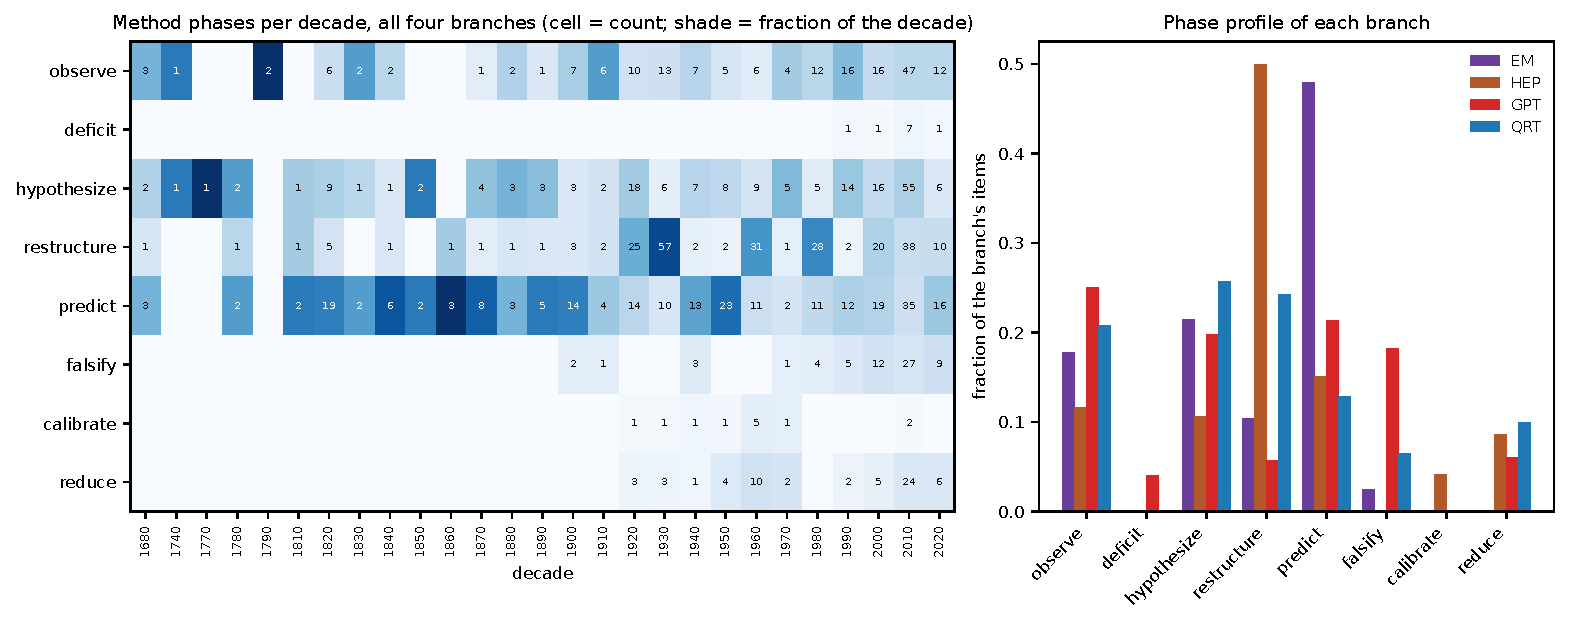
\includegraphics[width=\textwidth]{fig_evo_phases.pdf}
\caption{Left: events per decade by phase, all four branches (cell = count, shade = fraction of the decade). Right: phase profile of each branch.}\label{fig:evo_phases}
\end{figure}

\section{The philosophical structure, as graph operations}\label{sec:philosophy}
The phases are the operational form of positions in the philosophy of science. The correspondence below is stated with the data as evidence, and it records where the data do not support the received picture.
\begin{description}
\item[Falsification \citep{popper1959}.] A no-go or failed route. The reader's \EemFailedTotal{} failed derivations (R12) are falsifications of classical derivations by quantum observables, each resolved by a later route; in the nonclassicality network the first incident route of \EgptMnoGoFirst{} of \EgptMtotal{} model nodes is a pure no-go (\EgptMnoGoAny{} include one): a subtheory is introduced by what it cannot produce. In the history the anomaly steps (an observable with no model route, R2's precondition) are the falsifying events, and the data record their resolution as removal and replacement rather than as a route.
\item[Research programmes \citep{lakatos1970}.] A hard core that survives and a protective belt that is replaced. The data show the belt: all \EhepMfundAll{} fundamental model nodes, the \EhepMeffAll{} effective and the \EhepMcandAll{} candidate model of the history are removed, by absorption into successors and finally into the Lagrangian clusters; the \EhepMclusterAll{} cluster nodes and \EhepMframeKept{} of the \EhepMframeAll{} frames persist; the effect networks never remove their \EgptAxioms{} (GPT) and \EqrtAxioms{} (QRT) axiom nodes. The data do not show a protected core of \emph{model content} in the history: every model node that is not a frame or a cluster is replaced. What persists is structural (the frames that survive: unitary evolution, the observable postulate, the quantum field on Fock space; the particle Lagrangian is the one frame removed) and the end product (the clusters). The thesis records this as a finding about the data, not as a refutation of the reading, since absorption with a lineage edge (reduce) is different from refutation (falsify), and the engine distinguishes the two.
\item[Paradigm change \citep{kuhn1962}.] Restructuring of the state layer. In the graph a revolution is a sequence of ordinary operations (\cref{ch:limits}); on the year axis the restructure phase peaks in the \EdecadeMaxrestructure{}s with \EdecadeMaxrestructureN{} events, the re-partition of the one-particle Hilbert space into Fock space and sectors (R1/R3, back-edges). What the data do not show is incommensurability: the glue identifications across every restructuring (\EmergedGlue{} at 2026, growing through the 1920s--1930s) are concepts that keep their identity in the reader and the history while their layer and routes change.
\item[Holism \citep{duhem1954,quine1951}.] AND routes. \EemDeriveAND{} of \EemDeriveTotal{} derivations and \EemFailedAND{} of \EemFailedTotal{} failed routes of the reader have two or more inputs (model and state jointly); \EhepEntersAND{} of \EhepEntersTotal{} state$\to$model routes of the history are AND routes with occupation numbers. A failed AND route cannot by itself locate the faulty input, and the reader's resolutions (\cref{ch:readers}) are indeed new routes rather than deletions of one input.
\item[Explanation \citep{hempel1948}.] An M$\to$O route into an effect. The explanation lag of \cref{sec:arrivals} measures the years between an effect's appearance and its first model route: \EgptEffectsWithM{} of \EgptEffects{} effects have one, mean lag \EgptLagMean{} years, \EgptLagZero{} explained in their first year, Bell nonlocality after \EgptLagBell{} years. In the history every prediction is a single M$\to$O route (\EhepPredictsMO{} of \EhepPredictsTotal{}), the deductive-nomological form with the state dependence carried by the preceding \id{enters} routes.
\item[Discovery and justification \citep{reichenbach1938}; reduction \citep{nagel1961}.] The year of a route is its context of discovery (when its ingredients were in print), its status and polarity its justification; reduce routes (\id{lineage}, \id{subset}, \id{equiv}, \id{specializes}, \id{contains}; \Ephasereduce{} events) are the inter-theoretic reductions, and in the history they are the operations that make a model node removable: each of the \EhepRemovedModel{} removed model nodes (\EhepRemovedModelWithReduce{} of \EhepRemovedModel{}) is the source of a lineage or cluster-membership route (\EhepReduceRoutes{} such routes) naming its successor.
\end{description}

\section{The loop in time}
The eight phases, in the order of \cref{alg:step}, are observe $\to$ deficit $\to$ hypothesize $\to$ restructure $\to$ predict $\to$ falsify $\to$ calibrate $\to$ reduce. The evolutionary network shows the loop at three scales. At the scale of a decade all phases co-occur (\cref{tab:evo_merged_phases}). At the scale of a branch the profile is fixed by the signature. At the scale of a single node the order is visible as latencies: a witness and its effect appear together (observe), the effect's model route arrives \EgptLagMean{} years later on average (predict/explain), closures with the rest of the network follow with median latency \EGPTLatMedian{} years (TE2), and, in the history, a model node is reduced into its successor at a later step (TE5). The methodology written as an algorithm in \cref{ch:algorithm} is therefore also a description of the time series: \cref{alg:step} run once per event, with the solver's latency as the only quantity the engine does not compute.


%=====================================================================
\part{Closing}\label{part:closing}
\chapter{Discussion and limitations}\label{ch:limits}
\begin{itemize}
\item \textbf{Gaps are curation-relative.} An uncharted cell or an empty sector--term cell means that the compiled data record no edge, not that none exists. The project's standing rule is that a relation the literature establishes must already be an edge, so a gap is a question the compilation does not answer; closing it may be a literature fill. The engine cannot tell a forbidden cell from an omitted one; that is content.
\item \textbf{Page view versus state of knowledge.} The Standard Model page draws selections; the engine's cumulative view is a reconstruction with explicit rules (persistence of observables, successor map, family closure). Different rules give different final deficits (one with family closure, four without), and the thesis states which rule it uses.
\item \textbf{The gluing is curated.} The \NnConcepts{} identifications were made by reading labels and descriptions; they are listed with justifications so that each can be disputed by naming the concept. Several are identifications at a level of detail (the Compton shift and the Compton cross section; the Clifford group and the stabilizer operations; the general-group and the $U(1)$ symmetric states) and are marked as such.
\item \textbf{Sub-layers of the readers are heuristic.} The point/field/Hilbert sorting of reader states is by era and label words; it does not affect any count in the thesis and is recorded for the reader of the data.
\item \textbf{Scope of the instances.} The Standard Model branch omits the strong sector, the electromagnetism reader stops at QED, the textbook reader is one book, and the quantum networks are reviews, not exhaustive compilations. The grand network inherits these scopes.
\item \textbf{The calendar axis is an ingredient chronology.} A route of the quantum networks is dated by the oldest source it cites (\cref{sec:dating}); this is a lower bound on the year the route was established and can precede the historical origin of a concept or follow it (\cref{sec:dating-caveat}). The project-dated nodes are flagged and excluded from the lags; the growth quantities are recomputed under the latest-source convention (\cref{tab:evo_robust}) and the conclusions of Part II are those that survive the change. No statement of Part II is a claim about the history of physics beyond the sources the networks cite.
\item \textbf{The history's steps are thematic.} The Standard Model page orders its steps by theme (the anomaly step starts in 1914, the Wigner step in 1926); the year index uses the nodes' own year fields and places a removal at the start year of the removing step, never before the item's own year, and the final view at 2012. Items added and removed by steps whose ranges overlap are present for one year on the axis.
\item \textbf{The phase table is hand-made.} The assignment of kinds to phases (\cref{tab:phase_map}) is the one lookup table of Part II that is not computed; it is stated in full so that a different assignment can be run. The philosophical correspondences of \cref{sec:philosophy} are readings of the counts, and the thesis records where the counts do not fit the received picture rather than adjusting either.
\item \textbf{The rules are regularities, not laws.} R1--R10 were read off one history and are written so that they can fail on the next instance; they describe the normal growth of a research programme in Lakatos's sense \citep{lakatos1970} rather than the revolutions of Kuhn's \citep{kuhn1962}, and the replay suggests why: in the graph a revolution is a sequence of ordinary operations (partition, extend, merge, absorb) whose count deltas are the same as those of normal growth; the replay shows they are decidable from structure in 117 of 120 cells on that history and locates the cell that is not.
\end{itemize}

%=====================================================================
\chapter{Conclusion}
The six instances of the Great Epistemic Network are one object. Normalised into a single schema they differ in how they sort the three layers, and the difference is captured by one matrix per branch, the layer-pair signature; the three supports it takes define the dynamic, historical and effect branches, and the contraction lemma relates the last two. Their changes decompose into two dozen primitive operations whose count deltas are stated, and the rules that fire the operations are predicates that an engine evaluates: on the Standard Model history the engine recovers the hand-assigned rules from structure alone with three explained exceptions; on the readers it verifies the filtration and resolves the failed routes; on the quantum networks it reproduces the census that is their research agenda and applies the same census to the other branches. The research agenda of any concept graph, which is where the next model node, the next theorem or the next paragraph must go, is computable in linear time. What the agenda does not contain is the content that fills it, and the thesis names the solvers that supply it. The grand network, with its \NnNodes{} nodes, \NnRoutes{} routes and \NnConcepts{} shared concepts, is delivered as data so that the next branch, the strong sector or a second textbook, can be added by the same loop.

Placed on a calendar axis, four of the branches show how the loop runs in time. The effect and resource networks grow by arrivals and, to a large degree, by closures with latencies of years; the reader and the history grow by arrivals; only the history removes. The counts obey an exact arrival--closure identity, densify with exponents between one and two, close preferentially around the best-connected nodes, and transfer concepts between branches with lags of a decade; the rules of Part I account for every route and for the sign of every change in the counts. The method phases run concurrently in every decade, their mix fixed by the branch's signature, and the philosophical positions on how science grows appear as graph operations whose frequencies can be counted, with the data agreeing with some readings and not with others. The evolutionary network of \EmergedV{} nodes and \EmergedE{} routes is delivered with a year slider so that each of these statements can be watched happening.

%=====================================================================
\chapter{AI-generation disclosure}\label{ch:ai}
This thesis, the engine (\texttt{gen\_engine}), the build scripts (\texttt{build.py}, \texttt{build\_evolution.py}), the gluing table, the chronology rules, the phase table, the figures, the tables and the two explorer pages were generated by Claude (Anthropic) in working sessions directed by the author, from the released data files of the six repositories cloned at the commits listed in \cref{sec:provenance}. The author takes responsibility for the content and invites correction: every count can be recomputed with \texttt{python3 build.py}, every identification in \cref{app:concepts} can be disputed by concept id, and every rule predicate is stated in \cref{sec:detection}. The six instances themselves were produced earlier in the same project, also with AI assistance, and are cited as their repositories.

\appendix
%=====================================================================
\chapter{The gluing catalogue}\label{app:concepts}
\scriptsize
\begin{longtable}{@{}p{3.1cm}p{3.6cm}p{5.0cm}p{2.9cm}@{}}\toprule
Concept & Label & Members (branch: native ids) & Roles \\\midrule\endhead
\texttt{force} & Force (on a body / on a charge) & EM: F; UP: F & EM=O, UP=O \\
\texttt{position} & Position & EM: r; UP: r; HEP: o\_x & EM=O, UP=O, HEP=O \\
\texttt{velocity} & Velocity & EM: v; UP: v & EM=O, UP=O \\
\texttt{momentum} & Momentum & UP: p; HEP: o\_p & UP=O, HEP=O \\
\texttt{mass} & Mass & UP: m; HEP: o\_m & UP=O, HEP=O \\
\texttt{time\_\allowbreak{{}}derivative} & Time derivative & EM: ddt; UP: ddt & EM=M, UP=M \\
\texttt{vector\_\allowbreak{{}}addition} & Vector addition & EM: vec; UP: vadd & EM=M, UP=M \\
\texttt{cross\_\allowbreak{{}}product} & Cross (vector) product & EM: cross; UP: cross & EM=M, UP=M \\
\texttt{electric\_\allowbreak{{}}charge} & Electric charge & EM: q; UP: q & EM=O, UP=O \\
\texttt{charge\_\allowbreak{{}}conservation} & Conservation of charge & EM: addq; UP: qcons & EM=M, UP=M \\
\texttt{coulomb\_\allowbreak{{}}law} & Coulomb's law & EM: coul; UP: coul & EM=M, UP=M \\
\texttt{point\_\allowbreak{{}}charges} & Point-charge configuration & EM: pts; UP: pts & EM=S, UP=S \\
\texttt{superposition} & Superposition of sources & EM: sup; UP: esup & EM=M, UP=M \\
\texttt{charge\_\allowbreak{{}}density} & Continuous charge distribution & EM: rho; UP: chdist & EM=S, UP=S \\
\texttt{electric\_\allowbreak{{}}field} & Electric field (state) & EM: Efield; UP: Efield & EM=S, UP=S \\
\texttt{electric\_\allowbreak{{}}flux} & Electric flux & EM: PhiE; UP: PhiE & EM=O, UP=O \\
\texttt{electrostatic\_\allowbreak{{}}energy} & Electrostatic (electric potential) energy & EM: U; UP: Ue & EM=O, UP=O \\
\texttt{electric\_\allowbreak{{}}potential} & Electric potential (state) & EM: phi; UP: Vfield & EM=S, UP=S \\
\texttt{capacitance} & Capacitance & EM: C; UP: Cap & EM=O, UP=O \\
\texttt{current} & Electric current & EM: I; UP: curr & EM=O, UP=O \\
\texttt{current\_\allowbreak{{}}density} & Current density (state) & EM: J; UP: Jcur & EM=S, UP=S \\
\texttt{resistance} & Resistance & EM: R; UP: Rres & EM=O, UP=O \\
\texttt{ohm\_\allowbreak{{}}law} & Ohm's law & EM: ohm; UP: ohm & EM=M, UP=M \\
\texttt{magnetic\_\allowbreak{{}}field} & Magnetic field (state) & EM: Bfield; UP: Bfield & EM=S, UP=S \\
\texttt{magnetic\_\allowbreak{{}}field\_\allowbreak{{}}value} & Magnetic field value & EM: B; UP: Bval & EM=O, UP=O \\
\texttt{biot\_\allowbreak{{}}savart} & Biot-Savart law & EM: bs; UP: bs & EM=M, UP=M \\
\texttt{emf} & Electromotive force & EM: emf; UP: emf & EM=O, UP=O \\
\texttt{magnetic\_\allowbreak{{}}flux} & Magnetic flux & EM: PhiB; UP: PhiB & EM=O, UP=O \\
\texttt{faraday\_\allowbreak{{}}law} & Faraday's law & EM: faraday; UP: faraday; LG: Fa & EM=M, UP=M, LG=M \\
\texttt{maxwell\_\allowbreak{{}}equations} & Maxwell's equations & EM: maxwell; UP: maxwell & EM=M, UP=M \\
\texttt{em\_\allowbreak{{}}field\_\allowbreak{{}}state} & Electromagnetic field state (E, B) & EM: EB; UP: EB; LG: x & EM=S, UP=S, LG=S \\
\texttt{speed\_\allowbreak{{}}of\_\allowbreak{{}}light} & Speed of light & EM: c; UP: c & EM=O, UP=O \\
\texttt{electric\_\allowbreak{{}}energy\_\allowbreak{{}}density} & Electric energy (density) & UP: uE; LG: uE & UP=O, LG=O \\
\texttt{magnetic\_\allowbreak{{}}energy\_\allowbreak{{}}density} & Magnetic energy (density) & UP: uB; LG: uB & UP=O, LG=O \\
\texttt{poynting\_\allowbreak{{}}vector} & Poynting vector & EM: S; UP: Spoynt & EM=O, UP=O \\
\texttt{poynting\_\allowbreak{{}}theorem} & Poynting's theorem (energy bookkeeping) & EM: poynt; LG: fJE, fPi, fSin, fSout & EM=M, LG=M \\
\texttt{lorentz\_\allowbreak{{}}transformation} & Lorentz transformation / group & EM: lorentz; UP: lorentzT & EM=M, UP=M \\
\texttt{poisson\_\allowbreak{{}}structure} & Poisson bracket / symplectic structure & EM: pb; GPT: ax-symplectic & EM=M, GPT=M \\
\texttt{poisson\_\allowbreak{{}}to\_\allowbreak{{}}commutator} & Canonical commutator / Poisson-to-commutator lift & EM: comm; GPT: ax-moyal & EM=M, GPT=M \\
\texttt{planck\_\allowbreak{{}}constant}$\ast$ & Planck's constant & EM: hbar; UP: hbar; GPT: ax-hbar & EM=O, UP=O, GPT=M \\
\texttt{blackbody}$\ast$ & Blackbody radiation / spectrum & EM: bbspec; UP: bbrad & EM=O, UP=S \\
\texttt{planck\_\allowbreak{{}}relation} & Planck's relation / hypothesis & EM: planck; UP: planck & EM=M, UP=M \\
\texttt{photon}$\ast$ & Photon & EM: photon; UP: photon; HEP: s\_g & EM=O, UP=S, HEP=S \\
\texttt{spectral\_\allowbreak{{}}lines} & Spectral lines (hydrogen) & EM: spectra; UP: Hspec & EM=O, UP=O \\
\texttt{bohr\_\allowbreak{{}}model}$\ast$ & Bohr model / orbits & EM: bohr; UP: bohr & EM=S, UP=M \\
\texttt{hydrogen\_\allowbreak{{}}levels}$\ast$ & Hydrogen energy levels & UP: bohrlev; HEP: o\_E & UP=S, HEP=O \\
\texttt{schrodinger\_\allowbreak{{}}evolution} & Schrodinger equation / unitary evolution & EM: schro; UP: tdse; HEP: m\_U; GPT: p-unitary & EM=M, UP=M, HEP=M, GPT=M \\
\texttt{hilbert\_\allowbreak{{}}state} & Hilbert-space state / wave function & EM: hilb; UP: psi; HEP: H1 & EM=S, UP=S, HEP=S \\
\texttt{observable\_\allowbreak{{}}postulate} & Operator algebra and Born rule & EM: born, ops; HEP: m\_A & EM=M, HEP=M \\
\texttt{outcome\_\allowbreak{{}}statistics} & Outcome statistics / expectation values & EM: expect; UP: expval & EM=O, UP=O \\
\texttt{lagrangian} & Lagrangian / action principle & EM: action; HEP: m\_L & EM=M, HEP=M \\
\texttt{creation\_\allowbreak{{}}annihilation} & Creation and annihilation operators / quantum field & EM: ladder; HEP: m\_field & EM=M, HEP=M \\
\texttt{electron\_\allowbreak{{}}field} & Electron-positron field / electron sector & EM: psiop; HEP: s\_e & EM=S, HEP=S \\
\texttt{qed\_\allowbreak{{}}interaction} & QED interaction (Lagrangian / vertex) & EM: qedL; HEP: m\_qed & EM=M, HEP=M \\
\texttt{cross\_\allowbreak{{}}section} & Cross sections & EM: xsec; HEP: o\_sig & EM=O, HEP=O \\
\texttt{lamb\_\allowbreak{{}}shift} & Lamb shift & EM: lamb; HEP: o\_lamb & EM=O, HEP=O \\
\texttt{anomalous\_\allowbreak{{}}moment} & Anomalous magnetic moment of the electron & EM: amm; HEP: o\_ae & EM=O, HEP=O \\
\texttt{fine\_\allowbreak{{}}structure\_\allowbreak{{}}constant} & Fine-structure constant & EM: alpha; HEP: o\_alpha & EM=O, HEP=O \\
\texttt{compton} & Compton effect & UP: compton; HEP: o\_compton & UP=O, HEP=O \\
\texttt{electron\_\allowbreak{{}}spin} & Electron spin & UP: spin; HEP: o\_S & UP=O, HEP=O \\
\texttt{orbital\_\allowbreak{{}}angular\_\allowbreak{{}}momentum} & Quantized orbital angular momentum & UP: Lq; HEP: o\_L & UP=O, HEP=O \\
\texttt{particle\_\allowbreak{{}}decay}$\ast$ & Particle production and decay & UP: decay; HEP: o\_prod & UP=S, HEP=O \\
\texttt{standard\_\allowbreak{{}}model} & The Standard Model Lagrangian & UP: sm; HEP: c\_gf, c\_gg, c\_hg, c\_pot, c\_yuk & UP=M, HEP=M \\
\texttt{gibbs\_\allowbreak{{}}state} & Gibbs (thermal) state & UP: mbd; GPT: s-thermal; QRT: d-gibbs, sF-ath & UP=S, GPT=S, QRT=S \\
\texttt{second\_\allowbreak{{}}law}$\ast$ & Second law(s) of thermodynamics & UP: slaw; GPT: t-secondlaws; QRT: wQ-ath & UP=M, GPT=O, QRT=O \\
\texttt{interference}$\ast$ & Two-path (second-order) interference & UP: dslit; GPT: e-interf2 & UP=S, GPT=O \\
\texttt{entangled\_\allowbreak{{}}states} & Entangled states & GPT: s-ent; QRT: sR-ent & GPT=S, QRT=S \\
\texttt{separable\_\allowbreak{{}}states} & Separable states & GPT: s-sep; QRT: sF-ent & GPT=S, QRT=S \\
\texttt{bound\_\allowbreak{{}}entangled} & Bound (PPT) entangled states & GPT: s-bound; QRT: d-bound & GPT=S, QRT=S \\
\texttt{magic\_\allowbreak{{}}states} & Magic (non-stabilizer) states & GPT: s-magic; QRT: sR-mag & GPT=S, QRT=S \\
\texttt{stabilizer\_\allowbreak{{}}states} & Stabilizer states & GPT: s-stab; QRT: sF-mag & GPT=S, QRT=S \\
\texttt{coherent\_\allowbreak{{}}states} & Basis-coherent states & GPT: s-coh; QRT: sR-coh & GPT=S, QRT=S \\
\texttt{athermal\_\allowbreak{{}}states} & Athermal states & GPT: s-athermal; QRT: sR-ath & GPT=S, QRT=S \\
\texttt{wigner\_\allowbreak{{}}negative} & Wigner-negative states & GPT: s-wneg; QRT: sR-nga & GPT=S, QRT=S \\
\texttt{discordant\_\allowbreak{{}}states} & Discordant states & GPT: s-discord; QRT: sR-dis & GPT=S, QRT=S \\
\texttt{zero\_\allowbreak{{}}discord} & Classical-classical (zero-discord) states & GPT: s-zerodisc; QRT: sF-dis & GPT=S, QRT=S \\
\texttt{symmetric\_\allowbreak{{}}states} & Symmetric (TTS / energy-diagonal) states & GPT: s-tts; QRT: sF-asy & GPT=S, QRT=S \\
\texttt{asymmetric\_\allowbreak{{}}states} & Asymmetric (energy-coherent) states & GPT: s-cohE; QRT: sR-asy & GPT=S, QRT=S \\
\texttt{locc} & LOCC / non-entangling operations & GPT: p-locc; QRT: pF-ent & GPT=M, QRT=M \\
\texttt{thermal\_\allowbreak{{}}operations} & Thermal operations & GPT: p-thermalops; QRT: pF-ath & GPT=M, QRT=M \\
\texttt{covariant\_\allowbreak{{}}operations} & Covariant (symmetric) operations & GPT: p-cov; QRT: pF-asy & GPT=M, QRT=M \\
\texttt{incoherent\_\allowbreak{{}}operations} & Incoherent operations & GPT: p-incoh; QRT: pF-coh & GPT=M, QRT=M \\
\texttt{stabilizer\_\allowbreak{{}}operations} & Stabilizer / Clifford operations & GPT: p-clifford; QRT: pF-mag & GPT=M, QRT=M \\
\texttt{gaussian\_\allowbreak{{}}operations} & Gaussian operations / protocols & GPT: p-gaussU; QRT: pF-nga & GPT=M, QRT=M \\
\texttt{stabilizer\_\allowbreak{{}}subtheory} & Stabilizer subtheory & GPT: m-stab-even, m-stab-odd; QRT: m-mag & GPT=M, QRT=M \\
\texttt{gaussian\_\allowbreak{{}}subtheory} & Gaussian subtheory (CV) & GPT: m-gaussian; QRT: m-nga & GPT=M, QRT=M \\
\texttt{bell\_\allowbreak{{}}witness} & Bell / CHSH inequalities & GPT: w-bell; QRT: wD-nlo & GPT=O, QRT=O \\
\texttt{steering\_\allowbreak{{}}witness} & Steering inequalities / LHS tests & GPT: w-steer; QRT: wD-ste & GPT=O, QRT=O \\
\texttt{entanglement\_\allowbreak{{}}witness} & Entanglement witnesses & GPT: w-entw; QRT: wD-ent & GPT=O, QRT=O \\
\texttt{noncontextuality\_\allowbreak{{}}witness} & Noncontextuality inequalities & GPT: w-ncineq; QRT: wD-ctx & GPT=O, QRT=O \\
\texttt{wigner\_\allowbreak{{}}witness} & Wigner-negativity estimators & GPT: w-wig; QRT: wD-nga & GPT=O, QRT=O \\
\texttt{magic\_\allowbreak{{}}witness} & Magic witnesses & GPT: w-magicw; QRT: wD-mag & GPT=O, QRT=O \\
\texttt{coherence\_\allowbreak{{}}monotones} & Coherence monotones & GPT: w-cohw; QRT: wQ-coh & GPT=O, QRT=O \\
\texttt{discord\_\allowbreak{{}}witness} & Local-broadcasting test & GPT: w-discw; QRT: wD-dis & GPT=O, QRT=O \\
\texttt{incompatibility\_\allowbreak{{}}witness} & Incompatibility witnesses / joint-measurability SDP & GPT: w-incomp; QRT: wD-inc & GPT=O, QRT=O \\
\texttt{bell\_\allowbreak{{}}nonlocality}$\ast$ & Bell nonlocality & GPT: e-bell; QRT: sR-nlo & GPT=O, QRT=S \\
\texttt{epr\_\allowbreak{{}}steering}$\ast$ & EPR steering & GPT: e-steer; QRT: sR-ste & GPT=O, QRT=S \\
\texttt{ks\_\allowbreak{{}}contextuality}$\ast$ & Kochen-Specker contextuality & GPT: e-ks, e-ksdep; QRT: sR-ctx & GPT=O, QRT=S \\
\texttt{measurement\_\allowbreak{{}}incompatibility}$\ast$ & Measurement incompatibility & GPT: e-incomp; QRT: sR-inc & GPT=O, QRT=S \\
\texttt{di\_\allowbreak{{}}tasks}$\ast$ & Device-independent tasks & GPT: t-di; QRT: pU-nlo & GPT=O, QRT=M \\
\texttt{one\_\allowbreak{{}}sided\_\allowbreak{{}}di}$\ast$ & One-sided device-independent tasks & GPT: t-1sdi; QRT: pU-ste & GPT=O, QRT=M \\
\texttt{state\_\allowbreak{{}}injection}$\ast$ & State injection / universal computation & GPT: t-mbqc; QRT: pU-mag & GPT=O, QRT=M \\
\texttt{pom\_\allowbreak{{}}rac}$\ast$ & Parity-oblivious multiplexing / RAC advantage & GPT: t-pom; QRT: pU-ctx & GPT=O, QRT=M \\
\texttt{metrology}$\ast$ & Metrology / clocks & GPT: t-metro; QRT: pU-asy & GPT=O, QRT=M \\
\texttt{discrimination} & Discrimination advantage & GPT: t-disc; QRT: t-discrim & GPT=O, QRT=O \\
\bottomrule\end{longtable}

\normalsize

\chapter{Pair census of the nonclassicality network by layer pair}\label{app:pairs}
\small
\begin{longtable}{@{}llrrr@{}}\toprule
layer & layer & pairs & connected & \% \\\midrule\endhead
axiom & axiom & 91 & 2 & 2.2 \\
axiom & effect & 182 & 6 & 3.3 \\
axiom & model & 154 & 14 & 9.1 \\
axiom & process & 182 & 0 & 0.0 \\
axiom & state & 196 & 3 & 1.5 \\
axiom & task & 140 & 2 & 1.4 \\
axiom & witness & 238 & 0 & 0.0 \\
effect & effect & 78 & 12 & 15.4 \\
effect & model & 143 & 13 & 9.1 \\
effect & process & 169 & 6 & 3.6 \\
effect & state & 182 & 15 & 8.2 \\
effect & task & 130 & 8 & 6.2 \\
effect & witness & 221 & 13 & 5.9 \\
model & model & 55 & 1 & 1.8 \\
model & process & 143 & 0 & 0.0 \\
model & state & 154 & 6 & 3.9 \\
model & task & 110 & 0 & 0.0 \\
model & witness & 187 & 0 & 0.0 \\
process & process & 78 & 2 & 2.6 \\
process & state & 182 & 7 & 3.8 \\
process & task & 130 & 1 & 0.8 \\
process & witness & 221 & 0 & 0.0 \\
state & state & 91 & 13 & 14.3 \\
state & task & 140 & 8 & 5.7 \\
state & witness & 238 & 5 & 2.1 \\
task & task & 45 & 0 & 0.0 \\
task & witness & 170 & 0 & 0.0 \\
witness & witness & 136 & 0 & 0.0 \\
\bottomrule\end{longtable}

\normalsize

\chapter{Shared concepts of the two readers with first-appearance paragraphs}\label{app:order}
\small
\begin{longtable}{@{}lrr@{}}\toprule
Concept & EM paragraph & UP paragraph \\\midrule\endhead
force & 2 & 52 \\
position & 2 & 37 \\
velocity & 2 & 26 \\
time\_derivative & 2 & 26 \\
vector\_addition & 2 & 14 \\
electric\_charge & 5 & 307 \\
charge\_conservation & 5 & 308 \\
coulomb\_law & 7 & 313 \\
point\_charges & 8 & 316 \\
superposition & 8 & 315 \\
charge\_density & 10 & 319 \\
electric\_potential & 11 & 337 \\
electric\_flux & 12 & 326 \\
electric\_field & 13 & 317 \\
electrostatic\_energy & 13 & 335 \\
capacitance & 14 & 349 \\
current & 15 & 362 \\
current\_density & 15 & 365 \\
resistance & 15 & 367 \\
ohm\_law & 15 & 368 \\
cross\_product & 18 & 20 \\
magnetic\_field\_value & 18 & 392 \\
biot\_savart & 18 & 403 \\
magnetic\_field & 19 & 391 \\
emf & 20 & 375 \\
magnetic\_flux & 20 & 414 \\
faraday\_law & 20 & 415 \\
speed\_of\_light & 25 & 177 \\
maxwell\_equations & 27 & 450 \\
em\_field\_state & 28 & 452 \\
poynting\_vector & 33 & 455 \\
lorentz\_transformation & 40 & 512 \\
blackbody & 50 & 520 \\
planck\_constant & 51 & 522 \\
planck\_relation & 51 & 522 \\
photon & 52 & 526 \\
spectral\_lines & 53 & 529 \\
bohr\_model & 53 & 532 \\
schrodinger\_evolution & 56 & 548 \\
hilbert\_state & 56 & 542 \\
outcome\_statistics & 57 & 545 \\
\bottomrule\end{longtable}

\normalsize

\chapter{Per-chapter growth of the textbook reader}\label{app:chapters}
\small
\begin{longtable}{@{}llrrrl@{}}\toprule
Chapter & Title & new nodes & routes & carried in & S/M/O \\\midrule\endhead
1.1 & Units and Measurement & 12 & 8 & 0 & 0/0/0 \\
1.2 & Vectors & 8 & 6 & 0 & 0/0/0 \\
1.3 & Motion Along a Straight Line & 17 & 16 & 3 & 0/1/2 \\
1.4 & Motion in Two and Three Dimensions & 14 & 19 & 12 & 1/6/5 \\
1.5 & Newton's Laws of Motion & 11 & 9 & 8 & 1/4/3 \\
1.6 & Applications of Newton's Laws & 9 & 9 & 11 & 0/4/7 \\
1.7 & Work and Kinetic Energy & 5 & 6 & 10 & 0/4/6 \\
1.8 & Potential Energy and Conservation of Energy & 9 & 10 & 6 & 0/2/4 \\
1.9 & Linear Momentum and Collisions & 10 & 13 & 12 & 1/5/6 \\
1.10 & Fixed-Axis Rotation & 12 & 21 & 21 & 2/6/13 \\
1.11 & Angular Momentum & 5 & 6 & 12 & 1/3/8 \\
1.12 & Static Equilibrium and Elasticity & 11 & 11 & 9 & 1/3/5 \\
1.13 & Gravitation & 19 & 19 & 16 & 1/5/10 \\
1.14 & Fluid Mechanics & 16 & 16 & 10 & 0/2/8 \\
1.15 & Oscillations & 11 & 15 & 17 & 2/3/12 \\
1.16 & Waves & 13 & 17 & 13 & 2/3/8 \\
1.17 & Sound & 7 & 9 & 11 & 2/3/6 \\
2.1 & Temperature and Heat & 14 & 14 & 10 & 2/2/6 \\
2.2 & The Kinetic Theory of Gases & 15 & 16 & 8 & 1/1/6 \\
2.3 & The First Law of Thermodynamics & 8 & 9 & 12 & 3/3/6 \\
2.4 & The Second Law of Thermodynamics & 12 & 15 & 7 & 1/4/2 \\
2.5 & Electric Charges and Fields & 14 & 16 & 7 & 0/4/3 \\
2.6 & Gauss's Law & 4 & 5 & 7 & 2/4/1 \\
2.7 & Electric Potential & 5 & 8 & 11 & 2/6/3 \\
2.8 & Capacitance & 8 & 10 & 10 & 3/2/5 \\
2.9 & Current and Resistance & 9 & 11 & 7 & 1/1/5 \\
2.10 & Direct-Current Circuits & 6 & 6 & 9 & 2/2/5 \\
2.11 & Magnetic Forces and Fields & 8 & 12 & 13 & 1/2/10 \\
2.12 & Sources of Magnetic Fields & 7 & 6 & 8 & 2/4/2 \\
2.13 & Electromagnetic Induction & 7 & 8 & 12 & 3/5/4 \\
2.14 & Inductance & 7 & 10 & 12 & 1/5/6 \\
2.15 & Alternating-Current Circuits & 9 & 10 & 11 & 1/5/5 \\
2.16 & Electromagnetic Waves & 7 & 9 & 17 & 2/6/9 \\
3.1 & The Nature of Light & 10 & 12 & 7 & 2/1/4 \\
3.2 & Geometric Optics and Image Formation & 10 & 10 & 3 & 0/3/0 \\
3.3 & Interference & 5 & 5 & 7 & 2/4/1 \\
3.4 & Diffraction & 7 & 7 & 8 & 5/3/0 \\
3.5 & Relativity & 15 & 20 & 14 & 0/8/6 \\
3.6 & Photons and Matter Waves & 16 & 26 & 26 & 5/7/14 \\
3.7 & Quantum Mechanics & 13 & 15 & 13 & 5/6/2 \\
3.8 & Atomic Structure & 11 & 11 & 12 & 4/3/5 \\
3.9 & Condensed Matter Physics & 10 & 15 & 17 & 6/3/8 \\
3.10 & Nuclear Physics & 10 & 11 & 10 & 4/3/3 \\
3.11 & Particle Physics and Cosmology & 9 & 9 & 15 & 4/7/4 \\
\bottomrule\end{longtable}

\normalsize

\chapter{Yearly event logs of the effect networks}\label{app:events}
\small
\subsection*{Nonclassicality network}
\label{tab:evo_events_gpt}
\begin{longtable}{@{}lrrrp{3.4cm}p{5.6cm}@{}}\toprule
Year & nodes & arr.\ routes & closures & nodes added & routes added \\\midrule\endhead
1932 & 2 & 1 & 0 & \texttt{ax-complex}, \texttt{m-quantum} & \texttt{GN7} \\
1933 & 2 & 1 & 0 & \texttt{w-kd}, \texttt{e-kd} & \texttt{W9} \\
1946 & 2 & 2 & 0 & \texttt{ax-moyal}, \texttt{s-wneg} & \texttt{GN4}, \texttt{GN5} \\
1969 & 2 & 1 & 0 & \texttt{w-bell}, \texttt{e-bell} & \texttt{W1} \\
1974 & 1 & 1 & 0 & \texttt{s-gauss} & \texttt{S6} \\
1977 & 1 & 1 & 0 & \texttt{w-wig} & \texttt{W8} \\
1978 & 2 & 1 & 0 & \texttt{ax-hbar}, \texttt{m-classical} & \texttt{GN10} \\
1980 & 3 & 3 & 0 & \texttt{ax-loctom}, \texttt{m-realqm}, \texttt{e-pr} & \texttt{GN6}, \texttt{E8}, \texttt{F5} \\
1982 & 2 & 2 & 0 & \texttt{p-cov}, \texttt{e-incomp} & \texttt{R2}, \texttt{B7} \\
1988 & 5 & 3 & 0 & \texttt{p-weak}, \texttt{w-weakval}, \texttt{w-vis}, \texttt{e-interf2}, \texttt{e-weak} & \texttt{P9}, \texttt{W10}, \texttt{W16} \\
1989 & 2 & 2 & 0 & \texttt{s-ent}, \texttt{e-ctx} & \texttt{R3}, \texttt{B3} \\
1990 & 4 & 3 & 0 & \texttt{ax-epirestrict}, \texttt{m-stab-even}, \texttt{s-thermal}, \texttt{e-ks} & \texttt{GN3}, \texttt{C6}, \texttt{N2} \\
1991 & 0 & 0 & 2 &  & \texttt{MH1}, \texttt{B2} \\
1994 & 4 & 4 & 1 & \texttt{ax-nosig}, \texttt{ax-sorkin}, \texttt{w-sorkin}, \texttt{e-interf3} & \texttt{R6}, \texttt{E1}, \texttt{E9}, \texttt{W1b}, \texttt{W17} \\
1995 & 1 & 1 & 1 & \texttt{p-filter} & \texttt{B5}, \texttt{P7} \\
1996 & 4 & 3 & 0 & \texttt{w-entw}, \texttt{w-clone}, \texttt{e-nobc}, \texttt{t-witness} & \texttt{B10}, \texttt{W4}, \texttt{W15} \\
1998 & 5 & 5 & 0 & \texttt{m-gaussian}, \texttt{s-bound}, \texttt{p-clifford}, \texttt{e-steer}, \texttt{t-mbqc} & \texttt{MH2}, \texttt{B8}, \texttt{F2}, \texttt{S10}, \texttt{P6} \\
1999 & 1 & 1 & 0 & \texttt{p-nongauss} & \texttt{P11} \\
2001 & 3 & 3 & 0 & \texttt{ax-purif}, \texttt{s-magic}, \texttt{s-discord} & \texttt{R4b}, \texttt{E6}, \texttt{S2} \\
2002 & 1 & 1 & 0 & \texttt{t-secondlaws} & \texttt{I9} \\
2005 & 2 & 1 & 4 & \texttt{ax-ic}, \texttt{m-boxworld} & \texttt{R4a}, \texttt{C4}, \texttt{F4}, \texttt{U1}, \texttt{U5} \\
2006 & 2 & 5 & 1 & \texttt{m-stab-odd}, \texttt{s-stab} & \texttt{GN2c}, \texttt{MH3}, \texttt{C5}, \texttt{S5}, \texttt{S9}, \texttt{U3} \\
2007 & 3 & 4 & 6 & \texttt{m-spekkens}, \texttt{s-coh}, \texttt{t-di} & \texttt{GN2a}, \texttt{E12}, \texttt{MH4}, \texttt{A2}, \texttt{B1}, \texttt{B1b}, \texttt{B12}, \texttt{D3}, \texttt{E7}, \texttt{F1} \\
2008 & 4 & 4 & 2 & \texttt{w-sic}, \texttt{w-kcbs}, \texttt{w-discw}, \texttt{e-ksdep} & \texttt{A6}, \texttt{C14}, \texttt{G7}, \texttt{W6}, \texttt{W7}, \texttt{W14} \\
2009 & 2 & 2 & 3 & \texttt{p-locc}, \texttt{t-pom} & \texttt{C7}, \texttt{C12}, \texttt{E2}, \texttt{P3}, \texttt{U7} \\
2010 & 3 & 2 & 1 & \texttt{ax-ml}, \texttt{s-sep}, \texttt{s-zerodisc} & \texttt{E3}, \texttt{I4}, \texttt{S7} \\
2012 & 2 & 2 & 4 & \texttt{m-psiepi}, \texttt{t-1sdi} & \texttt{GN2b}, \texttt{GN9}, \texttt{B4}, \texttt{B13}, \texttt{C3}, \texttt{E11} \\
2013 & 1 & 1 & 1 & \texttt{ax-lo} & \texttt{E4}, \texttt{U2} \\
2014 & 8 & 10 & 8 & \texttt{ax-symplectic}, \texttt{m-sepqt}, \texttt{s-cohE}, \texttt{p-incoh}, \texttt{w-workq}, \texttt{w-magicw}, \texttt{w-cohw}, \texttt{e-heat} & \texttt{GN1}, \texttt{E13}, \texttt{B6}, \texttt{B9}, \texttt{B15}, \texttt{B16}, \texttt{C1}, \texttt{C10}, \texttt{F3}, \texttt{I6}, \texttt{I8}, \texttt{S4}, \texttt{S8}, \texttt{P2}, \texttt{P4}, \texttt{W11}, \texttt{W12}, \texttt{W13} \\
2015 & 4 & 3 & 4 & \texttt{ax-norestrict}, \texttt{m-aq}, \texttt{s-athermal}, \texttt{p-thermalops} & \texttt{D1}, \texttt{E5}, \texttt{G1}, \texttt{G2}, \texttt{G6}, \texttt{I1}, \texttt{P1} \\
2016 & 0 & 0 & 3 &  & \texttt{A1}, \texttt{G3}, \texttt{I10} \\
2017 & 3 & 3 & 4 & \texttt{ax-decoh}, \texttt{p-projE}, \texttt{w-steer} & \texttt{E10}, \texttt{G4}, \texttt{I3}, \texttt{I7}, \texttt{S1}, \texttt{P8}, \texttt{W2} \\
2018 & 2 & 2 & 2 & \texttt{p-gaussU}, \texttt{t-disc} & \texttt{C13}, \texttt{I5}, \texttt{P10}, \texttt{N1} \\
2019 & 3 & 5 & 3 & \texttt{s-tts}, \texttt{w-incomp}, \texttt{t-undecide} & \texttt{R1}, \texttt{A3}, \texttt{B11}, \texttt{G5}, \texttt{H2}, \texttt{S3}, \texttt{W3}, \texttt{U4} \\
2020 & 1 & 1 & 2 & \texttt{t-metro} & \texttt{A11}, \texttt{C8}, \texttt{C11} \\
2021 & 1 & 1 & 7 & \texttt{w-ncineq} & \texttt{R5}, \texttt{A4}, \texttt{A5}, \texttt{A7}, \texttt{A10}, \texttt{C2}, \texttt{D6}, \texttt{W5} \\
2022 & 1 & 1 & 4 & \texttt{t-bb84} & \texttt{A8}, \texttt{D4}, \texttt{H1}, \texttt{H3}, \texttt{I2} \\
2023 & 0 & 0 & 1 &  & \texttt{B14} \\
2024 & 0 & 0 & 4 &  & \texttt{A9}, \texttt{C9}, \texttt{D2}, \texttt{U6} \\
2025 & 0 & 0 & 1 &  & \texttt{U5b} \\
2026 & 3 & 1 & 0 & \texttt{p-unitary}, \texttt{p-pauli}, \texttt{p-incompset} & \texttt{P5} \\
\bottomrule\end{longtable}

\subsection*{Resource-theory network}
\label{tab:evo_events_qrt}
\begin{longtable}{@{}lrrrp{3.4cm}p{5.6cm}@{}}\toprule
Year & nodes & arr.\ routes & closures & nodes added & routes added \\\midrule\endhead
1989 & 2 & 1 & 0 & \texttt{sF-nlo}, \texttt{d-werner} & \texttt{SS6} \\
1999 & 4 & 1 & 0 & \texttt{F-CONVEX}, \texttt{p-cat}, \texttt{pU-nga}, \texttt{pU-ent} & \texttt{C18} \\
2001 & 4 & 1 & 0 & \texttt{sF-dis}, \texttt{sR-dis}, \texttt{d-ccdis}, \texttt{wQ-dis} & \texttt{SS19} \\
2005 & 3 & 2 & 0 & \texttt{sR-mag}, \texttt{d-tstate}, \texttt{pU-mag} & \texttt{SS9}, \texttt{W9} \\
2007 & 4 & 3 & 0 & \texttt{sF-ent}, \texttt{sR-ent}, \texttt{sF-ste}, \texttt{sR-ste} & \texttt{SS16}, \texttt{SS17}, \texttt{C9} \\
2008 & 3 & 1 & 0 & \texttt{m-asy}, \texttt{sF-asy}, \texttt{wD-dis} & \texttt{W21} \\
2009 & 10 & 5 & 0 & \texttt{m-ent}, \texttt{sR-ctx}, \texttt{d-bell}, \texttt{d-bound}, \texttt{pF-ent}, \texttt{pX-ent}, \texttt{pF-ste}, \texttt{pU-ctx}, \texttt{wD-ent}, \texttt{wQ-ent} & \texttt{SS5b}, \texttt{P1b}, \texttt{W10}, \texttt{W15}, \texttt{W16} \\
2011 & 1 & 0 & 1 & \texttt{pU-dis} & \texttt{C7} \\
2012 & 12 & 8 & 1 & \texttt{F-QRT}, \texttt{F-TENSOR}, \texttt{m-mag}, \texttt{m-nga}, \texttt{m-dis}, \texttt{sF-nga}, \texttt{sR-nlo}, \texttt{d-wpos}, \texttt{pX-mag}, \texttt{pU-ste}, \texttt{pU-nlo}, \texttt{pF-dis} & \texttt{MM6}, \texttt{MM9}, \texttt{MM10}, \texttt{SS8}, \texttt{SS11}, \texttt{C8}, \texttt{C17}, \texttt{W12}, \texttt{W14} \\
2013 & 5 & 1 & 0 & \texttt{m-ath}, \texttt{sF-ath}, \texttt{sR-ath}, \texttt{pU-ath}, \texttt{wD-ath} & \texttt{C14} \\
2014 & 7 & 7 & 3 & \texttt{sF-coh}, \texttt{sF-mag}, \texttt{sR-inc}, \texttt{pU-asy}, \texttt{wD-mag}, \texttt{wQ-mag}, \texttt{wD-nlo} & \texttt{SS5}, \texttt{SS7}, \texttt{SS10}, \texttt{SS12}, \texttt{SS13}, \texttt{C10}, \texttt{C19}, \texttt{W11}, \texttt{W18}, \texttt{W20} \\
2015 & 20 & 12 & 1 & \texttt{F-STEIN}, \texttt{F-TYPE}, \texttt{t-discrim}, \texttt{m-pur}, \texttt{m-ste}, \texttt{m-nlo}, \texttt{sF-pur}, \texttt{sR-pur}, \texttt{sR-coh}, \texttt{pF-pur}, \texttt{pF-ath}, \texttt{pX-ath}, \texttt{pF-coh}, \texttt{pX-coh}, \texttt{pF-nlo}, \texttt{pF-inc}, \texttt{wQ-pur}, \texttt{wQ-ath}, \texttt{wD-ste}, \texttt{wQ-ste} & \texttt{MM3}, \texttt{MM4}, \texttt{MM7}, \texttt{C1}, \texttt{C5}, \texttt{C15}, \texttt{C16b}, \texttt{P1}, \texttt{P3}, \texttt{P4}, \texttt{P7}, \texttt{W4}, \texttt{W7} \\
2016 & 10 & 7 & 2 & \texttt{p-lqicc}, \texttt{m-coh}, \texttt{sR-asy}, \texttt{sF-inc}, \texttt{pF-asy}, \texttt{pU-coh}, \texttt{wD-asy}, \texttt{wQ-asy}, \texttt{wD-coh}, \texttt{wQ-coh} & \texttt{MM1}, \texttt{MM2}, \texttt{SS18}, \texttt{C2}, \texttt{C16}, \texttt{P2}, \texttt{P5}, \texttt{W5}, \texttt{W17} \\
2017 & 1 & 1 & 1 & \texttt{wD-ctx} & \texttt{SS1}, \texttt{W19} \\
2018 & 10 & 4 & 2 & \texttt{m-ima}, \texttt{m-ctx}, \texttt{sF-ima}, \texttt{sR-nga}, \texttt{sF-ctx}, \texttt{pU-pur}, \texttt{pF-nga}, \texttt{pF-ctx}, \texttt{wQ-nga}, \texttt{wQ-ctx} & \texttt{MM5}, \texttt{MM8}, \texttt{SS14}, \texttt{SS15}, \texttt{C3}, \texttt{C12} \\
2019 & 7 & 3 & 0 & \texttt{F-ADV}, \texttt{p-rng}, \texttt{w-hahn}, \texttt{w-robust}, \texttt{pF-mag}, \texttt{pU-inc}, \texttt{wD-inc} & \texttt{MM13}, \texttt{W1}, \texttt{W2} \\
2020 & 3 & 3 & 2 & \texttt{m-inc}, \texttt{wQ-nlo}, \texttt{wQ-inc} & \texttt{MM14}, \texttt{C6}, \texttt{W3}, \texttt{W6}, \texttt{W13} \\
2021 & 5 & 2 & 0 & \texttt{sR-ima}, \texttt{pF-ima}, \texttt{pU-ima}, \texttt{wD-ima}, \texttt{wQ-ima} & \texttt{C13}, \texttt{W8} \\
2022 & 0 & 0 & 1 &  & \texttt{C11} \\
2023 & 0 & 0 & 3 &  & \texttt{MM11}, \texttt{MM12}, \texttt{P8} \\
2024 & 0 & 0 & 1 &  & \texttt{P6} \\
2025 & 0 & 0 & 1 &  & \texttt{C20} \\
2026 & 5 & 5 & 0 & \texttt{d-maxmix}, \texttt{d-gibbs}, \texttt{d-plus}, \texttt{wD-pur}, \texttt{wD-nga} & \texttt{SS2}, \texttt{SS3}, \texttt{SS3b}, \texttt{SS4}, \texttt{SS4b} \\
\bottomrule\end{longtable}

\normalsize

\chapter{Shared concepts of the four branches with years and lags}\label{app:lags}
\small
\label{tab:evo_concepts_lag}
\begin{longtable}{@{}p{3.1cm}p{3.6cm}p{4.3cm}lr@{}}\toprule
Concept & Label & Year by branch & first & lag (y) \\\midrule\endhead
\texttt{position} & Position & EM 1687; HEP 1926 & EM & 239 \\
\texttt{electron\_\allowbreak{}field} & Electron-positron field / electron sector & HEP 1897; EM 1929 & HEP & 32 \\
\texttt{planck\_\allowbreak{}constant} & Planck's constant & EM 1900; GPT 1978 & EM & 78 \\
\texttt{lagrangian} & Lagrangian / action principle & EM 1903; HEP 1926 & EM & 23 \\
\texttt{photon} & Photon & EM 1905; HEP 1927 & EM & 22 \\
\texttt{fine\_\allowbreak{}structure\_\allowbreak{}constant} & Fine-structure constant & EM 1916; HEP 1916 & EM & 0 \\
\texttt{poisson\_\allowbreak{}to\_\allowbreak{}commutator} & Canonical commutator / Poisson-to-commutator lift & EM 1924; GPT 1946 & EM & 22 \\
\texttt{observable\_\allowbreak{}postulate} & Operator algebra and Born rule & EM 1924; HEP 1927 & EM & 3 \\
\texttt{hilbert\_\allowbreak{}state} & Hilbert-space state / wave function & HEP 1925; EM 1926 & HEP & 1 \\
\texttt{creation\_\allowbreak{}annihilation} & Creation and annihilation operators / quantum field & EM 1925; HEP 1927 & EM & 2 \\
\texttt{schrodinger\_\allowbreak{}evolution} & Schrodinger equation / unitary evolution & EM 1926; HEP 1926; GPT 2026$\^{}\{p\}$ & EM & 0 \\
\texttt{qed\_\allowbreak{}interaction} & QED interaction (Lagrangian / vertex) & HEP 1927; EM 1950 & HEP & 23 \\
\texttt{cross\_\allowbreak{}section} & Cross sections & HEP 1937; EM 1949 & HEP & 12 \\
\texttt{wigner\_\allowbreak{}negative} & Wigner-negative states & GPT 1946; QRT 2018 & GPT & 72 \\
\texttt{lamb\_\allowbreak{}shift} & Lamb shift & EM 1947; HEP 1947 & EM & 0 \\
\texttt{anomalous\_\allowbreak{}moment} & Anomalous magnetic moment of the electron & EM 1947; HEP 1947 & EM & 0 \\
\texttt{poisson\_\allowbreak{}structure} & Poisson bracket / symplectic structure & EM 1950; GPT 2014 & EM & 64 \\
\texttt{bell\_\allowbreak{}witness} & Bell / CHSH inequalities & GPT 1969; QRT 2014 & GPT & 45 \\
\texttt{bell\_\allowbreak{}nonlocality} & Bell nonlocality & GPT 1969; QRT 2012 & GPT & 43 \\
\texttt{wigner\_\allowbreak{}witness} & Wigner-negativity estimators & GPT 1977; QRT 2026$\^{}\{p\}$ & GPT & -- \\
\texttt{covariant\_\allowbreak{}operations} & Covariant (symmetric) operations & GPT 1982; QRT 2016 & GPT & 34 \\
\texttt{measurement\_\allowbreak{}incompatibility} & Measurement incompatibility & GPT 1982; QRT 2014 & GPT & 32 \\
\texttt{entangled\_\allowbreak{}states} & Entangled states & GPT 1989; QRT 2007 & GPT & 18 \\
\texttt{gibbs\_\allowbreak{}state} & Gibbs (thermal) state & GPT 1990; QRT 2013$\^{}\{p\}$ & GPT & 23 \\
\texttt{stabilizer\_\allowbreak{}subtheory} & Stabilizer subtheory & GPT 1990; QRT 2012 & GPT & 22 \\
\texttt{ks\_\allowbreak{}contextuality} & Kochen-Specker contextuality & GPT 1990; QRT 2009 & GPT & 19 \\
\texttt{entanglement\_\allowbreak{}witness} & Entanglement witnesses & GPT 1996; QRT 2009 & GPT & 13 \\
\texttt{bound\_\allowbreak{}entangled} & Bound (PPT) entangled states & GPT 1998; QRT 2009 & GPT & 11 \\
\texttt{stabilizer\_\allowbreak{}operations} & Stabilizer / Clifford operations & GPT 1998; QRT 2019 & GPT & 21 \\
\texttt{gaussian\_\allowbreak{}subtheory} & Gaussian subtheory (CV) & GPT 1998; QRT 2012 & GPT & 14 \\
\texttt{epr\_\allowbreak{}steering} & EPR steering & GPT 1998; QRT 2007 & GPT & 9 \\
\texttt{state\_\allowbreak{}injection} & State injection / universal computation & GPT 1998; QRT 2005 & GPT & 7 \\
\texttt{magic\_\allowbreak{}states} & Magic (non-stabilizer) states & GPT 2001; QRT 2005 & GPT & 4 \\
\texttt{discordant\_\allowbreak{}states} & Discordant states & GPT 2001; QRT 2001 & GPT & 0 \\
\texttt{zero\_\allowbreak{}discord} & Classical-classical (zero-discord) states & QRT 2001; GPT 2010 & QRT & 9 \\
\texttt{second\_\allowbreak{}law} & Second law(s) of thermodynamics & GPT 2002; QRT 2015 & GPT & 13 \\
\texttt{stabilizer\_\allowbreak{}states} & Stabilizer states & GPT 2006; QRT 2014 & GPT & 8 \\
\texttt{separable\_\allowbreak{}states} & Separable states & QRT 2007; GPT 2010 & QRT & 3 \\
\texttt{coherent\_\allowbreak{}states} & Basis-coherent states & GPT 2007; QRT 2015 & GPT & 8 \\
\texttt{di\_\allowbreak{}tasks} & Device-independent tasks & GPT 2007; QRT 2012 & GPT & 5 \\
\texttt{symmetric\_\allowbreak{}states} & Symmetric (TTS / energy-diagonal) states & QRT 2008; GPT 2019 & QRT & 11 \\
\texttt{discord\_\allowbreak{}witness} & Local-broadcasting test & GPT 2008; QRT 2008 & GPT & 0 \\
\texttt{locc} & LOCC / non-entangling operations & GPT 2009; QRT 2009 & GPT & 0 \\
\texttt{pom\_\allowbreak{}rac} & Parity-oblivious multiplexing / RAC advantage & GPT 2009; QRT 2009 & GPT & 0 \\
\texttt{one\_\allowbreak{}sided\_\allowbreak{}di} & One-sided device-independent tasks & GPT 2012; QRT 2012 & GPT & 0 \\
\texttt{athermal\_\allowbreak{}states} & Athermal states & QRT 2013; GPT 2015 & QRT & 2 \\
\texttt{asymmetric\_\allowbreak{}states} & Asymmetric (energy-coherent) states & GPT 2014; QRT 2016 & GPT & 2 \\
\texttt{incoherent\_\allowbreak{}operations} & Incoherent operations & GPT 2014; QRT 2015 & GPT & 1 \\
\texttt{magic\_\allowbreak{}witness} & Magic witnesses & GPT 2014; QRT 2014 & GPT & 0 \\
\texttt{coherence\_\allowbreak{}monotones} & Coherence monotones & GPT 2014; QRT 2016 & GPT & 2 \\
\texttt{metrology} & Metrology / clocks & QRT 2014; GPT 2020 & QRT & 6 \\
\texttt{thermal\_\allowbreak{}operations} & Thermal operations & GPT 2015; QRT 2015 & GPT & 0 \\
\texttt{steering\_\allowbreak{}witness} & Steering inequalities / LHS tests & QRT 2015; GPT 2017 & QRT & 2 \\
\texttt{discrimination} & Discrimination advantage & QRT 2015; GPT 2018 & QRT & 3 \\
\texttt{noncontextuality\_\allowbreak{}witness} & Noncontextuality inequalities & QRT 2017; GPT 2021 & QRT & 4 \\
\texttt{gaussian\_\allowbreak{}operations} & Gaussian operations / protocols & GPT 2018; QRT 2018 & GPT & 0 \\
\texttt{incompatibility\_\allowbreak{}witness} & Incompatibility witnesses / joint-measurability SDP & GPT 2019; QRT 2019 & GPT & 0 \\
\bottomrule\end{longtable}

\normalsize

\chapter{Per-decade growth by branch and phase}\label{app:decades}
\scriptsize
\begin{longtable}{@{}llrlrrrrrrrrr@{}}\toprule
Decade & Branch & $\Delta V$ & S/M/O & $\Delta E$ & obser. & defic. & hypot. & restr. & predi. & falsi. & calib. & reduce \\\midrule\endhead
1680s & EM & 6 & 1/2/3 & 3 & 0 & 0 & 0 & 0 & 3 & 0 & 0 & 0 \\
1740s & EM & 2 & 0/1/1 & 0 & 0 & 0 & 0 & 0 & 0 & 0 & 0 & 0 \\
1770s & EM & 1 & 0/1/0 & 0 & 0 & 0 & 0 & 0 & 0 & 0 & 0 & 0 \\
1780s & EM & 3 & 1/2/0 & 2 & 0 & 0 & 0 & 0 & 2 & 0 & 0 & 0 \\
1790s & EM & 2 & 0/0/2 & 0 & 0 & 0 & 0 & 0 & 0 & 0 & 0 & 0 \\
1810s & EM & 2 & 1/1/0 & 2 & 0 & 0 & 0 & 0 & 2 & 0 & 0 & 0 \\
1820s & EM & 20 & 5/9/6 & 19 & 0 & 0 & 0 & 0 & 19 & 0 & 0 & 0 \\
1830s & EM & 3 & 0/1/2 & 2 & 0 & 0 & 0 & 0 & 2 & 0 & 0 & 0 \\
1840s & EM & 4 & 1/1/2 & 6 & 0 & 0 & 0 & 0 & 6 & 0 & 0 & 0 \\
1850s & EM & 2 & 0/2/0 & 2 & 0 & 0 & 0 & 0 & 2 & 0 & 0 & 0 \\
1860s & EM & 1 & 1/0/0 & 3 & 0 & 0 & 0 & 0 & 3 & 0 & 0 & 0 \\
1870s & EM & 6 & 1/4/1 & 8 & 0 & 0 & 0 & 0 & 8 & 0 & 0 & 0 \\
1880s & EM & 6 & 1/3/2 & 3 & 0 & 0 & 0 & 0 & 3 & 0 & 0 & 0 \\
1890s & EM & 4 & 0/3/1 & 5 & 0 & 0 & 0 & 0 & 5 & 0 & 0 & 0 \\
1890s & HEP & 1 & 1/0/0 & 0 & 0 & 0 & 0 & 0 & 0 & 0 & 0 & 0 \\
1900s & EM & 13 & 3/3/7 & 16 & 0 & 0 & 0 & 0 & 14 & 2 & 0 & 0 \\
1910s & EM & 6 & 1/2/3 & 5 & 0 & 0 & 0 & 0 & 4 & 1 & 0 & 0 \\
1910s & HEP & 4 & 1/0/3 & 0 & 0 & 0 & 0 & 0 & 0 & 0 & 0 & 0 \\
1920s & EM & 15 & 4/8/3 & 12 & 0 & 0 & 0 & 0 & 12 & 0 & 0 & 0 \\
1920s & HEP & 14 & 2/5/7 & 30 & 0 & 0 & 5 & 19 & 2 & 0 & 1 & 3 \\
1930s & EM & 8 & 2/1/5 & 6 & 0 & 0 & 0 & 0 & 6 & 0 & 0 & 0 \\
1930s & HEP & 18 & 12/1/5 & 52 & 0 & 0 & 1 & 43 & 4 & 0 & 1 & 3 \\
1930s & GPT & 4 & 0/2/2 & 2 & 1 & 0 & 1 & 0 & 0 & 0 & 0 & 0 \\
1940s & EM & 8 & 1/3/4 & 13 & 0 & 0 & 0 & 0 & 10 & 3 & 0 & 0 \\
1940s & HEP & 4 & 0/1/3 & 5 & 0 & 0 & 0 & 0 & 3 & 0 & 1 & 1 \\
1940s & GPT & 2 & 1/1/0 & 2 & 0 & 0 & 2 & 0 & 0 & 0 & 0 & 0 \\
1950s & EM & 8 & 2/5/1 & 15 & 0 & 0 & 0 & 0 & 15 & 0 & 0 & 0 \\
1950s & HEP & 7 & 0/3/4 & 13 & 0 & 0 & 0 & 0 & 8 & 0 & 1 & 4 \\
1960s & HEP & 16 & 4/9/3 & 53 & 0 & 0 & 0 & 27 & 11 & 0 & 5 & 10 \\
1960s & GPT & 2 & 0/0/2 & 1 & 1 & 0 & 0 & 0 & 0 & 0 & 0 & 0 \\
1970s & HEP & 4 & 0/2/2 & 5 & 0 & 0 & 0 & 0 & 2 & 0 & 1 & 2 \\
1970s & GPT & 4 & 1/2/1 & 3 & 1 & 0 & 1 & 0 & 0 & 1 & 0 & 0 \\
1980s & HEP & 5 & 2/0/3 & 30 & 0 & 0 & 0 & 22 & 8 & 0 & 0 & 0 \\
1980s & GPT & 12 & 1/4/7 & 10 & 2 & 0 & 1 & 0 & 3 & 4 & 0 & 0 \\
1980s & QRT & 2 & 2/0/0 & 1 & 0 & 0 & 0 & 1 & 0 & 0 & 0 & 0 \\
1990s & HEP & 2 & 0/0/2 & 5 & 0 & 0 & 2 & 0 & 2 & 0 & 0 & 1 \\
1990s & GPT & 19 & 2/8/9 & 21 & 5 & 1 & 0 & 0 & 9 & 5 & 0 & 1 \\
1990s & QRT & 4 & 0/4/0 & 1 & 0 & 0 & 0 & 0 & 1 & 0 & 0 & 0 \\
2000s & GPT & 17 & 4/6/7 & 36 & 3 & 1 & 3 & 0 & 15 & 12 & 0 & 2 \\
2000s & QRT & 24 & 13/7/4 & 12 & 2 & 0 & 0 & 3 & 4 & 0 & 0 & 3 \\
2010s & HEP & 3 & 1/0/2 & 21 & 0 & 0 & 2 & 12 & 4 & 0 & 2 & 1 \\
2010s & GPT & 26 & 5/12/9 & 58 & 8 & 7 & 3 & 0 & 15 & 18 & 0 & 7 \\
2010s & QRT & 73 & 16/38/19 & 54 & 9 & 0 & 0 & 4 & 16 & 9 & 0 & 16 \\
2020s & GPT & 6 & 0/3/3 & 23 & 1 & 1 & 0 & 0 & 11 & 5 & 0 & 5 \\
2020s & QRT & 13 & 4/3/6 & 18 & 2 & 0 & 0 & 6 & 5 & 4 & 0 & 1 \\
\bottomrule\end{longtable}

\normalsize

\chapter{Rule firings by decade and by year}\label{app:rulesyear}
\small
\label{tab:evo_rules_decade}
\begin{longtable}{@{}llp{10cm}@{}}\toprule
Branch & Rule & firings by decade (decade:count) \\\midrule\endhead
EM & R11 derive & 1680s:\,3, 1780s:\,2, 1810s:\,2, 1820s:\,19, 1830s:\,2, 1840s:\,6, 1850s:\,2, 1860s:\,3, 1870s:\,8, 1880s:\,3, 1890s:\,5, 1900s:\,14, 1910s:\,4, 1920s:\,12, 1930s:\,6, 1940s:\,10, 1950s:\,15 \\
EM & R12 fail & 1900s:\,2, 1910s:\,1, 1940s:\,3 \\
HEP & O-cluster (family) & 1920s:\,2, 1930s:\,3, 1940s:\,1, 1950s:\,1, 1970s:\,1, 1990s:\,1, 2010s:\,1 \\
HEP & R1/R3 partition-extend & 1920s:\,7, 1930s:\,15, 1960s:\,8, 1980s:\,4, 2010s:\,2 \\
HEP & R2 announce & 1990s:\,2, 2010s:\,2 \\
HEP & R2 drive/predict & 1920s:\,2, 1930s:\,4, 1940s:\,3, 1950s:\,8, 1960s:\,11, 1970s:\,2, 1980s:\,8, 1990s:\,2, 2010s:\,4 \\
HEP & R2 frame & 1920s:\,5, 1930s:\,1 \\
HEP & R4 route & 1920s:\,12, 1930s:\,28, 1960s:\,19, 1980s:\,18, 2010s:\,10 \\
HEP & R7/R10 absorb-cluster & 1920s:\,1, 1950s:\,3, 1960s:\,10, 1970s:\,1 \\
HEP & R9 calibrate & 1920s:\,1, 1930s:\,1, 1940s:\,1, 1950s:\,1, 1960s:\,5, 1970s:\,1, 2010s:\,2 \\
GPT & R13 open cell & 1990s:\,1, 2000s:\,1, 2010s:\,7, 2020s:\,1 \\
GPT & R14 close (no-go) & 1970s:\,1, 1980s:\,4, 1990s:\,5, 2000s:\,12, 2010s:\,18, 2020s:\,5 \\
GPT & R14 close (possibility) & 1980s:\,3, 1990s:\,8, 2000s:\,13, 2010s:\,18, 2020s:\,11 \\
GPT & R14 close (structural) & 1930s:\,2, 1940s:\,2, 1960s:\,1, 1970s:\,2, 1980s:\,3, 1990s:\,7, 2000s:\,10, 2010s:\,15, 2020s:\,6 \\
QRT & R14 close (no-go) & 1980s:\,1, 2010s:\,8, 2020s:\,4 \\
QRT & R14 close (possibility) & 1990s:\,1, 2000s:\,7, 2010s:\,24, 2020s:\,7 \\
QRT & R14 close (structural) & 2000s:\,5, 2010s:\,22, 2020s:\,7 \\
\bottomrule\end{longtable}

\subsection*{Standard Model history: detected rule firings by year}
\begin{tabular}{@{}rrlp{7cm}@{}}\toprule
Year & Step & id & rules detected ($^{\circ}$ = partial) \\\midrule
1914 & 3 & \texttt{anomaly} & R2$^{\circ}$ \\
1925 & 1 & \texttt{qm} & -- \\
1926 & 2 & \texttt{wigner} & R1, R8 \\
1927 & 4 & \texttt{fock} & R2, R3 \\
1927 & 5 & \texttt{qed} & R2, R4, R9 \\
1934 & 6 & \texttt{fermi} & R2, R4, R5, R9 \\
1937 & 7 & \texttt{muon} & R2, R4, R5, R6$^{\circ}$, R8, R9 \\
1954 & 9 & \texttt{ew} & R2, R4, R7, R8, R9 \\
1956 & 8 & \texttt{va} & R2, R4, R5, R6, R9 \\
1964 & 10 & \texttt{higgs} & R2, R4, R9 \\
1998 & 11 & \texttt{frontier} & R2$^{\circ}$, R4 \\
2012 & 12 & \texttt{sm} & R4, R9, R10 \\
\bottomrule\end{tabular}

\subsection*{Layer half-years}
Year at which each layer of each branch reaches half of its final node count.\par\medskip
\begin{tabular}{@{}lrrrl@{}}\toprule
Branch & S half-year & M half-year & O half-year & order \\\midrule
EM & 1908 & 1886 & 1900 & M$<$O$<$S \\
HEP & 1939 & 1961 & 1947 & S$<$O$<$M \\
GPT & 2001 & 2005 & 1998 & O$<$S$<$M \\
QRT & 2012 & 2015 & 2016 & S$<$M$<$O \\
\bottomrule\end{tabular}

\normalsize

\chapter{Data format and files}\label{app:data}
\section{\texttt{gen\_grand\_network.json}}
One JSON object with the keys \texttt{schema} (\texttt{gen-grand/1}), \texttt{branches} (one record per branch: id, title, type, source file, version, time axis, native layers and layer map), \texttt{nodes} (records with \texttt{uid} = \texttt{branch:native\_id}, \texttt{label}, \texttt{layer}, \texttt{sublayer}, \texttt{native\_layer}, \texttt{era}, time index \texttt{t}, \texttt{concept} and the branch's native fields in \texttt{extra}), \texttt{routes} (records with \texttt{uid}, \texttt{inputs}, \texttt{target}, \texttt{logic}, universal \texttt{kind}, \texttt{kind\_native}, \texttt{status}, \texttt{polarity}, \texttt{t}, \texttt{extra}), \texttt{concepts} (id, label, members, roles per branch, flip flag, note), \texttt{cross\_edges}, \texttt{hep\_clusters} and \texttt{counts}.
\section{\texttt{gen\_evolution\_network.json}}
One JSON object (\texttt{schema} \texttt{gen-evolution/1}) with \texttt{dating\_rules} (the text of \cref{def:dating}), \texttt{branches}, \texttt{nodes} (as above, plus \texttt{year}, \texttt{year\_prov}, \texttt{concept} restricted to the concepts shared among the four branches with the full catalogue membership in \texttt{concept\_any}, and for the history \texttt{step\_first}, \texttt{step\_last}, \texttt{removed}, \texttt{removal\_step}, \texttt{removal\_year}), \texttt{routes} (plus \texttt{year}, \texttt{year\_prov}, \texttt{phase}, \texttt{rule}, removal fields) and \texttt{concepts} (the \EnSharedFour{} shared concepts with years per branch, provenance flags, first branch and lag). The HEP part is the union of the twelve step graphs.
\section{Files}
\begin{itemize}[nosep]
\item \texttt{data/sources/}: the six released data files and \texttt{PROVENANCE.txt}.
\item \texttt{data/gen\_grand\_network.json}: the merged network.
\item \texttt{gen\_engine/}: \texttt{schema.py} (definitions), \texttt{load.py} (normalisation), \texttt{glue.py} (the gluing table), \texttt{atlas.py}, \texttt{ops.py} (operations and rules), \texttt{replay\_hep.py} (replay and rule detection), \texttt{filtration.py}, \texttt{census.py}, \texttt{figures.py}, \texttt{tables.py}.
\item \texttt{build.py}: runs everything. It writes the results file \texttt{out/results.json}, one normalised file per branch (\texttt{out/branch\_*.json}), the replay \texttt{out/hep\_replay.json}, the reader analyses \texttt{out/typeD.json}, the census \texttt{out/typeE.json}, the number list \texttt{out/numbers.json} and the macro file \texttt{thesis/numbers.tex}.
\item \sloppy \texttt{gen\_engine/chrono.py} (the year index), \texttt{evolution.py} (growth analyses), \texttt{figures\_evo.py}, \texttt{tables\_evo.py}, \texttt{page\_evo.py}; \texttt{build\_evolution.py} runs Part II and writes \texttt{out/evolution.json}, \texttt{data/gen\_evolution\_network.json}, \texttt{out/numbers\_evo.json} and \texttt{thesis/numbers\_evo.tex}.
\item \texttt{gen\_grand\_explorer.html} (Part I) and \texttt{gen\_evolution\_explorer.html} (Part II, with the year slider): self-contained pages.
\item \texttt{figures/}, \texttt{thesis/}: this document and its generated tables.
\end{itemize}

\bibliographystyle{unsrtnat}
\bibliography{refs}
\end{document}
